\documentclass[12pt,a4paper,table]{report}
\usepackage{fontspec}
\usepackage{fullpage}
\usepackage{hyperref}
\usepackage{array}
\usepackage{url}
\usepackage{latexsym}
\usepackage{amsmath}
\usepackage{pgf}
\usepackage{pgfplots}
\usepackage{pgfplotstable}
\usepackage{algorithm2e}
\usepackage{hhline}
\usepackage{multirow}
\usepackage{multicol}
\usepackage{subcaption}
\usepackage{cprotect}
\usepackage{color}
\usepackage{adjustbox}
\usepackage{tikz}
\usepackage{tikz-dependency}
\usepackage{titling}
\usepackage{pdfpages}
\usepackage{rotating}
\usepackage{setspace}
\usepackage{collcell}
\usepackage{etoolbox}
\usepackage{booktabs}
\usepackage[round]{natbib}
\usetikzlibrary{shapes,fit,calc,er,positioning,intersections,decorations.shapes,mindmap,trees}
\tikzset{decorate sep/.style 2 args={decorate,decoration={shape backgrounds,shape=circle,
      shape size=#1,shape sep=#2}}}
\pgfplotsset{select coords between index/.style 2 args={
    x filter/.code={
        \ifnum\coordindex<#1\def\pgfmathresult{}\fi
        \ifnum\coordindex>#2\def\pgfmathresult{}\fi
    }
}}

\newfontfamily\hebfont[Script=Hebrew, Scale=MatchUppercase]{FreeSans}
\newcommand{\heb}[1]{\bgroup\textdir TRT\hebfont #1\egroup}

\newcommand{\parser}[1]{TUPA\textsubscript{#1}}
\newcommand{\secref}[1]{Section~\ref{#1}}
\newcommand{\figref}[1]{Figure~\ref{#1}}
\newcommand{\tabref}[1]{Table~\ref{#1}}
\DeclareMathOperator*{\argmin}{argmin}
\DeclareMathOperator*{\argmax}{argmax}
\SetKwRepeat{Do}{do}{while}

% for confusion matrix
\newcommand{\ApplyGradient}[1]{%
  \pgfmathsetmacro{\PercentColor}{(#1-0)/63.88}%
  \pgfmathsetmacro{\PercentInverse}{ifthenelse(\PercentColor > 70, 0, 100)}%
  %\textcolor{black!\PercentColor}{#1}
  \edef\x{\noexpand\cellcolor{red!\PercentColor}}\x\textcolor{black!\PercentInverse}{#1}%
}
\newcolumntype{R}{>{\collectcell\ApplyGradient}{c}<{\endcollectcell}}

\hyphenation{SemEval}
\hyphenation{PARSEVAL}
\hyphenation{DAGParser}
\hyphenation{TurboSemanticParser}
\hyphenation{MaltParser}
\hyphenation{UDPipe}
\hyphenation{CoNLL-U}

\renewcommand\cite{\citep}      % to get "(Author Year)" with natbib    
\newcommand\shortcite{\citeyearpar}% to get "(Year)" with natbib    
\newcommand\newcite{\citet}     % to get "Author (Year)" with natbib

\title{
\textbf{Universal Semantic Parsing with Neural Networks} \\
\vspace{2cm}
{\large Thesis submitted for the degree of \\
``Doctor of Philosophy''}
}
\author{
By \\
Daniel Hershcovich
\vspace{2cm}
}
\date{
Submitted to the Senate of the Hebrew University \\
February, 2019
}

\onehalfspacing

\begin{document}

\maketitle
\maketitle
\clearpage
\title{}
\author{
This work was carried out under the supervision of: \\
Prof. Ari Rappoport and Dr. Omri Abend
}
\date{}
\maketitle

\section*{Acknowledgments}

Even before I started my studies at the PhD program of
the Edmond and Lily Safra Center for Brain Sciences
(then the Interdisciplinary Center for Neural Computation),
I was interested in human language in general and learning languages
in particular, an interest I found early on that I shared with who became
my (first) PhD advisor, Ari Rappoport, to whom I am grateful for the
insightful conversations all along this process.
I am of course also indebted to my second advisor, Omri Abend,
whose shared interests with me and Ari have led to a fruitful
research project, which is still ongoing and I hope will continue for
many years.
They have set a very high standard, to which I continuously strive
and to which I surely owe much of my success so far.
I also thank my PhD committee members, Roi Reichart and Yoav Goldberg,
whose invaluable advice has shaped my research direction in the best way possible.

I sincerely appreciate the support of the ELSC staff and students,
and particularly the members of my year,
Adar Adamsky, Jonathan Bain, Haran Shani, Matan Holtzer, Henrike Horn, Adi Kol,
Ori Lavi Rotbain, Nimrod Levin, Oren Peles, Pnina Rappel, Benjamin Weiner, and
Noga Zaslavsky, whose company since the early stages of my graduate studies
has given me a sense of belonging and comfort.
I also thank the many other friends I made during my studies, including Nora Vrieler,
Ana Polterovich, Johannes Niediek, Dan Valsky, Nova Fandina and Stav Yardeni,
for their support.

My gratitude also goes to Roy Schwartz, who shared a great deal of his
experience with me and helped me become confident in my ideas, and to
Elior Sulem, who has accompanied me as a student in the lab and with whom
I shared a considerable part of my time there.
I would also like to thank past and current lab members, including Oren Tsur,
Eva Kimel, Dana Rubinstein, Saggy Herman, Effi Levi, Leshem Choshen, Zohar Aizenbud,
Aviram Stern, Adi Bitan and Michal Kessler, who have made these few years both
pleasant and interesting.
I must also express my gratitude towards Dotan Dvir and the UCCA annotation team,
without which this work would simply have not been possible.

Finally, I owe my deepest gratitude to my family for their support along the way,
and to my partner Michal for her endless love, patience and understanding,
which I value greatly.

\pagebreak

\section*{Abstract}

A major scientific effort is dedicated to \textit{natural language understanding},
which aims to be able to comprehend text, reason about it, and act upon it
in an intelligent way.
While specific use-cases or benchmarks can be solved with relatively simple
systems, which either ignore word order (``bag-of-words'' models) or treat
it as a simple linear structure
(such as the popular sequence-to-sequence framework allowing neural networks
to learn tasks in an end-to-end fashion),
understanding human language in general
requires a hierarchical representation of meaning.
Constructing this representation from text has been the goal of an extensive
line of work in \textit{semantic parsing}.
While many semantic representation schemes have been proposed,
they share many of their basic distinctions, such as between predicates
(relations, states and events) and arguments (participants).

This thesis focuses on a particular semantic representation scheme called
\textit{Universal Conceptual Cognitive Annotation} (UCCA),
whose main design principles are support for all major linguistic semantic phenomena,
cross-linguistic applicability, stability across translations,
ease of annotation (even by those who are not experts in linguistics),
and a modular architecture supporting multiple layers of semantic annotation.
A fully automatic parser is presented, and evaluated on multiple languages
(English, French and German).
The parser, titled ``TUPA'' (transition-based UCCA parser),
is able to learn very general graph structures:
directed acyclic graphs over token sequences with non-terminal nodes for complex
units, where these may cover discontinuous terminal yields.
This general class of graphs covers the structures annotated in UCCA,
as well as other representation schemes.
TUPA is implemented as a transition-based parser, whose transition system
supports these structural properties.
Its transition classifier is a neural network equipped with a
bidirectional long short-term memory (BiLSTM) module for calculating
feature representations for the input.
In an extensive comparison to conversion-based methods, as well as
other classifier implementations, TUPA is shown to outperform all baselines
in the task of UCCA parsing in both in-domain and out-of-domain settings
in three languages.

The parser is subsequently applied to two other semantic representation schemes,
DM and AMR, and to syntactic dependencies in the Universal Dependencies (UD)
scheme. This demonstrates that the flexible parser is usable not just for UCCA
parsing.
Furthermore, training TUPA in a multitask setting on all of these schemes
improves its UCCA parsing accuracy, by effectively learning generalizations
across the different representations:
a shared model is thus able to apply semantic distinctions in one task,
which have been learned for another.

Finally, in an empirical comparison of
the content of semantic and syntactic representations, we discover several
aspects of divergence, i.e., differences in the content captured by these schemes.
These have profound impact on the potential
contribution of syntax to semantic parsing, and on the usefulness of each of
the approaches for semantic tasks in natural language processing.

I see semantic parsing as a means for computers to learn language.
While different representations focus on different distinctions and do so
with formally different structures, they share an overall goal,
which is to support natural language processing applications,
such as classifying text into categories,
tagging it for linguistic properties,
performing inference and reasoning,
and generating new text according to some constraints
(e.g., machine translation).
The combined datasets annotated in every representation are an invaluable
resource, which, used effectively, can greatly boost our achievements in
language understanding and processing.

\pagebreak

\tableofcontents

\chapter{Introduction}

Natural language processing (NLP) or computational linguistics (CL)
is a sub-field of computer science with two main goals:
(1) developing methods for performing linguistic tasks automatically
so that solutions can be engineered for better human-computer interface
or analysis of large amounts of natural language data;
(2) computational modeling and study of natural language to answer linguistic questions.

Applications in NLP include classifying text into categories
(such as spam/non-spam, by topic, by author properties, or by
the sentiment expressed in it),
tagging it for linguistic properties (such as part-of-speech, i.e., noun/verb/etc.),
building abstract representations for it (for linguistic research or for
more readily integrating them into downstream applications)
and generating new text according to some constraints (for example,
machine translation is the task of generating
text in a target language given source language text;
text simplification is the task of generating simple text with approximately the same
meaning as given complex text).

Semantic tasks in natural language processing, such as machine translation and
sentiment analysis, require understanding the meaning of text. Since text is
merely a sequence of words, it has to be represented in a way that will convey
its meaning. One simple approach, known as the bag-of-words model, looks only
at which words occur in the text.
This can already provide
substantial information about the meaning, but it ignores the order of words,
which clearly conveys important information as well. The n-gram model counts
sequences of words with regard to their order, incorporating at least some of
the meaning encoded in the text structure.
Many models treat text as a simple linear structure,
such as the popular sequence-to-sequence framework allowing neural networks
to learn tasks in an end-to-end fashion.

Specific use-cases or benchmarks can be solved with such relatively simple
systems, which either ignore word order or make simplifying assumptions about structure.
However, understanding human language in general
requires a hierarchical representation of meaning,
as an undeniable part in the
meaning of language resides in its hierarchical structure.

Indeed, a major effort in NLP is dedicated to \textit{natural language understanding},
which aims to be able to comprehend text, reason about it, and act upon it
in an intelligent way.
For example, executable semantic parsing\footnote{Two conceptually distinct
tasks are termed \textit{semantic parsing}: parsing into
executable representations, such as SQL; and parsing into descriptive meaning
representation, such as AMR or UCCA.
We disambiguate by referring to the former as \textit{executable semantic parsing}.}
is the task of generating logical meaning representations in the form of code, such as
SQL or Python, which can then be executed against a knowledge base to perform
tasks or answer questions.
In general, constructing a hierarchical representation from text has been the
goal of an extensive line of work in \textit{semantic parsing}.
While many semantic representation schemes have been proposed,
they share many of their basic distinctions \citep{abend2017state},
such as between predicates
(relations, states and events) and arguments (participants).

Syntax is a way to
model this structure formally. Using syntactic features can improve the
performance in semantic tasks.
However, syntactic annotations suffer from limitations, since they do not
represent the semantic structure of text directly. Simple manipulations such as
switching from an active construction to a passive one, which nearly do not
alter the meaning of text, can yield a significantly different syntactic
structure. Moreover, the same syntactic construct can express conceptually
distinct semantic structures: while ``chairmen of parliaments'' and
``dozens of parliaments'' have the same syntactic structure, semantically
they are quite distinct.

Universal Dependencies \citep{nivre2016universal}
is a \textit{syntactic} dependency scheme aiming for cross-lingual consistency,
whose annotation is often similar to the common practice in semantic treebanks
(Figure~\ref{fig:original_example_ud}).

\begin{figure}[t]
  \centering
    \begin{dependency}[text only label, label style={above,font=\tt}, font=\small]
    \begin{deptext}[column sep=.8em]
    Glad \& I    \& called \& before \& I    \& arrived \& with \& my   \& box  \& to   \& ship \& . \\
    \end{deptext}
\deproot{1}{root}
\depedge{3}{2}{nsubj}
\depedge{1}{3}{ccomp}
\depedge{6}{4}{mark}
\depedge{6}{5}{nsubj}
\depedge{3}{6}{advcl}
\depedge{9}{7}{case}
\depedge{9}{8}{nmod:poss}
\depedge{6}{9}{obl}
\depedge{11}{10}{mark}
\depedge{9}{11}{acl}
\depedge[edge unit distance=1.5ex]{1}{12}{punct}
    \end{dependency}
\caption{Example UD tree (\texttt{reviews-372665-0003} from UD\_English-EWT), demonstrating practices common in semantic annotation:
linking content words to content words, and preference of lexical heads over functional ones.
\label{fig:original_example_ud}}
\end{figure}

\section{Semantic Representations}

Semantic annotation schemes attempt to represent the meaning of natural
language utterances directly. An example is semantic role
labeling, which annotates
predicates and their arguments, classifying them into specific roles. As
opposed to syntactic annotation, which reflects language-specific formal
patterns, semantic annotation corresponds to a higher level of cognitive
processing, and the same framework can potentially apply to any language.
Moreover, a rich semantic annotation scheme may be better than
syntactic annotation as an input for applications that attempt to solve a
semantic task, due to their tighter relation to the meaning of the text.

While earlier work on semantic parsing has mostly concentrated on shallow semantic analysis,
focusing on semantic role labeling of verbal argument structures,
the focus has recently shifted to parsing of more elaborate representations that account
for a wider range of phenomena. 
Most closely related to my work is Broad-Coverage Semantic Dependency Parsing (SDP).
It addresses a wide range of semantic phenomena,
and supports discontinuous units and multiple parents \citep{oepen2016towards}.
However, SDP uses bi-lexical dependencies
(meaning every relation or edge is between a pair of words),
disallowing non-terminal nodes (see below),
and thus faces difficulties in supporting
structures that have no clear head, such as coordination \citep{Ivanova2012who}.

Another line of work addresses parsing into Abstract Meaning Representations (AMRs)
\citep{banarescu2013abstract,flanigan2014discriminative,vanderwende2015amr,pust2015parsing,artzi2015broad}. 
While sharing much of my work's motivation,
AMR does not ground its units in the words and constituents of the text.
This complicates the parsing task, as it requires
that the alignment between words and logical symbols be automatically
(and imprecisely) detected.

Semantic parsing methods can be largely partitioned into grammar-based and grammarless methods.
Within the grammar-based literature, most work relied on Combinatory Categorial Grammar
\citep[CCG]{Steedman:00}, which allows computing semantic structure compositionally from the
syntactic derivations. Notable examples include the Boxer parser \citep{bos2005towards}
and the AMR parser by \citep{artzi2015broad}.
Other examples include parsing with Hyperedge Replacement Grammars
\citep{jones2012semantics}.
A different line of work takes a discriminative, grammarless approach,
pursuing either graph-based methods that predict the highest ranking graph
(tree or DAG) that satisfies a given set of constraints
\citep[for AMR parsing]{flanigan2014discriminative},
or a transition-based method
that builds the parse incrementally following a series of local
decisions \citep{Nivre03anefficient}.

\section{Universal Conceptual Cognitive Annotation}

Universal Cognitive Conceptual Annotation (UCCA)
is a cross-linguistically applicable semantic representation scheme.
It covers the predicate-argument
structures evoked by predicates of all grammatical categories, the inter-relations between them,
as well as other major linguistic phenomena.
UCCA has demonstrated applicability to multiple languages,
rapid annotation \citep{abend2017uccaapp},
and benefit for various applications:
evaluation of machine translation \citep{birch2016hume},
evaluation of grammatical error correction \citep{choshen2018reference},
evaluation of structural text simplification \citep{sulem2018semantic}
and text simplification \citep{sulem2018simple}.

UCCA is a typologically-motivated scheme for analyzing abstract semantic structures in text. It aims to abstract away from grammatical particularities of a passage 
such that paraphrases, and translations tend to have similar UCCA structures.
Accordingly, UCCA has been studied with respect to meaning preservation in translation \citep{sulem2015conceptual},
and found to be more stable than phrase-structure syntactic annotation.
UCCA corpora are available for English, French and German, and pilot studies were conducted on a few languages more.\footnote{\scriptsize\url{https://github.com/UniversalConceptualCognitiveAnnotation}}

   Formally, UCCA structures are directed acyclic graphs (DAGs) whose nodes (or {\it units}) correspond either to words,
   or to elements viewed as a single entity according to some semantic or cognitive consideration.
   Edges are labeled, indicating the role of a child in the relation the parent represents.
   A {\it Scene} is UCCA's notion of an event or a frame, and is a description of a movement, an action or a state which persists in time. 
   Every Scene contains one primary relation, which can be either a Process or a State. 
   Scenes may contain any number of Participants, a category which also includes abstract participants and locations.
   They may also contain temporal relations (Time), and secondary relations (Adverbials), 
   which cover semantic distinctions such as manner, modality and aspect.

   Scenes may be \textit{linked} to one another in several ways.
   First, a Scene can provide information about some entity,
   in which case it is marked as an Elaborator.
   This often occurs in the case of participles or relative clauses.
   For example, ``(child) who went to school'' is an Elaborator Scene
   in ``The child who went to school is John''.
   A Scene may also be a Participant in another Scene. For example, ``John went to school'' in the sentence: ``He said John went to school''. 
   In other cases, Scenes are annotated as Parallel Scenes (H), which are flat structures and may include a Linker (L), 
   as in: ``When$_L$ [he arrives]$_H$, [he will call them]$_H$''.

   Non-Scene units are headed by units of the category Center,
   denoting the type of entity or thing described by the whole unit.
   Elements in non-Scene units include Quantifiers (such as ``{\it dozens} of people'') and
   Connectors (mostly coordinating conjunctions).
   Other modifiers to the Center are marked as Elaborators.

In UCCA, an analysis of a text passage is a DAG (directed acyclic graph)
over semantic elements called \textbf{units}.
A unit corresponds to (is \textit{anchored} by) one or more tokens,
labeled with one or more semantic \textbf{categories} in relation to a parent unit.
UCCA also supports \textbf{implicit units} which do not correspond to any tokens,
such as the implicit semantic subject of ``Glad'' in Figure~\ref{fig:implicit}.
The principal kind of unit is a \textbf{scene} denoting a situation mentioned in the sentence, typically involving a scene-evoking \textbf{predicate}, participants, and (perhaps) modifiers. 
Each predicate is labeled with the category State (S) or Process (P). 
Figure~\ref{fig:implicit} contains three scenes: one anchored by the Process \textit{took}; one anchored by the Process \textit{a repair}; and one anchored by the possessive pronoun \textit{our}, which indicates a stative possession relation.
A Participant (A) of a scene is typically an entity or location involved. 
Adverbials (D) modify scenes with respect to properties like negation, modality, causativity, direction, manner, etc., which do not constitute an independent situation or entity.
Temporal modifiers are labeled Time (T).

A scene can serve as a Participant within a larger scene: e.g., \textit{John$_A$ believes$_S$ [Mary$_A$ likes$_S$ him$_A$]$_A$} embeds a liking scene within a believing scene.
A scene can also serve as an Elaborator of a non-scene unit:
e.g., \textit{our vehicle} in Figure~\ref{fig:implicit} is an Elaborator of \textit{vehicle}.
Other relations between scenes are called \textbf{parallel linkage}: a unit consists of Parallel Scenes (H) and possibly Linkers (L) describing how they are related. This is seen at the top level of Figure~\ref{fig:implicit}, where the taking and repair scenes are parallel and the purposive \textit{for} is a linker.

Other categories only apply under \textbf{non-scene units}, i.e., units with no predicate: a semantic head---the Center (C); modifiers of Quantity (Q); and other modifiers, called Elaborators (E). 
An Elaborator may itself be a scene, as in \textit{our vehicle}, where the scene of possession elaborates on the vehicle entity. Similarly, \textit{blue vehicles} would be analyzed with a stative scene of blueness that elaborates on the vehicles in question.
A Connector (N) groups together multiple non-scene units into a larger unit, e.g., \textit{boys$_C$ and$_N$ girls$_C$}.

Apart from the main semantic content of scenes, participants, and connectives, UCCA provides the categories: Relator (R) for grammatical markers expressing how a unit relates to its parent unit---in English, these are mainly prepositions and the possessive \textit{'s}; Function (F) for other grammatical markers with minimal semantic content, such as tense auxiliaries, light verbs, and articles; and Ground (G) for expressions expressing speaker perspective outside the propositional structure of the sentence.
The least contentful elements---Fs, and to a lesser extent Rs---are subject to considerable variation when paraphrasing or translating a sentence. 
For instance, consider that \textit{for$_L$ [a repair to the air conditioning]$_H$} can be paraphrased as \textit{[in order to]$_L$ [get the air conditioning repaired]$_H$}, which omits an article (F) and a preposition (R).
Punctuation tokens are attached to units as U in the data, but are excluded from standard UCCA parsing evaluation.

Note that in Figure~\ref{fig:calledoff}, the tokens of the unit \textit{called off} do not receive individual labels: this is called an \textbf{unanalyzable unit}, and is used for semantically opaque multi-word expressions.

The solid edges in the UCCA graphs are called \textbf{primary edges}: the primary edges in UCCA always form a tree. 
\textbf{Remote edges}, such as the dotted edge from the possession scene unit to ``box'' in Figure~\ref{fig:implicit}
and the dotted A edge to ``Everything'' in Figure~\ref{fig:remote}, allow for additional relations, forming a DAG:
multiple parents (reentrancies) are enabled exclusively by remote edges.
Remote edges are commonly used with attributive possessives and adjectives, and relative clauses, where the head of the noun phrase doubles as a semantic participant of the modifier scene. 
They also figure in multi-scene control constructions (\textit{John told Mary to leave}: \textit{Mary} is a primary participant of the telling scene and a remote participant of the leaving scene).
Primary and remote edges are scored separately in standard UCCA parsing evaluation. 

\begin{figure}[ht]\small\centering
  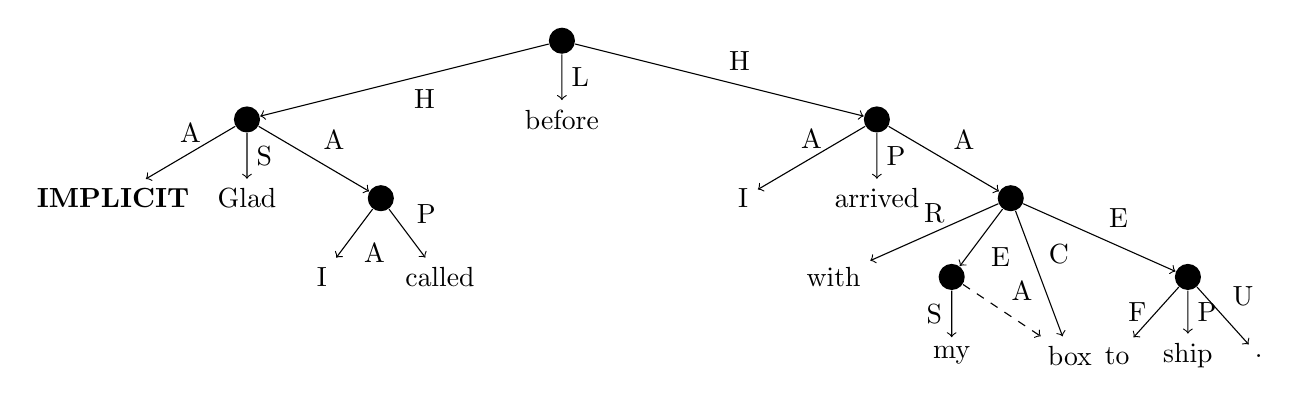
\begin{tikzpicture}[->,level distance=1cm,
  level 1/.style={sibling distance=4cm},
  level 2/.style={sibling distance=17mm},
  level 3/.style={sibling distance=15mm},
  level 4/.style={sibling distance=9mm},
  every circle node/.append style={fill=black}]
  \tikzstyle{word} = [font=\rmfamily,color=black]
  \node (1_1) [circle] {}
  {
  child {node (1_2) [circle] {}
    {
    child {node (1_16) [word] {\textbf{IMPLICIT}}  edge from parent node[above]  {A}}
    child {node (1_17) [word] {Glad}  edge from parent node[auto]  {S}}
    child {node (1_18) [circle] {}
      {
      child {node (1_19) [word] {I}  edge from parent node[auto]  {A}}
      child {node (1_20) [word] {called}  edge from parent node[auto]  {P}}
      } edge from parent node[auto]  {A}}
    } edge from parent node[auto]  {H}}
  child {node (1_3) [word] {before}  edge from parent node[auto]  {L}}
  child {node (1_4) [circle] {}
    {
    child {node (1_6) [word] {I}  edge from parent node[above]  {A}}
    child {node (1_7) [word] {arrived}  edge from parent node[auto]  {P}}
    child {node (1_8) [circle] {}
      {
      child {node (1_9) [word] {with}  edge from parent node[above]  {R}}
      child {node (1_10) [circle] {}
        {
        child {node (1_15) [word] {my}  edge from parent node[left]  {S}}
        } edge from parent node[auto]  {E}}
      child {node {}
        {
        child {node (1_11) [word] {box}  edge from parent [draw=none] {}}
        } edge from parent [draw=none] {}}
      child {node (1_12) [circle] {}
        {
        child {node (1_13) [word] {to}  edge from parent node[left]  {F}}
        child {node (1_14) [word] {ship}  edge from parent node[auto]  {P}}
        child {node (1_21) [word] {.}  edge from parent node[auto]  {U}}
        } edge from parent node[auto]  {E}}
      } edge from parent node[auto]  {A}}
    } edge from parent node[auto]  {H}}
  };
  \draw[dashed,->] (1_10) to node [auto] {A} (1_11);
  \draw[->] (1_8) to node [auto] {C} (1_11);
\end{tikzpicture}
\caption{UCCA example including an implicit node, where the subject of ``Glad'' is omitted.}\label{fig:implicit}
\end{figure}
\begin{figure}[ht]\small\centering
  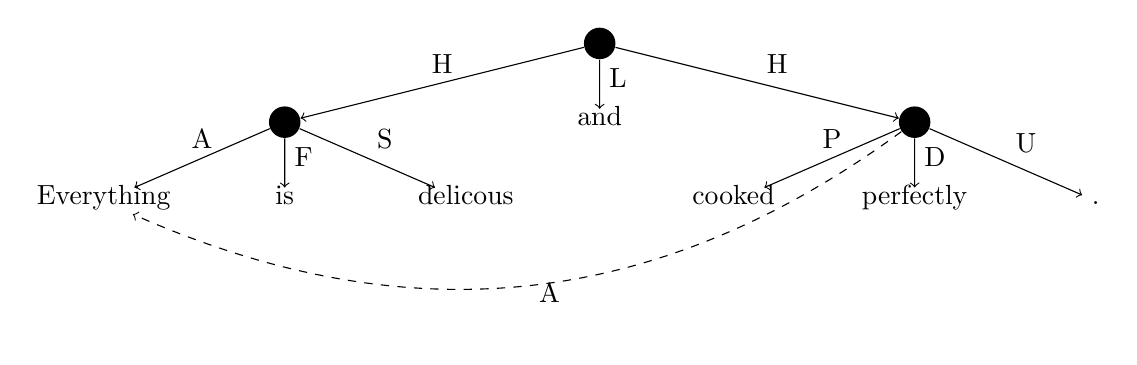
\begin{tikzpicture}[->,level distance=1cm,
  level 1/.style={sibling distance=4cm},
  level 2/.style={sibling distance=23mm},
  level 3/.style={sibling distance=15mm},
  every circle node/.append style={fill=black},
  every node/.append style={text height=.6ex,text depth=0}]
  \tikzstyle{word} = [font=\rmfamily,color=black]
  \node (1_1) [circle] {}
  {
  child {node (1_2) [circle] {}
    {
    child {node (1_8) [word] {Everything}  edge from parent node[above]  {A}}
    child {node (1_9) [word] {is}  edge from parent node[auto]  {F}}
    child {node (1_10) [word] {delicous}  edge from parent node[auto]  {S}}
    } edge from parent node[above]  {H}}
  child {node (1_3) [word] {and}  edge from parent node[auto]  {L}}
  child {node (1_4) [circle] {}
    {
    child {node (1_6) [word] {cooked}  edge from parent node[above]  {P}}
    child {node (1_7) [word] {perfectly}  edge from parent node[auto]  {D}}
    child {node (1_11) [word] {.}  edge from parent node[auto]  {U}}
    } edge from parent node[auto]  {H}}
  };
  \draw[dashed,->,bend left] (1_4) to node [auto] {A} (1_8);
\end{tikzpicture}
\caption{
    UCCA example including a remote edge (dashed),
    resulting in ``Everything'' having two parents.}\label{fig:remote}
\end{figure}
\begin{figure}[ht]\small
  \begin{subfigure}{.45\textwidth}
  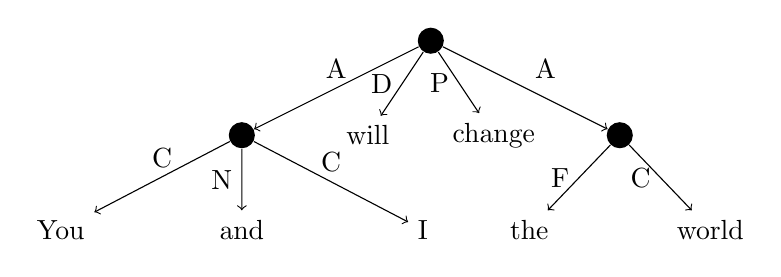
\begin{tikzpicture}[level distance=12mm, ->,
  level 1/.style={sibling distance=16mm},
  level 2/.style={sibling distance=23mm},
  level 3/.style={sibling distance=15mm},
      every node/.append style={midway}]
    \node (ROOT) [fill=black, circle] {}
      child {node [fill=black, circle] {}
      {
        child {node {You} edge from parent node[above] {C}}
        child {node {and} edge from parent node[left] {N}}
        child {node {I} edge from parent node[above] {C}}
      } edge from parent node[above] {A} }
      child {node {will} edge from parent node[left] {D}}
      child {node {change} edge from parent node[left] {P}}
      child {node [fill=black, circle] {}
      {
        child {node {the} edge from parent node[left] {F}}
        child {node {world} edge from parent node[left] {C}}
      } edge from parent node[auto] {A} }
      ;
  \end{tikzpicture}
  \caption{}\label{fig:changetheworld}
  \end{subfigure}\hfill
  \begin{subfigure}{.45\textwidth}
  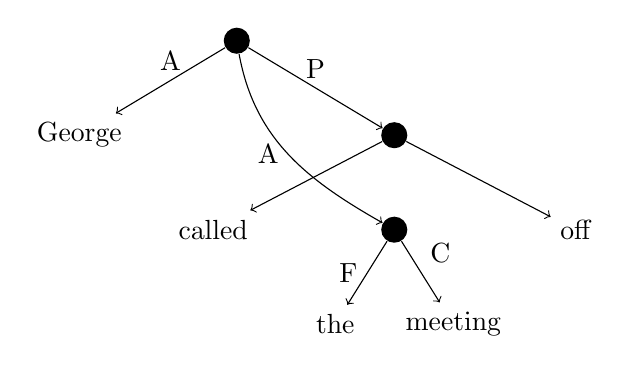
\begin{tikzpicture}[level distance=12mm, ->,
  level 1/.style={sibling distance=4cm},
  level 2/.style={sibling distance=23mm},
  level 3/.style={sibling distance=15mm},
      every node/.append style={midway}]
    \node (ROOT) [fill=black, circle] {}
      child {node {George} edge from parent node[above] {A}}
      child {node [fill=black, circle] {}
      {
      	child {node {called} edge from parent node[right] {}}
      	child {node (themeeting) [fill=black, circle] {}
        {
      	  child {node {the} edge from parent [black] node[left] {F}}
      	  child {node {meeting} edge from parent [black] node[auto] {C}}
      	} edge from parent[white]}
      	child {node {off} edge from parent node[above] {}}
      } edge from parent node[above] {P} }
      ;
    \draw[bend right,->] (ROOT) to[out=-30, in=200] node [left] {A} (themeeting);
  \end{tikzpicture}
  \caption{}\label{fig:calledoff}
  \end{subfigure}
  \caption{\label{fig:examples}
    UCCA examples.
    (\subref{fig:changetheworld}) includes a coordination construction (``You and I'').
    (\subref{fig:calledoff}) includes a discontinuous unit (``called ... off'').
  }
\end{figure}

\section{UCCA Parsing}

In order to represent the full range of semantic structures exhibited by
natural language, three properties should be supported: reentrancy,
representing arguments shared between predicates;
non-terminal nodes for multi-word units;
and discontinuity of semantic units in the text.

The first property, \textbf{reentrancy} (or \textbf{multiple parents}), is required for
representing arguments and relations (semantic units) that are shared between predicates.
For instance, in the sentence
``Everything is delicious and cooked perfectly'' (Figure~\ref{fig:remote}),
``Everything'' is an argument of both ``delicious''
and ``cooked perfectly'', yielding a DAG structure rather than a tree.

The second is \textbf{non-terminal nodes} for representing units
comprising more than one word (Figure~\ref{fig:changetheworld}).
While bi-lexical dependencies partially circumvent this requirement, by
representing complex units in terms of their headwords, they fall short
when representing units that have no clear head.
Frequent examples of such constructions include
coordination structures (e.g., ``\textit{You and I} will change the world''),
some multi-word expressions (e.g., ``The Haves and the \textit{Have Nots}''),
and prepositional phrases.
In these cases, dependency schemes often apply some annotation convention that
selects one of the sub-units
as the head, but as different head selections are needed for different purposes,
standardization problems arise \citep{Ivanova2012who}.
For example, selecting the preposition to head prepositional phrases yields better
parsing results \citep{Schwartz:12}, while the head noun can be more useful for
information extraction purposes.

Third, semantic units may be \textbf{discontinuous} in the text. For instance, in
``George \textit{called} the meeting \textit{off}'' (Figure~\ref{fig:calledoff}),
the phrasal verb ``called ... off'' forms a single semantic unit.
Discontinuities are also pervasive with other multi-word
expressions \citep{schneider2014discriminative}.

The only semantic annotation scheme that supports the combination of these criteria is UCCA
\citep{abend2013universal},
for which no parser has existed prior to my work.

My research is concerned with learning to parse UCCA graphs from text, representing its semantics.
I introduce a general graph parser,
and investigate the relationship with other representations to find beneficial commonalities and
differences highlighting the potential utility of semantic parsers for text understanding applications.
The analysis also exposes challenges semantic parsers must address,
and potential sources for improvement.

To summarize, this thesis has the following goals:
developing techniques for general graph parsing, and
specifically, devising a method for automatic prediction of UCCA
    structure given plain text;
investigating and quantifying the relationship between the content
    captured in UCCA and other semantic or syntactic representations;
and taking advantage of the similarities to other schemes,
    to improve UCCA parsing by learning common distinctions.

\chapter{Methodology}

\subsection*{Transition-Based Parsing}

Transition-based parsers \citep{Nivre03anefficient} build trees or graphs
as they scan the text incrementally.
The parse is created by applying a \textit{transition} at each step to the parser state,
defined using a buffer of tokens and nodes to be processed,
a stack of nodes currently being processed,
and a graph of constructed nodes and labeled edges.
A classifier is used at each step to select the next transition based on features
that encode the parser's current state.
During training, an oracle creates training instances for the classifier,
based on the gold-standard annotation.

The transition-based approach has produced some of the best
results in syntactic dependency parsing
\citep{kiperwasser2016simple,andor2016globally}, and has also demonstrated
strong performance in a variety of other semantic and syntactic settings
\citep{maier2015discontinuous,damonte-17}.
Transition-based methods are a natural starting point for UCCA parsing,
as the set of distinctions it represents is similar in spirit to the distinctions
conveyed by dependency schemes.


\subsection*{Neural Networks}

Neural networks are powerful machine learning models.
They have yielded state-of-the-art results in many fields,
including natural language processing \citep{goldberg2016primer}.
Inspired by the brain's computation mechanism,
artificial neural networks operate on dense input representations
by a combination of linear and non-linear transformations.

Language data is commonly manifested as sequences
(e.g., sentences are sequences of words).
Recurrent neural networks \citep{elman1990finding} allow representing
arbitrarily sized sequences in a fixed-size vector,
without ignoring the structured properties of the input.
A specific flavor called Long Short Term Memory
(LSTM) is very common as it learns relatively long-term dependencies.
A bidirectional recurrent neural network, such as a BiLSTM,
takes into account both the past and future.


\subsection*{Multitask Learning}

Multitask learning \citep{caruana1998multitask} allows exploiting the overlap between tasks
to effectively extend the training data, 
and has greatly advanced with neural networks and representation learning.
It has been used over the years for NLP tasks with varying degrees of similarity.

Neural multitask learning has mostly been effective in tackling formally similar
tasks \citep{P16-2038},
including
multilingual syntactic dependency parsing \citep{Q16-1031,guo2016exploiting},
as well as multilingual \citep{duong2017multilingual},
and cross-domain semantic parsing \citep{herzig-berant:2017:Short,W17-2607}.

Sharing parameters with a low-level task
has shown great benefit for transition-based syntactic parsing
\citep{bohnet2012transition,Zhang2016StackpropagationIR,constant-nivre:2016:P16-1,more2016joint}.
Recent work has achieved state-of-the-art results in multiple NLP tasks
by jointly learning the tasks forming the NLP standard pipeline using 
a single neural model \citep{collobert2011natural,D17-1206},
thereby avoiding cascading errors, common in pipelines.


\subsection*{Evaluation}
Comparing UCCA structures
$G_p=(V_p,E_p,\ell_p)$ and $G_g=(V_g,E_g,\ell_g)$,
over the same sequence of terminals $W = \{w_1,\ldots,w_n\}$
is done as follows.
For an edge $e=(u,v)$ in either graph, its yield $y(e) \subseteq W$ is the
set of terminals in $W$ that are descendants of $v$.
Define the set of \textit{mutual edges} between $G_p$ and $G_g$:
\[
    M(G_p,G_g) =
    \left\{(e_1,e_2) \in E_p \times E_g \;|\;
    y(e_1) = y(e_2) \wedge \ell_p(e_1)=\ell_g(e_2)\right\}
\]

Labeled precision and recall are defined by dividing $|M(G_p,G_g)|$ by $|E_p|$ and $|E_g|$, respectively,
and F-score by taking their harmonic mean.
Two variants are reported: one where we consider only primary edges,
and another for remote edges


%
% File acl2017.tex
%

\chapter{A Transition-Based Directed Acyclic Graph Parser for UCCA (Published in ACL 2017)}

\subsubsection*{Daniel Hershcovich$^{1,2}$, Omri Abend$^2$ and Ari Rappoport$^2$ \\
  $^1$The Edmond and Lily Safra Center for Brain Sciences \\
  $^2$School of Computer Science and Engineering \\
  Hebrew University of Jerusalem \\
  \texttt{\{danielh,oabend,arir\}@cs.huji.ac.il}  
}

%%%%%%%%%%%%%%%%%%%%%%%%%%%%%%%%%%%%%%%%%%%%%%%%%%%%%%%%%%%%%%%
%%%%%%%%%%%%%%%%%     Abstract     %%%%%%%%%%%%%%%%%%%%%%%%%%%%
%%%%%%%%%%%%%%%%%%%%%%%%%%%%%%%%%%%%%%%%%%%%%%%%%%%%%%%%%%%%%%%
\section*{Abstract}
  We present the first parser for UCCA, a
  cross-linguistically applicable framework for semantic
  representation, which builds on extensive
  typological work and supports rapid annotation.
  UCCA poses a challenge for existing parsing techniques,
  as it exhibits reentrancy (resulting in DAG structures),
  discontinuous structures and non-terminal nodes corresponding
  to complex semantic units. To our knowledge, the conjunction
  of these formal properties is not supported by any existing parser.
  Our transition-based parser, which uses a novel transition set
  and features based on bidirectional LSTMs,
  has value not just for UCCA parsing:
  its ability to handle more general graph structures can inform
  the development of parsers for other semantic DAG structures, 
  and in languages that frequently use discontinuous structures.


%%%%%%%%%%%%%%%%%%%%%%%%%%%%%%%%%%%%%%%%%%%%%%%%%%%%%%%%%%%%%%%
\section{Introduction}\label{sec:introductiona}

Universal Conceptual Cognitive Annotation \cite[UCCA,][]{abend2013universal}
is a cross-linguistically applicable semantic representation scheme,
building on the established Basic Linguistic Theory typological framework
\cite{Dixon:10b,Dixon:10a,Dixon:12}, and Cognitive
Linguistics literature \cite{croft2004cognitive}.
It has demonstrated applicability to multiple languages, including
English, French, German and Czech,
support for rapid annotation by non-experts
(assisted by an accessible annotation interface \cite{abend2017uccaapp}),
and stability under translation \cite{sulem2015conceptual}.
It has also proven useful for machine translation evaluation \cite{birch2016hume}.
UCCA differs from syntactic
schemes in terms of content and formal structure.
It exhibits reentrancy, discontinuous nodes and non-terminals,
which no single existing parser supports.
Lacking a parser, UCCA's applicability has been so far limited,
a gap this work addresses.

We present the first UCCA parser, \parser{}
(Transition-based UCCA Parser),
building on recent advances in discontinuous constituency
and dependency graph parsing, and further introducing novel transitions and features for UCCA.
Transition-based techniques are a natural
starting point for UCCA parsing, given the conceptual similarity of
UCCA's distinctions, centered around predicate-argument structures, to distinctions expressed
by dependency schemes, and the achievements of transition-based methods in dependency parsing
\cite{dyer2015transition,andor2016globally,kiperwasser2016simple}.
We are further motivated by the strength of transition-based methods
in related tasks, including dependency graph parsing
\cite{sagae2008shift,ribeyre-villemontedelaclergerie-seddah:2014:SemEval,tokgoz2015transition},
constituency parsing \cite{sagae2005classifier,zhang2009transition,zhu2013fast,maier2015discontinuous,maier-lichte:2016:DiscoNLP},
AMR parsing \cite{wang-xue-pradhan:2015:ACL-IJCNLP,wang2015transition,wang-EtAl:2016:SemEval,dipendra2016neural,goodman2016noise,zhou2016amr,damonte-17}
and CCG parsing \cite{zhang2011shift,ambati2015incremental,ambati-deoskar-steedman:2016:N16-1}.

We evaluate \parser{} on the English UCCA corpora, including in-domain and out-of-domain settings.
To assess the ability of existing
parsers to tackle the task, we develop a conversion procedure
from UCCA to bilexical graphs and trees.
Results show superior performance for \parser{}, demonstrating the effectiveness of
the presented approach.\footnote{All parsing and conversion code, as well as trained parser models,
are available at \url{https://github.com/danielhers/tupa}.}

The rest of the paper is structured as follows:
\secref{sec:uccaa} describes UCCA in more detail.
\secref{sec:parser} introduces \parser{}.
\secref{sec:exp_setup} discusses the data and experimental setup.
\secref{sec:resultsa} presents the experimental results.
\secref{sec:related_worka} summarizes related work, and
\secref{sec:conclusiona} concludes the paper.




%%%%%%%%%%%%%%%%%%%%%%%%%%%%%%%%%%%%%%%%%%%%%%%%%%%%%%%%%%%%%%%
\section{The UCCA Scheme}\label{sec:uccaa}

UCCA graphs are labeled, directed acyclic graphs (DAGs),
whose leaves correspond to the tokens of
the text. A node (or {\it unit}) corresponds to a terminal or
to several terminals (not necessarily contiguous) viewed as a
single entity according to semantic or cognitive considerations.
Edges bear a category, indicating the role of the sub-unit in the parent relation.
\figref{fig:examplesa} presents a few examples.

UCCA is a multi-layered representation, where each layer corresponds
to a ``module'' of semantic distinctions.
UCCA's \textit{foundational layer}, targeted in this paper, covers the predicate-argument
structure evoked by predicates of all grammatical categories
(verbal, nominal, adjectival and others), the inter-relations between them,
and other major linguistic phenomena such as coordination and multi-word expressions.
The layer's basic notion is the \textit{scene},
describing a state, action, movement or some other relation that evolves in time.
Each scene contains one main relation (marked as either a Process or a State),
as well as one or more Participants.
For example, the sentence ``After graduation, John moved to Paris'' (\figref{fig:graduationa})
contains two scenes, whose main relations are ``graduation'' and ``moved''.
``John'' is a Participant in both scenes, while ``Paris'' only in the latter.
Further categories account for inter-scene relations and the internal structure of
complex arguments and relations (e.g. coordination, multi-word expressions and modification).

One incoming edge for each non-root node is marked as \textit{primary},
and the rest (mostly used for implicit relations and arguments) as \textit{remote} edges,
a distinction made by the annotator.
The primary edges thus form a tree structure, whereas the remote edges enable reentrancy,
forming a DAG.

\begin{figure}[t]
  \begin{subfigure}{.9\columnwidth}
  \parbox{.05\columnwidth}{\caption{}\label{fig:graduationa}}
  \parbox{.8\columnwidth}{
  \scalebox{.9}{
  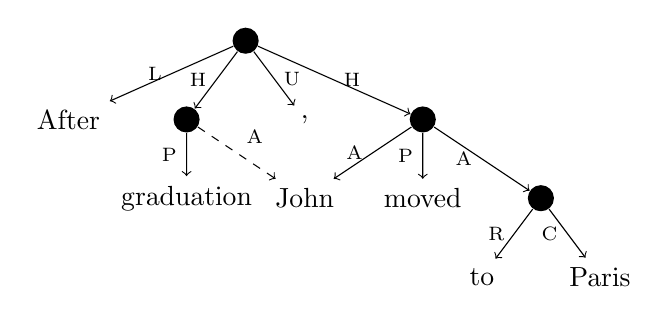
\begin{tikzpicture}[level distance=10mm, ->,
      every circle node/.append style={fill=black}]
    \node (ROOT) [circle] {}
      child {node (After) {After} edge from parent node[left] {\scriptsize L}}
      child {node (graduation) [circle] {}
      {
        child {node {graduation} edge from parent node[left] {\scriptsize P}}
      } edge from parent node[left] {\scriptsize H} }
      child {node {,} edge from parent node[right] {\scriptsize U}}
      child {node (moved) [circle] {}
      {
        child {node (John) {John} edge from parent node[left] {\scriptsize A}}
        child {node {moved} edge from parent node[left] {\scriptsize P}}
        child {node [circle] {}
        {
          child {node {to} edge from parent node[left] {\scriptsize R}}
          child {node {Paris} edge from parent node[left] {\scriptsize C}}
        } edge from parent node[left] {\scriptsize A} }
      } edge from parent node[right] {\scriptsize H} }
      ;
    \draw[dashed,->] (graduation) to node [auto] {\scriptsize A} (John);
  \end{tikzpicture}
  }}
  \end{subfigure}
  \begin{subfigure}{.9\columnwidth}
  \vspace{-2cm}
  \parbox{.05\columnwidth}{\caption{}\label{fig:gavea}}
  \parbox{.75\columnwidth}{\hspace{1cm}
  \scalebox{.9}{
  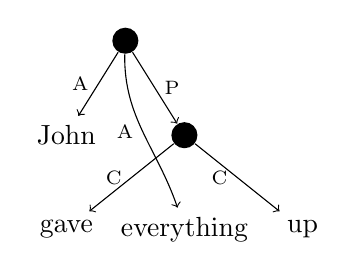
\begin{tikzpicture}[level distance=12mm, ->,
      every node/.append style={midway},
      every circle node/.append style={fill=black}]
    \node (ROOT) [circle] {}
      child {node {John} edge from parent node[left] {\scriptsize A}}
      child {node [circle] {}
      {
      	child {node {gave} edge from parent node[left] {\scriptsize C}}
      	child {node (everything) {everything} edge from parent[white]}
      	child {node {up} edge from parent node[left] {\scriptsize C}}
      } edge from parent node[right] {\scriptsize P} }
      ;
    \draw[bend right,->] (ROOT) to[out=-20, in=180] node [left] {\scriptsize A} (everything);
  \end{tikzpicture}
  }}
  \parbox{.1\columnwidth}{
  \vspace{2cm}
  \begin{adjustbox}{width=.3\columnwidth,margin=1pt,frame}
  \begin{tabular}{ll}
	  P & process \\
	  A & participant \\
	  H & linked scene \\
	  C & center \\
	  R & relator \\
	  N & connector \\
	  L & scene linker \\
	  U & punctuation \\
	  F & function unit
  \end{tabular}
  \end{adjustbox}
  }
  \end{subfigure}
  \begin{subfigure}{.9\columnwidth}
  \vspace{-1cm}
  \parbox{.05\columnwidth}{\caption{}\label{fig:homea}}
  \parbox{.65\columnwidth}{
  \scalebox{.9}{
  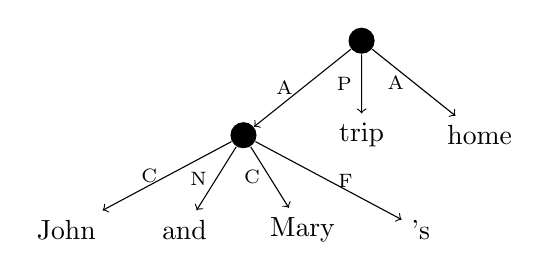
\begin{tikzpicture}[level distance=12mm, ->,
      every node/.append style={midway},
      every circle node/.append style={fill=black}]
    \node (ROOT) [circle] {}
      child {node [circle] {}
      {
        child {node {John} edge from parent node[left] {\scriptsize C}}
        child {node {and} edge from parent node[left] {\scriptsize N}}
        child {node {Mary} edge from parent node[left] {\scriptsize C}}
        child {node {'s} edge from parent node[right] {\scriptsize F}}
      } edge from parent node[left] {\scriptsize A} }
      child {node {trip} edge from parent node[left] {\scriptsize P}}
      child {node {home} edge from parent node[left] {\scriptsize A}}
      ;
  \end{tikzpicture}
  }}
  \end{subfigure}
  \caption{\label{fig:examplesa}
    UCCA structures demonstrating three structural properties exhibited by
    the scheme.
    (\subref{fig:graduationa}) includes a remote edge (dashed),
    resulting in ``John'' having two parents.
    (\subref{fig:gavea}) includes a discontinuous unit (``gave ... up'').
    (\subref{fig:homea}) includes a coordination construction (``John and Mary'').
    Pre-terminal nodes are omitted for brevity.
    Right: legend of edge labels.
  }
\end{figure}

While parsing technology in general, and transition-based parsing in particular,
is well-established for syntactic parsing, UCCA
has several distinct properties
that distinguish it from syntactic representations,
mostly UCCA's tendency to abstract away from syntactic detail that do not
affect argument structure.
%.\footnote{As essentially any change in form results
%in some change in meaning, it would be more precise to say that
%UCCA's foundational layer abstracts away from syntactic variation
%not affecting argument structure and other aspects of meaning it covers.}
For instance, consider the following examples where the concept of a scene
has a different rationale from the syntactic concept of a clause.
First, non-verbal predicates in UCCA are represented like verbal ones,
such as when they appear in copula clauses or noun phrases. Indeed,
in \figref{fig:graduationa}, ``graduation'' and ``moved'' are considered separate events,
despite appearing in the same clause. 
Second, in the same example, ``John'' is marked as a (remote) Participant
in the graduation scene, despite not being overtly marked.
Third, consider the possessive construction in \figref{fig:homea}.
While in UCCA ``trip'' evokes a scene in which ``John and Mary'' is
a Participant, a syntactic scheme would analyze this phrase similarly to ``John and Mary's shoes''.

These examples demonstrate that a UCCA parser, and more generally semantic parsers,
face an additional level of ambiguity compared to their syntactic counterparts
(e.g., ``after graduation'' is formally very similar to ``after 2pm'',
which does not evoke a scene).
\secref{sec:related_worka} discusses UCCA in the context of other semantic schemes,
such as AMR \cite{banarescu2013abstract}.

%These properties distinguish UCCA from syntactic schemes that already have
%established parsing techonology, and will likely require different techniques.

Alongside recent progress in dependency parsing into projective trees,
there is increasing interest in parsing into 
representations with more general structural properties  (see \secref{sec:related_worka}).
One such property is \textit{reentrancy},
namely the sharing of semantic units between predicates.
For instance, in \figref{fig:graduationa},
``John'' is an argument of both ``graduation''
and ``moved'', yielding a DAG rather than a tree.
A second property is \textit{discontinuity},
as in \figref{fig:gavea}, where ``gave up'' forms a discontinuous semantic unit.
Discontinuities are pervasive, e.g.,  with multi-word
expressions \cite{schneider2014discriminative}.
Finally, unlike most dependency schemes, UCCA uses \textit{non-terminal nodes}
to represent units comprising more than one word.
The use of non-terminal nodes is motivated by constructions with no clear head, including
coordination structures (e.g., ``John and Mary'' in \figref{fig:homea}),
some multi-word expressions (e.g., ``The Haves and the \textit{Have Nots}''),
and prepositional phrases (either the preposition or the head noun can serve as the constituent's head).
To our knowledge, no existing parser supports all structural properties required for UCCA
parsing.



%%%%%%%%%%%%%%%%%%%%%%%%%%%%%%%%%%%%%%%%%%%%%%%%%%%%%%%%%%%%%%%
\section{Transition-based UCCA Parsing}\label{sec:parser}

We now turn to presenting \parser{}.
Building on previous work on parsing reentrancies, discontinuities and non-terminal nodes,
we define an extended set of transitions and features that supports the conjunction of
these properties.

Transition-based parsers \cite{Nivre03anefficient} scan the text from start to end,
and create the parse incrementally by applying a \textit{transition}
at each step to the parser's state,
defined using three data structures: a buffer $B$ of tokens and nodes to be processed,
a stack $S$ of nodes currently being processed,
and a graph $G=(V,E,\ell)$ of constructed nodes and edges,
where $V$ is the set of \emph{nodes}, $E$ is the set of \emph{edges},
and $\ell : E \to L$ is the \emph{label} function, $L$ being the set of possible labels.
Some states are marked as \textit{terminal}, meaning that $G$ is the final output.
A classifier is used at each step to select the next transition based on features
encoding the parser's current state.
During training, an oracle creates training instances for the classifier,
based on gold-standard annotations.


\begin{figure*}
	\begin{adjustbox}{width=\textwidth,margin=3pt,frame}
	\begin{tabular}{llll|l|llllc|c}
		\multicolumn{4}{c|}{\textbf{\small Before Transition}} & \textbf{\small Transition} & \multicolumn{5}{c|}{\textbf{\small After Transition}} & \textbf{\small Condition} \\
		\textbf{\footnotesize Stack} & \textbf{\footnotesize Buffer} & \textbf{\footnotesize Nodes} & \textbf{\footnotesize Edges} & & \textbf{\footnotesize Stack} & \textbf{\footnotesize Buffer} & \textbf{\footnotesize Nodes} & \textbf{\footnotesize Edges} & \textbf{\footnotesize Terminal?} & \\
		$S$ & $x \;|\; B$ & $V$ & $E$ & \textsc{Shift} & $S \;|\; x$ & $B$ & $V$ & $E$ & $-$ & \\
		$S \;|\; x$ & $B$ & $V$ & $E$ & \textsc{Reduce} & $S$ & $B$ & $V$ & $E$ & $-$ & \\
		$S \;|\; x$ & $B$ & $V$ & $E$ & \textsc{Node$_X$} & $S \;|\; x$ & $y \;|\; B$ & $V \cup \{ y \}$ & $E \cup \{ (y,x)_X \}$ & $-$ &
		$x \neq \mathrm{root}$ \\
		$S \;|\; y,x$ & $B$ & $V$ & $E$ & \textsc{Left-Edge$_X$} & $S \;|\; y,x$ & $B$ & $V$ & $E \cup \{ (x,y)_X \}$ & $-$ &
		\multirow{4}{50pt}{\vspace{-5mm}\[\left\{\begin{array}{l}
		x \not\in w_{1:n},\\
		y \neq \mathrm{root},\\
		y \not\leadsto_G x
		\end{array}\right.\]} \\
		$S \;|\; x,y$ & $B$ & $V$ & $E$ & \textsc{Right-Edge$_X$} & $S \;|\; x,y$ & $B$ & $V$ & $E \cup \{ (x,y)_X \}$ & $-$ & \\
		$S \;|\; y,x$ & $B$ & $V$ & $E$ & \textsc{Left-Remote$_X$} & $S \;|\; y,x$ & $B$ & $V$ & $E \cup \{ (x,y)_X^* \}$ & $-$ & \\
		$S \;|\; x,y$ & $B$ & $V$ & $E$ & \textsc{Right-Remote$_X$} & $S \;|\; x,y$ & $B$ & $V$ & $E \cup \{ (x,y)_X^* \}$ & $-$ & \\
		$S \;|\; x,y$ & $B$ & $V$ & $E$ & \textsc{Swap} & $S \;|\; y$ & $x \;|\; B$ & $V$ & $E$ & $-$ &
		$\mathrm{i}(x) < \mathrm{i}(y)$ \\
		$[\mathrm{root}]$ & $\emptyset$ & $V$ & $E$ & \textsc{Finish} & $\emptyset$ & $\emptyset$ & $V$ & $E$ & $+$ & \\
	\end{tabular}
	\end{adjustbox}
	\caption{\label{fig:transitions}
	  The transition set of \parser{}. %Following standard practice,
	  We write the stack with its top to the right and the buffer with its head to the left.
	  $(\cdot,\cdot)_X$ denotes a primary $X$-labeled edge, and $(\cdot,\cdot)_X^*$ a remote $X$-labeled edge.
	  $\mathrm{i}(x)$ is a running index for the created nodes.
	  In addition to the specified conditions,
	  the prospective child in an \textsc{Edge} transition must not already have a primary parent.
	}
\end{figure*}

\paragraph{Transition Set.}
Given a sequence of tokens $w_1, \ldots, w_n$, we predict a UCCA graph $G$ over the sequence.
Parsing starts with a single node on the stack (an artificial root node), and the input tokens
in the buffer. \figref{fig:transitions} shows the transition set.

In addition to the standard \textsc{Shift} and \textsc{Reduce} operations, 
we follow previous work in transition-based constituency parsing \cite{sagae2005classifier},
adding the \textsc{Node} transition for creating new non-terminal nodes.
For every $X\in L$,
\textsc{Node$_X$} creates a new node on the buffer as a parent of the first element on the stack, with an $X$-labeled edge.
\textsc{Left-Edge$_X$} and \textsc{Right-Edge$_X$} create a new primary $X$-labeled edge between the first two elements on the stack, where the parent is the left or the right node, respectively.
As a UCCA node may only have one incoming primary edge,
\textsc{Edge} transitions are disallowed if the child node already
has an incoming primary edge.
\textsc{Left-Remote$_X$} and \textsc{Right-Remote$_X$} do not have this restriction,
and the created edge is additionally marked as \textit{remote}.
We distinguish between these two pairs of transitions to allow the parser to create remote edges
without the possibility of producing invalid graphs.
To support the prediction of multiple parents, node and edge transitions
leave the stack unchanged, as in other work on
transition-based dependency graph parsing
\cite{sagae2008shift,ribeyre-villemontedelaclergerie-seddah:2014:SemEval,tokgoz2015transition}.
\textsc{Reduce} pops the stack, to allow removing a node
once all its edges have been created.
To handle discontinuous nodes, \textsc{Swap} pops the second
node on the stack and adds it to the top of the buffer, as with the similarly
named transition in previous work \cite{nivre2009non,maier2015discontinuous}.
Finally, \textsc{Finish} pops the root node and marks the state as terminal.

\paragraph{Classifier.}
The choice of classifier and feature representation has been shown to play an important role in
transition-based parsing \cite{chen2014fast,andor2016globally,kiperwasser2016simple}.
To investigate the impact of the type of transition classifier in UCCA parsing,
we experiment with three different models.
\begin{enumerate}
\item
Starting with a simple and common choice \cite[e.g.,][]{maier-lichte:2016:DiscoNLP},
\textbf{\parser{Sparse}} uses a linear classifier with sparse features, trained with
the averaged structured perceptron algorithm
\cite{Coll:04} and \textsc{MinUpdate} \cite{goldberg2011learning}:
each feature requires a minimum number of updates in training
to be included in the model.\footnote{We also experimented with a linear model using
dense embedding features, trained with the averaged structured perceptron algorithm.
It performed worse than the sparse perceptron model and was hence discarded.}
\item
Changing the model to a feedforward neural network with dense embedding features,
\textbf{\parser{MLP}}
(``multi-layer perceptron''), uses an architecture similar to that of \citet{chen2014fast},
but with two rectified linear layers instead of one layer with cube activation.
The embeddings and classifier are trained jointly.
\item
Finally, \textbf{\parser{BiLSTM}} uses a bidirectional LSTM for feature representation,
on top of the dense embedding features,
an architecture similar to \citet{kiperwasser2016simple}.
The BiLSTM runs on the input tokens in forward and backward directions,
yielding a vector representation that is then concatenated with dense features representing the
parser state (e.g., existing edge labels and previous parser actions; see below).
This representation is then fed into a feedforward network similar to \parser{MLP}.
The feedforward layers, BiLSTM and embeddings are all trained jointly.
\end{enumerate}

For all classifiers, inference is performed greedily, i.e., without beam search.
Hyperparameters are tuned on the development set (see \secref{sec:exp_setup}).

\begin{figure}[t]
\centering
	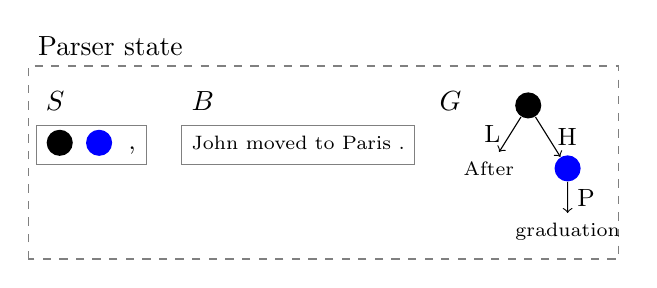
\begin{tikzpicture}[level distance=8mm, sibling distance=1cm]
	\node[anchor=west] at (0,1.5) {Parser state};
	\draw[color=gray,dashed] (0,-1.2) rectangle (7.5,1.25);
	\draw[color=gray] (.1,0) rectangle (1.5,.5);
	\node[anchor=west] at (.1,.8) {$S$};
	\node[fill=black, circle] at (.4,.275) {};
	\node[fill=blue, circle] at (.9,.275) {};
	\node[anchor=west] at (1.15,.175) {\small ,};
	\draw[color=gray] (1.95,0) rectangle (4.9,.5);
	\node[anchor=west] at (1.95,.8) {$B$};
	\node[anchor=west] at (1.95,.275) {\scriptsize John moved to Paris .};
	\node[anchor=west] at (5.1,.8) {$G$};
	\node[fill=black, circle] at (6.35,.75) {}
	  child {node  {\scriptsize After} edge from parent [->] node[left] {\small L}}
	  child {node [fill=blue, circle] {}
	  {
	    child {node {\scriptsize graduation} edge from parent [->] node[right] {\small P}}
	  } edge from parent [->] node[right] {\small H} };
	\end{tikzpicture}
	
	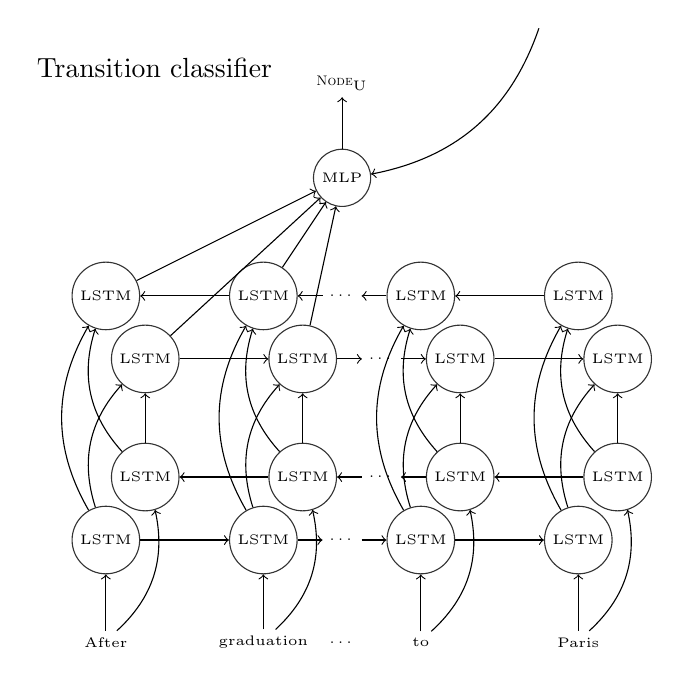
\begin{tikzpicture}[->]
	\node[anchor=west] at (0,6) {Transition classifier};
	\tiny
	\tikzstyle{main}=[circle, minimum size=7mm, draw=black!80, node distance=12mm]
	\foreach \i/\word in {1/{After},3/{graduation},5/{to},7/{Paris}} {
	    \node (x\i) at (\i,-1.3) {\word};
	    \node[main, fill=white!100] (h\i) at (\i,0) {LSTM};
        \path (x\i) edge (h\i);
	    \node[main, fill=white!100] (i\i) at (\i.5,.8) {LSTM};
        \path (x\i) edge [bend right] (i\i);
	    \node[main, fill=white!100] (l\i) at (\i.5,2.3) {LSTM};
        \path (h\i) edge [bend left] (l\i);
        \path (i\i) edge (l\i);
	    \node[main, fill=white!100] (k\i) at (\i,3.1) {LSTM};
        \path (i\i) edge [bend left] (k\i);
        \path (h\i) edge [bend left] (k\i);
	}
    \node (l4) at (4.5,2.3) {\ldots};
    \node (k4) at (4,3.1) {\ldots};
    \node (i4) at (4.5,.8) {\ldots};
    \node (h4) at (4,0) {\ldots};
    \node (x4) at (4,-1.3) {\ldots};
	\foreach \current/\next in {1/3,3/4,4/5,5/7} {
        \path (i\next) edge (i\current);
        \path (h\current) edge (h\next);
        \path (k\next) edge (k\current);
        \path (l\current) edge (l\next);
	}
    \node[main, fill=white!100] (mlp) at (4,4.6) {MLP};
	\foreach \i in {1,3} {
        \path (l\i) edge (mlp);
        \path (k\i) edge (mlp);
    }
    \coordinate (state) at (6.5,6.5);
    \path (state) edge [bend left] (mlp);
    \node (transition) at (4,5.8) {\textsc{Node}\textsubscript{U}};
    \path (mlp) edge (transition);
	\end{tikzpicture}
	\caption{Illustration of the \parser{} model.
		Top: parser state (stack, buffer and intermediate graph).
		Bottom: \parser{BiLTSM} architecture.
		Vector representation for the input tokens is computed
		by two layers of bidirectional LSTMs.
		The vectors for specific tokens are concatenated with
		embedding and numeric features from the parser state
		(for existing edge labels, number of children, etc.),
		and fed into the MLP for selecting the next transition.}
	\label{fig:model}
\end{figure}

\paragraph{Features.}
\parser{Sparse} uses binary indicator features representing
the words, POS tags, syntactic dependency labels and
existing edge labels related to the top four stack elements and the 
next three buffer elements, in addition to their children and grandchildren in the graph.
We also use bi- and trigram features based on these values \cite{zhang2009transition,zhu2013fast},
features related to discontinuous nodes
\cite[including separating punctuation and gap type]{maier2015discontinuous},
features representing existing edges and the number of parents and children,
as well as the past actions taken by the parser.
In addition, we use use a novel, UCCA-specific feature:
number of remote children.\footnote{See
Appendix~\ref{appendix:features} for a full list of used feature templates.}

For \parser{MLP} and \parser{BiLSTM},
we replace all indicator features by a
concatenation of the vector embeddings of all represented elements:
words, POS tags, syntactic dependency labels, edge labels, punctuation, gap type and parser actions.
These embeddings are initialized randomly.
We additionally use external word embeddings initialized with
pre-trained word2vec vectors \cite{mikolov2013efficient},\footnote{\url{
https://goo.gl/6ovEhC}} updated during training.
In addition to dropout between NN layers, we apply word dropout 
\cite{kiperwasser2016simple}: with a certain probability, the embedding for a
word is replaced with a zero vector. We do not apply word dropout to the external
word embeddings.

Finally, for all classifiers we add a novel real-valued feature to the input vector,
\textbf{ratio}, corresponding to the ratio between the number of terminals to number of nodes
in the graph $G$.
This feature serves as a regularizer for the creation of new nodes,
and should be beneficial for other transition-based constituency parsers too.

\paragraph{Training.}
For training the transition classifiers, we use a dynamic oracle \cite{goldberg2012dynamic},
i.e., an oracle that outputs a set of optimal transitions: when
applied to the current parser state, the gold
standard graph is reachable from the resulting state.
For example, the oracle would predict a \textsc{Node} transition if the stack 
has on its top a parent in the gold graph that has not been created,
but would predict a \textsc{Right-Edge} transition if the second stack
element is a parent of the
first element according to the gold graph and the edge between them has not been created.
The transition predicted by the classifier is deemed correct
and is applied to the parser state to reach the subsequent state,
if the transition is included in the set of optimal transitions.
Otherwise, a random optimal transition is applied,
and for the perceptron-based parser, the classifier's weights are updated according
to the perceptron update rule.

POS tags and syntactic dependency labels are extracted using spaCy
\cite{honnibal-johnson:2015:EMNLP}.\footnote{\url{https://spacy.io}}
We use the categorical cross-entropy objective function and optimize the
NN classifiers with the Adam optimizer \cite{kingma2014adam}.



%%%%%%%%%%%%%%%%%%%%%%%%%%%%%%%%%%%%%%%%%%%%%%%%%%%%%%%%%%%%%%%
\section{Experimental Setup}\label{sec:exp_setup}

\paragraph{Data.}
We conduct our experiments on the UCCA Wikipedia corpus (henceforth, \textit{Wiki}),
and use the English part of the UCCA \textit{Twenty Thousand Leagues Under the Sea}
English-French parallel corpus (henceforth, \textit{20K Leagues}) as
out-of-domain data.\footnote{\mbox{\url{http://cs.huji.ac.il/~oabend/ucca.html}}}
\tabref{table:data} presents some statistics for the two corpora.
We use passages of indices up to 676
of the \textit{Wiki} corpus as our training set, passages 688--808 as development set,
and passages 942--1028 as in-domain test set.
While UCCA edges can cross sentence boundaries, we adhere to the common
practice in semantic parsing and train our parsers on individual sentences,
discarding inter-relations between them (0.18\% of the edges).
We also discard linkage nodes and edges (as they often express inter-sentence
relations and are thus mostly redundant when applied at the sentence level)
as well as implicit nodes.\footnote{Appendix~\ref{appendix:extended_ucca}
further discusses linkage and implicit units.}
In the out-of-domain experiments, we apply the same parsers
(trained on the \textit{Wiki} training set) to the \textit{20K Leagues} corpus
without parameter re-tuning.


\begin{table}\centering
	\scalebox{.9}{
	\begin{tabular}{l|ccc|c}
		& \multicolumn{3}{c|}{Wiki} & 20K \\
		& \small Train & \small Dev & \small Test & Leagues \\
		\hline
		\# passages & 300 & 34 & 33 & 154 \\
		\# sentences & 4268 & 454 & 503 & 506 \\
		\hline
		\# nodes & 298,993 & 33,704 & 35,718 & 29,315 \\
		\% terminal & 42.96 & 43.54 & 42.87 & 42.09 \\
		\% non-term. & 58.33 & 57.60 & 58.35 & 60.01 \\
		\% discont. & 0.54 & 0.53 & 0.44 & 0.81 \\
		\% reentrant & 2.38 & 1.88 & 2.15 & 2.03 \\
		\hline
		\# edges & 287,914 & 32,460 & 34,336 & 27,749 \\
		\% primary & 98.25 & 98.75 & 98.74 & 97.73 \\
		\% remote & 1.75 & 1.25 & 1.26 & 2.27 \\
		\hline
		\multicolumn{3}{l}{\footnotesize Average per non-terminal node} \\
		\# children & 1.67 & 1.68 & 1.66 & 1.61 
	\end{tabular}
	}
	\caption{Statistics of the \textit{Wiki} and \textit{20K Leagues} UCCA corpora.
		All counts exclude the root node, implicit nodes, and linkage nodes and edges.
	}
	\label{table:data}
\end{table}

\paragraph{Implementation.}
We use the DyNet package \cite{neubig2017dynet} for implementing the NN classifiers.
Unless otherwise noted, we use the default values provided by the package.
See Appendix~\ref{appendix:hyperparameters} for the hyperparameter values we found by tuning
on the development set.

\paragraph{Evaluation.}
We define a simple measure for comparing UCCA structures
$G_p=(V_p,E_p,\ell_p)$ and $G_g=(V_g,E_g,\ell_g)$,
the predicted and gold-standard graphs, respectively, over the same
sequence of terminals $W = \{w_1,\ldots,w_n\}$.
For an edge $e=(u,v)$ in either graph,
$u$ being the parent and $v$ the child, its yield $y(e) \subseteq W$ is the
set of terminals in $W$ that are descendants of $v$.
Define the set of \textit{mutual edges} between $G_p$ and $G_g$:

\vspace{-.6cm}

{\small
\begin{multline*}
    M(G_p,G_g) = 
    \left\{(e_1,e_2) \in E_p \times E_g \;|\;
    y(e_1) = y(e_2) \wedge \ell_p(e_1)=\ell_g(e_2)\right\}
\end{multline*}
}

\vspace{-.6cm}

Labeled precision and recall are defined by dividing $|M(G_p,G_g)|$ by $|E_p|$ and $|E_g|$, respectively,
and F-score by taking their harmonic mean.
We report two variants of this measure: one where we consider only primary edges,
and another for remote edges (see \secref{sec:uccaa}).
Performance on remote edges is of pivotal importance in this investigation,
which focuses on extending the class of graphs supported by statistical parsers.

We note that the measure collapses to the standard
PARSEVAL constituency evaluation measure if $G_p$ and $G_g$ are trees.
Punctuation is excluded from the evaluation, but not from the datasets.

\begin{figure}
	\centering
	\scalebox{.9}{
	\begin{dependency}[theme = simple]
	\begin{deptext}[column sep=.7em,ampersand replacement=\^]
	After \^ graduation \^ , \^ John \^ moved \^ to \^ Paris \\
	\end{deptext}
		\depedge{2}{1}{L}
		\depedge[edge start x offset=7pt]{2}{3}{U}
		\depedge[edge start x offset=3pt,dashed]{2}{4}{A}
		\depedge{5}{4}{A}
		\depedge{2}{5}{H}
		\depedge{7}{6}{R}
		\depedge{5}{7}{A}
	\end{dependency}
	}
	\scalebox{.9}{
	\begin{dependency}[theme = simple]
	\begin{deptext}[column sep=.7em,ampersand replacement=\^]
	John \^ gave \^ everything \^ up \\
	\end{deptext}
		\depedge{2}{1}{A}
		\depedge{2}{3}{A}
		\depedge{2}{4}{C}
	\end{dependency}
	}
	\scalebox{.9}{
	\begin{dependency}[theme = simple]
	\begin{deptext}[column sep=.7em,ampersand replacement=\^]
	John \^ and \^ Mary \^ went \^ home \\
	\end{deptext}
		\depedge{4}{1}{A}
		\depedge[edge start x offset=3pt]{1}{2}{N}
		\depedge{1}{3}{C}
		\depedge{4}{5}{A}
	\end{dependency}
	}
	\caption{Bilexical graph approximation (dependency graph) for the sentences in \figref{fig:examplesa}.}
	\label{fig:bilexical_example}
\end{figure}

\begin{table*}\small
	\begin{tabular}{l|ccc|ccc||ccc|ccc}
		& \multicolumn{6}{c||}{Wiki (in-domain)} & \multicolumn{6}{c}{20K Leagues (out-of-domain)} \\
		& \multicolumn{3}{c|}{Primary} & \multicolumn{3}{c||}{Remote}
		& \multicolumn{3}{c|}{Primary} & \multicolumn{3}{c}{Remote} \\
		& \textbf{LP} & \textbf{LR} & \textbf{LF} & \textbf{LP} & \textbf{LR} & \textbf{LF}
		& \textbf{LP} & \textbf{LR} & \textbf{LF} & \textbf{LP} & \textbf{LR} & \textbf{LF} \\
		\hline
		\parser{Sparse}
		& 64.5 & 63.7 & 64.1 & 19.8 & 13.4 & 16
		& 59.6 & 59.9 & 59.8 & 22.2 & 7.7 & 11.5 \\
		%\parser{Dense} 
		%& 59.1 & 58.9 & 59 & 17.4 & 12.4 & 14.5
		%& 57.0 & 57.9 & 57.4 & 10.8 & 4.2 & 6.0 \\
		\parser{MLP}
		& 65.2 & 64.6 & 64.9 & 23.7 & 13.2 & 16.9
		& 62.3 & 62.6 & 62.5 & 20.9 & 6.3 & 9.7 \\
		\parser{BiLSTM}
		& 74.4 & 72.7 & \textbf{73.5} & 47.4 & 51.6 & \textbf{49.4}
		& 68.7 & 68.5 & \textbf{68.6} & 38.6 & 18.8 & \textbf{25.3} \\
		\hline
		\multicolumn{8}{l}{\rule{0pt}{2ex} \footnotesize
		Bilexical Approximation (Dependency DAG Parsers)} \\
		\small Upper Bound
		%& \small 94.5 & \small 87.7 & \small 91 & \small 77.3 & \small 46.8 & \small 58.3
		%& \small 94.8 & \small 88 & \small 91.3 & \small 66.3 & \small 32.3 & \small 43.4 \\
		& & & \small 91 & & & \small 58.3
		& & & \small 91.3 & & & \small 43.4 \\
		DAGParser
		& 61.8 & 55.8 & 58.6 & 9.5 & 0.5 & 1
		& 56.4 & 50.6 & 53.4 & -- & 0 & 0 \\
		TurboParser
		& 57.7 & 46 & 51.2 & 77.8 & 1.8 & 3.7
		& 50.3 & 37.7 & 43.1 & 100 & 0.4 & 0.8 \\
		\hline
		\multicolumn{8}{l}{\rule{0pt}{2ex} \footnotesize
		Tree Approximation (Constituency Tree Parser)} \\
		\small Upper Bound
		%& \small 100 & \small 100 & \small 100 & & &
		%& \small 100 & \small 100 & \small 100 \\
		& & & \small 100 & & & \small --
		& & & \small 100 & & & \small -- \\
		\textsc{uparse}
		& 60.9 & 61.2 & 61.1 & -- & -- & --
		& 52.7 & 52.8 & 52.8 & -- & -- & -- \\
		\hline
		\multicolumn{8}{l}{\rule{0pt}{2ex} \footnotesize
		Bilexical Tree Approximation (Dependency Tree Parsers)} \\
		\small Upper Bound
		%& \small 94.5 & \small 87.7 & \small 91 & & &
		%& \small 94.8 & \small 88 & \small 91.3 \\
		& & & \small 91 & & & \small --
		& & & \small 91.3 & & & \small -- \\
		MaltParser
		& 62.8 & 57.7 & 60.2 & -- & -- & --
		& 57.8 & 53 & 55.3 & -- & -- & -- \\
		LSTM Parser
		& 73.2 & 66.9 & 69.9 & -- & -- & --
		& 66.1 & 61.1 & 63.5 & -- & -- & --
	\end{tabular}
	\caption{
	  Experimental results, in percents, on the \textit{Wiki} test set (left)
	  and the \textit{20K Leagues} set (right).
	  Columns correspond to labeled precision, recall and F-score,
	  for both primary and remote edges.
	  F-score upper bounds are reported for the conversions.
	  For the tree approximation experiments, only primary edges scores are reported,
	  as they are unable to predict remote edges.
	  \parser{BiLSTM} obtains the highest F-scores in all metrics, surpassing the
	  bilexical parsers, tree parsers and other classifiers.
	}
	\label{table:results}
\end{table*}

\paragraph{Comparison to bilexical graph parsers.}
As no direct comparison with existing parsers is possible,
we compare \parser{} to bilexical dependency graph parsers,
which support reentrancy and discontinuity but not non-terminal nodes.

To facilitate the comparison, we convert our training set into bilexical graphs
(see examples in \figref{fig:bilexical_example}),
train each of the parsers, and evaluate them by applying them to the test set
and then reconstructing UCCA graphs, which are compared with the gold standard.
The conversion to bilexical graphs is done by heuristically selecting a head terminal for each
non-terminal node, and attaching all terminal descendents to the head terminal.
In the inverse conversion, we traverse the bilexical graph in topological order,
creating non-terminal parents for all terminals, and attaching them to the previously-created
non-terminals corresponding to the bilexical
heads.\footnote{See Appendix~\ref{appendix:conversion} for a detailed description of
the conversion procedures.}

In \secref{sec:resultsa} we report the upper bounds on the achievable scores due to the
error resulting from the removal of non-terminal nodes.

\begin{figure}
	\centering
	\scalebox{.9}{
	  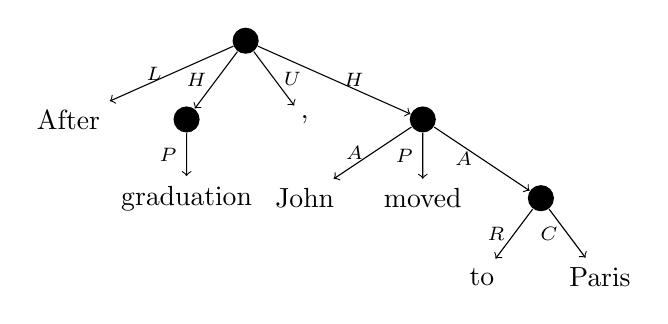
\begin{tikzpicture}[level distance=10mm, ->]
	    \node (ROOT) [fill=black, circle] {}
	      child {node (After) {After} edge from parent node[left] {\scriptsize $L$}}
	      child {node (graduation) [fill=black, circle] {}
	      {
	        child {node {graduation} edge from parent node[left] {\scriptsize $P$}}
	      } edge from parent node[left] {\scriptsize $H$} }
	      child {node {,} edge from parent node[right] {\scriptsize $U$}}
	      child {node (moved) [fill=black, circle] {}
	      {
	        child {node (John) {John} edge from parent node[left] {\scriptsize $A$}}
	        child {node {moved} edge from parent node[left] {\scriptsize $P$}}
	        child {node [fill=black, circle] {}
	        {
	          child {node {to} edge from parent node[left] {\scriptsize $R$}}
	          child {node {Paris} edge from parent node[left] {\scriptsize $C$}}
	        } edge from parent node[left] {\scriptsize $A$} }
	      } edge from parent node[right] {\scriptsize $H$} }
	      ;
	  \end{tikzpicture}
	}
	\scalebox{.9}{
	\begin{dependency}[theme = simple]
	\begin{deptext}[column sep=.7em,ampersand replacement=\^]
	After \^ graduation \^ , \^ John \^ moved \^ to \^ Paris \\
	\end{deptext}
		\depedge{2}{1}{L}
		\depedge{2}{3}{U}
		\depedge{5}{4}{A}
		\depedge{2}{5}{H}
		\depedge{7}{6}{R}
		\depedge{5}{7}{A}
	\end{dependency}
  }
  \caption{Tree approximation (constituency) for the sentence in \figref{fig:graduationa} (top),
  and bilexical tree approximation (dependency) for the same sentence (bottom).
  These are identical to the original graphs,
  apart from the removal of remote edges.}
  \label{fig:tree_example}
\end{figure}

\paragraph{Comparison to tree parsers.}
For completeness,
and as parsing technology is considerably more mature for tree (rather than graph) parsing,
we also perform a \textit{tree approximation} experiment, converting UCCA to (bilexical) trees
and evaluating constituency and dependency tree parsers on them
(see examples in \figref{fig:tree_example}).
Our approach is similar
to the tree approximation approach used for dependency graph parsing
\cite{agic2015semantic,fernandez2015parsing},
where dependency graphs were converted into dependency trees
and then parsed by dependency tree parsers.
In our setting, the conversion to trees consists simply of removing remote edges from the 
graph, and then to bilexical trees by applying the same procedure as for bilexical graphs.

\paragraph{Baseline parsers.}
We evaluate two bilexical graph semantic dependency parsers:
DAGParser \cite{ribeyre-villemontedelaclergerie-seddah:2014:SemEval}, the leading 
transition-based parser in SemEval 2014 \cite{oepen2014semeval} and
TurboParser \cite{almeida-martins:2015:SemEval},
a graph-based parser from SemEval 2015 
\cite{oepen2015semeval};
\textsc{uparse} \cite{maier-lichte:2016:DiscoNLP},
a transition-based constituency parser supporting discontinuous constituents;
and two bilexical tree parsers:
MaltParser \cite{nivre2007maltparser},
and the stack LSTM-based parser of
\citet[henceforce ``LSTM Parser'']{dyer2015transition}.
Default settings are used in all cases.\footnote{For
MaltParser we use the \textsc{ArcEager} transition set and SVM classifier.
Other configurations yielded lower scores.}
DAGParser and \textsc{uparse} use beam search by default, with a beam size of 5 and 4
respectively. The other parsers are greedy.



%%%%%%%%%%%%%%%%%%%%%%%%%%%%%%%%%%%%%%%%%%%%%%%%%%%%%%%%%%%%%%%
\section{Results}\label{sec:resultsa}

\tabref{table:results} presents our main experimental results, as well as
upper bounds for the baseline parsers,
reflecting the error resulting from the conversion.\footnote{The low
upper bound for remote edges is partly due to the removal of implicit nodes (not supported
in bilexical representations), where the whole sub-graph headed by such nodes,
often containing remote edges, must be discarded.}

DAGParser and \textsc{uparse} are most directly comparable to
\parser{Sparse}, as they also use a perceptron classifier with sparse features.
\parser{Sparse} considerably outperforms both, where
DAGParser does not predict any remote edges in the out-of-domain setting.
TurboParser fares worse in this comparison, despite somewhat better results on
remote edges.
The LSTM parser of \citet{dyer2015transition} obtains the highest primary F-score
among the baseline parsers, with a considerable margin.
%It obtains 9.7\% F-score higher than MaltParser,
%despite being limited by the same approximation error upper bound,
%and using a similar transition set.
%The performance difference between them should therefore be attributed to the classification model.

Using a feedforward NN and embedding features,
\parser{MLP} obtains higher scores than \parser{Sparse},
but is outperformed by the LSTM parser on primary edges.
However, using better input encoding
allowing virtual look-ahead and look-behind in the token representation,
\parser{BiLSTM} obtains substantially higher scores than \parser{MLP}
and all other parsers, on both primary and remote edges,
both in the in-domain and out-of-domain settings.
Its performance in absolute terms, of 73.5\% F-score on primary edges,
is encouraging in light of
UCCA's inter-annotator agreement of 80--85\%
F-score on them \cite{abend2013universal}.

The parsers resulting from tree approximation are unable to recover any remote edges,
as these are removed in the conversion.\footnote{We
also experimented with a simpler version of \parser{} lacking
\textsc{Remote} transitions, obtaining an increase of up to 2 labeled F-score
points on primary edges, at the cost of not being able to predict remote edges.}
The bilexical DAG parsers are quite limited in this respect as well.
While some of the DAG parsers' difficulty can be attributed to the conversion upper bound of 58.3\%,
this in itself cannot account for their
poor performance on remote edges, which is an order of magnitude lower than that
of \parser{BiLSTM}.






%%%%%%%%%%%%%%%%%%%%%%%%%%%%%%%%%%%%%%%%%%%%%%%%%%%%%%%%%%%%%%%

\section{Related Work}\label{sec:related_worka}

While earlier work on anchored\footnote{By {\it anchored} we mean that the semantic representation
directly corresponds to the words and phrases of the text.}
semantic parsing has mostly concentrated on shallow semantic analysis,
focusing on semantic role labeling of verbal argument structures,
the focus has recently shifted to parsing of more elaborate representations that account
for a wider range of phenomena \cite{abend2017state}.

\paragraph{Grammar-Based Parsing.}
Linguistically expressive grammars such as HPSG \cite{PandS:94}, CCG \cite{Steedman:00} and TAG \cite{Joshi:97}
provide a theory of the syntax-semantics interface, and have been used as a basis for semantic parsers
by defining compositional semantics on top of them \cite[among others]{Flic:00,bos2005towards}.
Depending on the grammar and the implementation, such semantic parsers can support
some or all of the structural properties UCCA exhibits.
Nevertheless, this line of work differs from our approach in two important ways.
First, the \textit{representations} are different. UCCA does not attempt to model
the syntax-semantics interface and is thus less coupled with syntax.
Second, while grammar-based \textit{parsers} explicitly model syntax,
our approach directly models the relation between tokens and semantic structures,
without explicit composition rules.

\paragraph{Broad-Coverage Semantic Parsing.}
Most closely related to this work is Broad-Coverage Semantic Dependency Parsing (SDP),
addressed in two SemEval tasks \cite{oepen2014semeval,oepen2015semeval}.
Like UCCA parsing, SDP addresses a wide range of semantic phenomena,
and supports discontinuous units and reentrancy.
In SDP, however, bilexical dependencies are used,
and a head must be selected for every relation---even in constructions that have no clear head,
such as coordination \cite{Ivanova2012who}.
The use of non-terminal nodes is a simple way to avoid this liability.
SDP also differs from UCCA in the type of distinctions it makes,
which are more tightly coupled with syntactic considerations,
where UCCA aims to capture purely semantic cross-linguistically applicable notions.
For instance, the ``poss'' label in the DM target representation is used to
annotate syntactic possessive constructions, regardless of whether they correspond to
semantic ownership (e.g., ``John's dog'') or other semantic relations,
such as marking an argument of a nominal predicate (e.g., ``John's kick'').
UCCA reflects the difference between these constructions.

Recent interest in SDP has yielded numerous works on graph parsing
\cite{ribeyre-villemontedelaclergerie-seddah:2014:SemEval,thomson-EtAl:2014:SemEval,almeida-martins:2015:SemEval,du-EtAl:2015:SemEval}, including
tree approximation \cite{agic-koller:2014:SemEval,schluter-EtAl:2014:SemEval}
and joint syntactic/semantic parsing
\cite{henderson2013multilingual,swayamdipta-EtAl:2016:CoNLL}.

\paragraph{Abstract Meaning Representation.}
Another line of work addresses parsing into AMRs
\cite{flanigan2014discriminative,vanderwende2015amr,pust2015parsing,artzi2015broad},
which, like UCCA, abstract away from syntactic distinctions
and represent meaning directly, using OntoNotes predicates \cite{weischedel2013ontonotes}.
Events in AMR may also be evoked by non-verbal predicates, including possessive constructions.

Unlike in UCCA, the alignment between AMR concepts and the text is not explicitly marked.
While sharing much of this work's motivation, not anchoring the representation in the text
complicates the parsing task, as it requires
the alignment to be automatically (and imprecisely) detected.
Indeed, despite considerable technical effort
\cite{flanigan2014discriminative,pourdamghani2014aligning,werling2015robust},
concept identification is only about 80\%--90\% accurate.
Furthermore, anchoring allows breaking down sentences into semantically meaningful sub-spans,
which is useful for many applications \cite{fernandez2015parsing,birch2016hume}.

Several transition-based AMR parsers have been proposed:
CAMR assumes syntactically parsed input,
processing dependency trees into AMR
\cite{wang-xue-pradhan:2015:ACL-IJCNLP,wang2015transition,wang-EtAl:2016:SemEval,goodman2016noise}.
In contrast, the parsers of \citet{damonte-17} and \citet{zhou2016amr}
do not require syntactic pre-processing.
\citet{damonte-17} perform concept identification using
a simple heuristic selecting the most frequent graph for each token, and
\citet{zhou2016amr} perform concept identification and parsing jointly.
UCCA parsing does not require separately aligning the input tokens to the graph.
\parser{} creates non-terminal units as part of the parsing process.

Furthermore, existing transition-based AMR parsers are not general DAG parsers.
They are only able to predict a subset of reentrancies and discontinuities,
as they may remove nodes before their parents have been predicted
\cite{damonte-17}.
They are thus limited to a sub-class of AMRs in particular,
and specifically cannot produce arbitrary DAG parses.
\parser{}'s transition set, on the other hand, allows general DAG
parsing.\footnote{See Appendix~\ref{appendix:completeness_proof} for a proof sketch for the
completeness of \parser{}'s transition set.}



%%%%%%%%%%%%%%%%%%%%%%%%%%%%%%%%%%%%%%%%%%%%%%%%%%%%%%%%%%%%%%%
\section{Conclusion}\label{sec:conclusiona}

We present \parser{}, the first parser for UCCA.
Evaluated in in-domain and out-of-domain settings, we show that coupled with a
NN classifier and BiLSTM feature extractor,
it accurately predicts UCCA graphs from text, outperforming a variety of
strong baselines by a margin.
%Interestingly, the contribution of the LSTM-based feature representation,
%unprecedented in syntactic dependency parsing \cite{andor2016globally}:
%we speculate that semantic parsing inherently requires stronger models
%to generalize across surface structures.

Despite the recent diversity of semantic parsing work,
the effectiveness of different approaches for
structurally and semantically different schemes is not well-understood
\cite{kuhlmann2016towards}.
Our contribution to this literature is a general parser
that supports multiple parents, discontinuous units and non-terminal nodes.

Future work will evaluate \parser{} in a multilingual setting,
assessing UCCA's cross-linguistic applicability.
We will also apply the \parser{} transition scheme to different target
representations, including AMR and SDP, exploring the limits of its generality.
In addition, we will explore different conversion procedures \cite{kong-15}
to compare different representations,
suggesting ways for a data-driven design of semantic annotation.

A parser for UCCA will enable using the framework for new tasks,
in addition to existing applications such as machine translation
evaluation \cite{birch2016hume}.
We believe UCCA's merits in providing a cross-linguistically applicable,
broad-coverage annotation will support ongoing efforts to incorporate deeper
semantic structures into various applications,
such as sentence simplification \cite{narayan2014hybrid} and summarization \cite{liu2015toward}.



%%%%%%%%%%%%%%%%%%%%%%%%%%%%%%%%%%%%%%%%%%%%%%%%%%%%%%%%%%%%%%%
\section*{Acknowledgments}

This work was supported by the HUJI Cyber Security Research Center
in conjunction with the Israel National Cyber Bureau in the Prime Minister's Office,
and by the Intel Collaborative Research Institute for Computational Intelligence (ICRI-CI).
The first author was supported by a fellowship from the
Edmond and Lily Safra Center for Brain Sciences.
We thank Wolfgang Maier, Nathan Schneider, Elior Sulem
and the anonymous reviewers for their helpful comments.

%
% File acl2018.tex

\chapter{Multitask Parsing Across Semantic Representations (Published in ACL 2018)}

\subsubsection*{Daniel Hershcovich$^{1,2}$, Omri Abend$^2$ and Ari Rappoport$^2$ \\
  $^1$The Edmond and Lily Safra Center for Brain Sciences \\
  $^2$School of Computer Science and Engineering \\
  Hebrew University of Jerusalem \\
  \texttt{\{danielh,oabend,arir\}@cs.huji.ac.il}  
}

\section*{Abstract}
  The ability to consolidate information of different types
  is at the core of intelligence, and has tremendous practical value
  in allowing learning for one task to benefit from generalizations learned for others.
  In this paper we
  tackle the challenging task of improving semantic parsing
  performance, taking UCCA
  parsing as a test case, 
  and AMR, SDP and Universal Dependencies (UD) parsing as auxiliary tasks.
  We experiment on three languages,
  using a uniform transition-based system and learning 
  architecture for all parsing tasks.
  Despite notable conceptual, formal and domain differences,
  we show that multitask learning significantly improves UCCA parsing
  in both in-domain and out-of-domain settings.
  Our code is publicly available.\footnote{\url{http://github.com/danielhers/tupa}}

\section{Introduction}\label{sec:introductionb}

%The multitude of semantic representations put forth in recent years greatly enriches
%the discussion in NLP on the nature of semantic structure.
Semantic parsing has arguably yet to reach its full 
potential in terms of its contribution to downstream linguistic tasks,
partially due to the limited amount of semantically annotated training data.
This shortage is more pronounced in 
languages other than English, and less researched domains.

%While the development of syntactic treebanks has had a tremendous impact on natural 
%language processing, semantic representation has arguably yet to reach its full 
%potential in terms of its contribution to downstream linguistic tasks.
%As an example for syntactic annotation, the Universal Dependencies (UD) project provides
%cross-linguistically consistent treebanks in many languages \cite{nivre2016universal},
%and accurate parsers based upon it and other datasets have been extremely useful in natural
%language understanding tasks \cite{P16-1139,E17-1117,K17-3002}.
%Semantic representation, while increasingly adopting whole-text annotation rather than more specific
%shallow schemes, faces several challenges: semantic distinctions, besides requiring deeper understanding
%and being harder to learn, are not always well-defined, and progress is hindered by fragmentation.
%Semantic schemes diverge in the content they choose to annotate, their coupling with syntax,
%and their degree of cross-linguistic applicability and consistency \cite{abend2017state}.

Indeed, recent work in semantic parsing has targeted, among others,
Abstract Meaning Representation \cite[AMR;][]{banarescu2013abstract},
bilexical Semantic Dependencies \cite[SDP;][]{oepen2016towards}
%with target representations such as DELPH-IN MRS \cite[DM;][]{flickinger2012deepbank},
and Universal Conceptual Cognitive Annotation \cite[UCCA;][]{abend2013universal}.
While these schemes are formally different and focus on different distinctions,
much of their semantic content is shared \cite{abend2017state}.

Multitask learning \cite[MTL; ][]{caruana1998multitask} allows exploiting the overlap between tasks
to effectively extend the training data, 
and has greatly advanced with neural networks and representation learning
(see \S\ref{sec:related_workc}).
We build on these ideas and propose a general transition-based DAG parser,
able to parse UCCA, AMR, SDP and UD \cite{nivre2016universal}.
We train the parser using MTL to obtain significant improvements
on UCCA parsing over single-task training in
(1) in-domain and (2) out-of-domain settings in English;
(3) an in-domain setting in German; and
(4) an in-domain setting in French, where training data is
scarce.

The novelty of this work is in proposing a general parsing and learning
architecture, able to accommodate such widely different parsing tasks, and in leveraging it
to show benefits from learning them jointly.



%%%%%%%%%%%%%%%%%%%%%%%%%%%%%%%%%%%%%%%%%%%%%%%%%%%%%%%%%%%%%%%%%%%%%%%%%%%%%%%%%
\section{Related Work}\label{sec:related_workc}

MTL has been used over the years for NLP tasks with varying degrees of similarity,
examples including joint classification of different arguments in 
semantic role labeling \cite{toutanova2005joint},
and joint parsing and named entity recognition \cite{Finkel2009JointPA}.
%and  of unlabeled data for various tasks \cite{ando2005framework}.
Similar ideas, of parameter sharing across models trained with different datasets,
can be found in studies of domain adaptation \cite{W06-1615,P07-1033,K17-1040}.
For parsing, domain adaptation has been applied successfully in
parser combination and co-training \cite{mcclosky2010automatic,baucom2013domain}.

Neural MTL has mostly been effective in tackling formally similar
tasks \cite{P16-2038},
%or where one task tends to be used as pre-processing for another.
including
multilingual syntactic dependency parsing \cite{Q16-1031,guo2016exploiting},
as well as multilingual \cite{duong2017multilingual},
and cross-domain semantic parsing \cite{herzig-berant:2017:Short,W17-2607}.

Sharing parameters with a low-level task
has shown great benefit for transition-based syntactic parsing,
when jointly training with POS tagging
\cite{bohnet2012transition,Zhang2016StackpropagationIR}, and
with lexical analysis \cite{constant-nivre:2016:P16-1,more2016joint}.
Recent work has achieved state-of-the-art results in multiple NLP tasks
by jointly learning the tasks forming the NLP standard pipeline using 
a single neural model \cite{collobert2011natural,D17-1206},
thereby avoiding cascading errors, common in pipelines.

Much effort has been devoted to joint learning of syntactic
and semantic parsing, including
two CoNLL shared tasks \cite{surdeanu2008conll,hajivc2009conll}.
%on joint syntactic parsing and semantic role labeling.
Despite their conceptual and practical appeal, such joint models rarely outperform
the pipeline approach %of basing semantic parsing on the output of syntactic parsers
\cite{lluis2008joint,henderson2013multilingual,D15-1169,swayamdipta-EtAl:2016:CoNLL,swayamdipta2017frame}.

\citet{P17-1186} performed MTL for SDP in a closely related setting to ours.
They tackled three tasks, annotated over the same text
and sharing the same formal structures (bilexical DAGs),
with considerable edge overlap,
but differing in target representations (see \S\ref{sec:tasks}).
For all tasks, they reported an increase of 0.5-1 labeled $F_1$ points.
Recently, \citet{Peng-EtAl:2018:NAACL} applied a similar approach to
joint frame-semantic parsing and semantic dependency parsing,
using disjoint datasets, and reported further improvements.


%In this work, we take the challenge of MTL for semantic parsing a step further,
%improving UCCA parsing using MTL with conceptually and formally different tasks (AMR, SDP and UD; see \S\ref{sec:tasks}), 
%whose training sets are from different domains.
%Further, we show additional benefit from using a syntactic task parsing as auxiliary (UD).


\begin{figure}[ht]\centering
\fbox{\begin{subfigure}{0.67\textwidth}
  \centering
  \scalebox{.95}{
  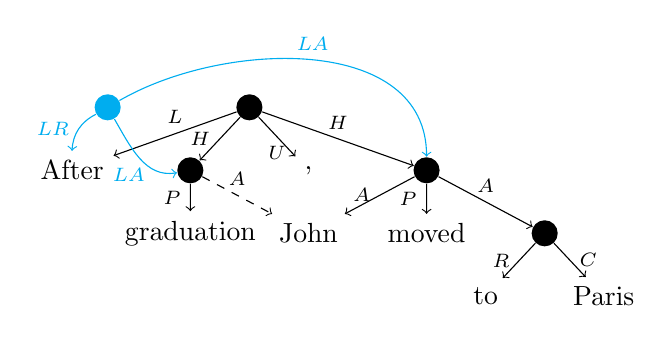
\begin{tikzpicture}[level distance=8mm, ->]
    \node (ROOT) [fill=black, circle] {}
      child {node (After) {After} edge from parent node[above] {\scriptsize $L$}}
      child {node (graduation) [fill=black, circle] {}
      {
        child {node {graduation} edge from parent node[left] {\scriptsize $P$}}
      } edge from parent node[left] {\scriptsize $H$} }
      child {node {,} edge from parent node[below] {\scriptsize $U$}}
      child {node (moved) [fill=black, circle] {}
      {
        child {node (John) {John} edge from parent node[left] {\scriptsize $A$}}
        child {node {moved} edge from parent node[left] {\scriptsize $P$}}
        child {node [fill=black, circle] {}
        {
          child {node {to} edge from parent node[left] {\scriptsize $R$}}
          child {node {Paris} edge from parent node[right] {\scriptsize $C$}}
        } edge from parent node[above] {\scriptsize $A$} }
      } edge from parent node[above] {\scriptsize $H$} }
      ;
    \draw[dashed,->] (graduation) to node [above] {\scriptsize $A$} (John);
    \node (LKG) at (-1.8,0) [fill=cyan, circle] {};
    \draw[bend right,color=cyan] (LKG) to node [auto, left] {\scriptsize $LR$} (After);
    \draw[color=cyan] (LKG) to[out=-60, in=190] node [below] {\scriptsize $LA\quad$} (graduation);
    \draw[color=cyan] (LKG) to[out=30, in=90] node [above] {\scriptsize $LA$} (moved);
  \end{tikzpicture}
  }\caption{UCCA \label{fig:original_example_ucca}}
\end{subfigure}}

\fbox{\begin{subfigure}{0.67\textwidth}
  \centering
  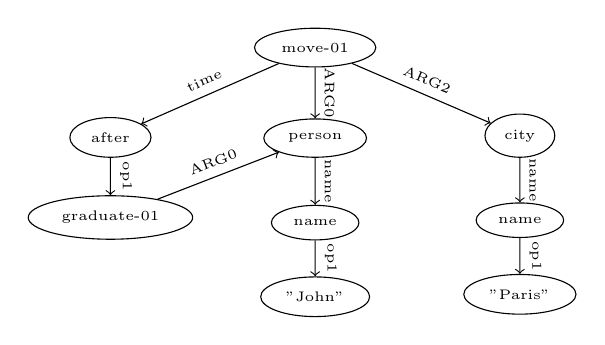
\begin{tikzpicture}[->,
      every node/.append style={sloped,anchor=south,auto=false,font=\tiny},
      level 1/.style={level distance=14mm,sibling distance=26mm},
      level 2/.style={level distance=13mm},
      level 3/.style={level distance=12mm}]
    \node (ROOT) [draw=black,ellipse] {move-01}
      child {node [draw=black,ellipse] {after}
      {
            child {node (graduation) [draw=black,ellipse] {graduate-01} edge from parent node {op1} }
      } edge from parent node {time} }
      child {node (John) [draw=black,ellipse] {person}
      {
        child {node [draw=black,ellipse] {name}
        {
            child {node [draw=black,ellipse] {"John"} edge from parent node {op1} }
        } edge from parent node {name} }
      } edge from parent node {ARG0} }
      child {node [draw=black,ellipse] {city}
      {
        child {node [draw=black,ellipse] {name}
        {
            child {node [draw=black,ellipse] {"Paris"} edge from parent node {op1} }
        } edge from parent node {name} }
      } edge from parent node {ARG2} }
      ;
      \draw (graduation) to node {ARG0} (John);
  \end{tikzpicture}
  \caption{AMR \label{fig:original_example_amr}}
\end{subfigure}}

\fbox{\begin{subfigure}{0.67\textwidth}
  \centering
    \begin{dependency}[text only label, label style={above}, font=\small]
    \begin{deptext}[column sep=.8em,ampersand replacement=\^]
    After \^ graduation \^ , \^ John \^ moved \^ to \^ Paris \\
    \end{deptext}
        \depedge[edge unit distance=1ex]{1}{2}{ARG2}
        \depedge[edge unit distance=1ex]{5}{4}{ARG1}
        \depedge[edge unit distance=1ex, edge end x offset=-2pt]{1}{5}{ARG1}
        \deproot[edge unit distance=1.5ex]{5}{top}
        \depedge[edge unit distance=2ex, edge start x offset=-1pt, edge end x offset=3pt]{5}{7}{ARG2}
        \depedge[edge unit distance=1ex, edge end x offset=5pt]{6}{5}{ARG1}
        \depedge[edge unit distance=1ex]{6}{7}{ARG2}
    \end{dependency}
  \caption{DM \label{fig:original_example_sdp}}
\end{subfigure}}

\fbox{\begin{subfigure}{0.67\textwidth}
  \centering
    \begin{dependency}[text only label, label style={above}, font=\small]
    \begin{deptext}[column sep=.8em,ampersand replacement=\^]
    After \^ graduation \^ , \^ John \^ moved \^ to \^ Paris \\
    \end{deptext}
        \depedge[edge unit distance=1ex]{2}{1}{case}
        \depedge[edge unit distance=1ex]{2}{3}{punct}
        \depedge[edge unit distance=1ex]{5}{4}{nsubj}
        \depedge[edge unit distance=1ex, edge end x offset=-2pt]{5}{2}{obl}
        \depedge[edge unit distance=1ex]{7}{6}{case}
        \deproot[edge unit distance=1.5ex]{5}{root}
        \depedge[edge unit distance=1.5ex]{5}{7}{obl}
    \end{dependency}
  \caption{UD \label{fig:original_example_uda}}
\end{subfigure}}


\caption{\label{fig:original_examplesa}
 Example graph for each task.
 Figure \ref{fig:original_example_ucca} presents a UCCA graph. The dashed edge is remote,
  while the blue node and its outgoing edges represent inter-Scene linkage.
  Pre-terminal nodes and edges are omitted for brevity. 
 Figure \ref{fig:original_example_amr} presents an AMR graph.
  Text tokens are not part of the graph, and must be matched to
  concepts and constants by alignment.
  Variables are represented by their concepts.
 Figure \ref{fig:original_example_sdp} presents a DM semantic dependency graph,
  containing multiple roots: ``After'', ``moved'' and ``to'',
  of which ``moved'' is marked as \textit{top}.
  Punctuation tokens are excluded from SDP graphs.
 Figure \ref{fig:original_example_uda} presents a UD tree.
  %Each word has exactly one head, and there is a single root.
  Edge labels express syntactic relations.}

\end{figure}


%%%%%%%%%%%%%%%%%%%%%%%%%%%%%%%%%%%%%%%%%%%%%%%%%%%%%%%%%%%%%%%%%%%%%%%%%%%%%%%%%
\section{Tackled Parsing Tasks}\label{sec:tasks}

In this section, we outline the parsing tasks we address.
We focus on representations that produce full-sentence analyses,
i.e., produce a graph covering all (content) words in the text, 
or the lexical concepts they evoke.
This contrasts with ``shallow'' semantic parsing,
primarily semantic role labeling
\cite[SRL;][]{gildea2002automatic,Palmer:05},
which targets argument structure phenomena using flat structures.
We consider four formalisms: UCCA, AMR, SDP and Universal Dependencies.
Figure~\ref{fig:original_examplesa} presents one sentence annotated in each scheme.
%annotating the sentence ``After graduation, John moved to Paris''.

%Although each of these tasks uses different graph structures,
%they all involve whole-sentence (or whole-paragraph) semantic analysis,
%and due to the structure of phenomena such as predicate-argument relations,
%require parsers that can handle non-projectivity (or discontinuity) and reentrancy, resulting in
%directed acyclic graphs (DAGs).\oa{maybe add a diagram or at least elaborate more on these like we
%did in the TUPA paper, with examples etc.}

\paragraph{Universal Conceptual Cognitive Annotation.}\label{sec:ucca}
UCCA \cite{abend2013universal} is a semantic representation whose main design principles
are ease of annotation, cross-linguistic applicability, and a modular architecture.
%of semantic distinctions.
UCCA represents the semantics of linguistic utterances
as directed acyclic graphs (DAGs), where terminal (childless) nodes
correspond to the text tokens, and non-terminal nodes to semantic units that participate
in some super-ordinate relation.
Edges are labeled, indicating the role of a child in the relation the parent represents.
Nodes and edges belong to one of several \textit{layers}, each corresponding
to a ``module'' of semantic distinctions.
UCCA's \textit{foundational layer} (the only layer for which annotated data exists)
mostly covers predicate-argument structure, semantic heads and inter-Scene relations.
%The \textit{linkage} layer covers relations between events, including temporal and discourse relations
%(exemplified by the gray node and its outgoing edges in Figure~\ref{fig:original_example_ucca}).

UCCA distinguishes \textit{primary} edges, corresponding 
to explicit relations, from \textit{remote} edges (appear dashed in
Figure~\ref{fig:original_example_ucca}) that allow for a unit to participate
in several super-ordinate relations.
Primary edges form a tree in each layer, whereas remote edges enable reentrancy, forming a DAG.
%As UCCA annotated data is currently fairly scarce (see \S\ref{sec:experimentsc}), 
%we hypothesize it will benefit from MTL, and consider it as our
%main task.

%%%%%%%%%%%%%%%%%%%%%%%%%%%%%%%%%%%%%%%%%%%%%%%%%%%%%%%%%%%%%%%%%%%%%%%%%%%%%5
\paragraph{Abstract Meaning Representation.}\label{sec:amr}

AMR \cite{banarescu2013abstract} is a semantic representation that encodes information about named entities, 
argument structure, semantic roles, word sense and co-reference.
AMRs are rooted directed graphs, in which both nodes and edges are labeled.
Most AMRs are DAGs, although cycles are permitted.

AMR differs from the other schemes we consider in that it does not anchor its graphs
in the words of the sentence (Figure~\ref{fig:original_example_amr}). Instead, AMR graphs
connect variables, concepts (from a pre-defined set) and constants (which may be strings or numbers).
Still, most AMR nodes are alignable to text tokens, a tendency used by AMR parsers,
which align a subset of the graph nodes to a subset of the text tokens (concept identification). In this work, we use pre-aligned AMR graphs.

Despite the brief period since its inception, AMR has been targeted by a number of works,
notably in two SemEval shared tasks \cite{may2016semeval,may2017semeval}.
To tackle its variety of distinctions and unrestricted graph structure,
AMR parsers often use specialized methods.
Graph-based parsers construct AMRs
by identifying concepts and scoring edges between them, either in a pipeline fashion
\cite{flanigan2014discriminative,artzi2015broad,pust2015parsing,foland2017abstract},
or jointly \cite{zhou2016amr}.
Another line of work %uses sequence-to-sequence models \cite{sutskever2014sequence},
trains machine translation models to convert strings into linearized AMRs
%treating AMR parsing as a machine translation model and linearizing the graph structure
\cite{barzdins2016riga,Gildea2017AddressingTD,Konstas2017NeuralAS,Buys2017RobustIN}.
Transition-based AMR parsers either 
use dependency trees as pre-processing, then mapping them into AMRs
\cite{wang-xue-pradhan:2015:ACL-IJCNLP,wang2015transition,wang-EtAl:2016:SemEval,goodman2016noise},
or use a transition system tailored to AMR parsing \cite{damonte-17,D17-1130}.
We differ from the above approaches in addressing AMR parsing 
using the same general DAG parser used for other schemes.


%%%%%%%%%%%%%%%%%%%%%%%%%%%%%%%%%%%%%%%%%%%%%%%%%%%%%%%%%%%%%%%%%%%%%%%%%%%%%5
\paragraph{Semantic Dependency Parsing.}\label{sec:sdp}

SDP uses a set of related representations, targeted in two recent SemEval shared tasks 
\cite{oepen2014semeval,oepen2015semeval}, and extended by \citet{oepen2016towards}.
They correspond to four semantic representation schemes, referred to as
DM, PAS, PSD and CCD, representing
predicate-argument relations between content words in a sentence.
All are based on semantic formalisms %whose annotation has been
converted into bilexical dependencies---directed graphs whose nodes are text tokens.
Edges are labeled, encoding semantic relations between the tokens.
Non-content tokens, such as punctuation,
are left out of the analysis (see Figure~\ref{fig:original_example_sdp}).
%but the sub-graph restricted to content-bearing tokens is connected.
Graphs containing cycles have been removed from the SDP datasets.

We use one of the representations
from the SemEval shared tasks: DM (DELPH-IN MRS), converted from 
DeepBank \cite{flickinger2012deepbank}, a corpus of hand-corrected parses from LinGO
ERG \cite{copestake2000open},
an HPSG \cite{pollard1994head}
using Minimal Recursion Semantics \cite{copestake2005minimal}.


%%%%%%%%%%%%%%%%%%%%%%%%%%%%%%%%%%%%%%%%%%%%%%%%%%%%%%%%%%%%%%%%
\paragraph{Universal Dependencies.}\label{sec:ud}
UD \cite{nivre2016universal,11234/1-2515} has quickly become
the dominant dependency scheme for
syntactic  annotation in many languages,
aiming for cross-linguistically consistent and coarse-grained treebank
annotation. Formally, UD uses bilexical trees, with edge labels 
representing syntactic relations between words.

We use UD as an auxiliary task,
inspired by previous work on joint syntactic and semantic parsing
(see \S\ref{sec:related_workc}).
%\cite{lluis2008joint,collobert2011natural,D15-1169,swayamdipta-EtAl:2016:CoNLL,swayamdipta2017frame}.
In order to reach comparable analyses cross-linguistically,
UD often ends up in annotation that is similar to the common practice
in semantic treebanks, such as linking content words to content words wherever possible.
Using UD further allows conducting experiments on languages other than English, 
for which AMR and SDP annotated data is not available (\S\ref{sec:experimentsc}).

In addition to basic UD trees, we use the \textit{enhanced++} UD graphs available for English,
which are generated by the Stanford CoreNLP converters
\cite{SCHUSTER16.779}.\footnote{\url{http://github.com/stanfordnlp/CoreNLP}}
These include additional and augmented relations between content words,
partially overlapping with the notion of remote edges in UCCA:
in the case of control verbs, for example, a direct relation is added in 
enhanced++ UD between the subordinated verb and its controller,
which is similar to the semantic schemes' treatment of this construction.


%%%%%%%%%%%%%%%%%%%%%%%%%%%%%%%%%%%%%%%%%%%%%%%%%%%%%%%%%%%%%%%%%%%%%%%%%%%%%%%%%%%%%%%%
\section{General Transition-based DAG Parser}\label{sec:modela}

All schemes considered in this work exhibit
reentrancy and discontinuity (or non-projectivity), to varying degrees.
In addition, UCCA and AMR contain non-terminal nodes.
To parse these graphs,
we extend TUPA \cite{hershcovich2017a}, 
a transition-based parser 
originally developed for UCCA,  as it
%is the only parser to our knowledge that
supports all these structural properties.
TUPA's transition system can yield any labeled DAG
whose terminals are anchored in the text tokens.
To support parsing into AMR, which uses graphs that are not anchored in the tokens,
 we take advantage of existing alignments of the graphs with the text
tokens during training (\S\ref{sec:formata}).

First used for projective syntactic dependency tree parsing \cite{Nivre03anefficient},
transition-based parsers have since been generalized to parse into many other
graph families, such as (discontinuous) constituency trees \cite[e.g., ][]{zhang2009transition,maier-lichte:2016:DiscoNLP},
and DAGs \cite[e.g.,][]{sagae2008shift,du-EtAl:2015:SemEval}. %ribeyre-villemontedelaclergerie-seddah:2014:SemEval,
Transition-based parsers apply \textit{transitions}
incrementally to an internal state defined by a buffer $B$ of remaining tokens 
and nodes, a stack $S$ of unresolved nodes, and a labeled graph $G$ of 
constructed nodes and edges.
When a terminal state is reached, the graph $G$ is the final output.
A classifier is used at each step to select the next transition, 
based on features that encode the current state.
%During training, an oracle converts the gold-standard annotations into
% training instances.




\subsection{TUPA's Transition Set}\label{sec:transition_set}

Given a sequence of tokens $w_1, \ldots, w_n$,
we predict a rooted graph $G$ whose terminals are the tokens.
Parsing starts with the root node on the stack,
and the input tokens in the buffer.

The TUPA transition set includes
the standard \textsc{Shift} and \textsc{Reduce} operations,
\textsc{Node$_X$} for creating a new non-terminal node and an $X$-labeled edge,
\textsc{Left-Edge$_X$} and \textsc{Right-Edge$_X$} to create a new primary $X$-labeled edge,
\textsc{Left-Remote$_X$} and \textsc{Right-Remote$_X$} to create a new remote $X$-labeled edge,
\textsc{Swap} to handle discontinuous nodes,
and \textsc{Finish} to mark the state as terminal.

Although UCCA contains nodes without any text tokens as descendants
(called \textit{implicit units}),
these nodes are infrequent and only cover 0.5\% of non-terminal nodes.
For this reason we follow previous work \cite{hershcovich2017a} and discard implicit units from
the training and evaluation,
and so do not include transitions for creating them.

In AMR, implicit units are considerably more common, as any unaligned concept
with no aligned descendents is implicit (about 6\% of the nodes).
Implicit AMR nodes usually result from alignment errors, or from abstract concepts
which have no explicit realization in the text \cite{buys2017oxford}.
We ignore implicit nodes when training on AMR as well.
TUPA also does not support node labels, 
which are ubiquitous in AMR but absent in UCCA structures (only edges are labeled in UCCA). 
We therefore only produce edge labels and not node labels when training on AMR.



%%%%%%%%%%%%%%%%%%%%%%%%%%%%%%%%%%%%%%%%%%%%%%%%%%%%%%%%%%%%%%%%%%%%%%%%%%%%%%%%%
\subsection{Transition Classifier}\label{sec:classifier}

To predict the next transition at each step,
we use a BiLSTM with embeddings as inputs,
followed by an MLP and a softmax layer for classification \cite{kiperwasser2016simple}.
The model is illustrated in Figure~\ref{fig:single_model}.
Inference is performed greedily,
and training is done with an oracle that yields the set of all optimal 
transitions at a given state (those that lead to a state from which the gold graph is still reachable).
Out of this set, the actual transition performed in training is the one
with the highest score given by the classifier,
which is trained to maximize the sum of log-likelihoods of all 
optimal transitions at each step.

\begin{figure}[H]\centering
   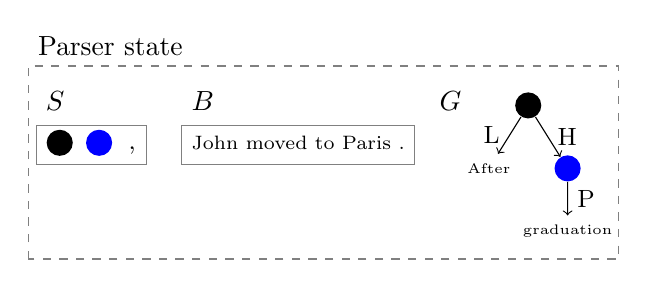
\begin{tikzpicture}[level distance=8mm, sibling distance=1cm]
   \node[anchor=west] at (0,1.5) {Parser state};
   \draw[color=gray,dashed] (0,-1.2) rectangle (7.5,1.25);
   \draw[color=gray] (.1,0) rectangle (1.5,.5);
   \node[anchor=west] at (.1,.8) {$S$};
   \node[fill=black, circle] at (.4,.275) {};
   \node[fill=blue, circle] at (.9,.275) {};
   \node[anchor=west] at (1.15,.175) {\small ,};
   \draw[color=gray] (1.95,0) rectangle (4.9,.5);
   \node[anchor=west] at (1.95,.8) {$B$};
   \node[anchor=west] at (1.95,.275) {\scriptsize John moved to Paris .};
   \node[anchor=west] at (5.1,.8) {$G$};
   \node[fill=black, circle] at (6.35,.75) {}
     child {node  {\tiny After} edge from parent [->] node[left] {\small L}}
     child {node [fill=blue, circle] {}
     {
       child {node {\tiny graduation} edge from parent [->] node[right] {\small P}}
     } edge from parent [->] node[right] {\small H} };
   \end{tikzpicture}
   
   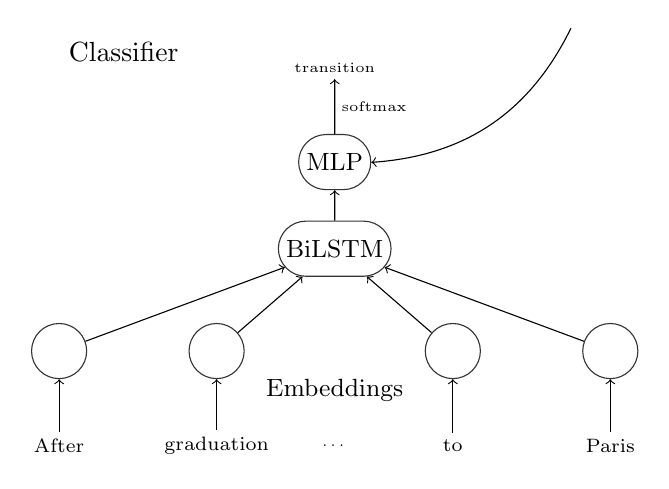
\begin{tikzpicture}[->]
   \node[anchor=west] at (0,6) {Classifier};
   \tiny
   \tikzstyle{main}=[rounded rectangle, minimum size=7mm, draw=black!80, node distance=12mm]
   \node[main] (specific) at (3.5,3.5) {\small BiLSTM};
   \node (embeddings) at (3.5,1.7) {\small Embeddings};
   \foreach \i/\word in {0/{After},2/{graduation},5/{to},7/{Paris}} {
       \node (x\i) at (\i,1) {\scriptsize \word};
       \node[main] (e\i) at (\i,2.2) {};
       \path (x\i) edge (e\i);
       \path (e\i) edge (specific);
   }
    \node (x4) at (3.5,1) {\ldots};
    \node[main] (mlp) at (3.5,4.6) {\small MLP};
    \path (specific) edge (mlp);
    \coordinate (state) at (6.5,6.3);
    \path (state) edge [bend left] (mlp);
    \node (transition) at (3.5,5.8) {transition};
    \path (mlp) edge node[right] {softmax} (transition);
   \end{tikzpicture}
\caption{Illustration of the TUPA model, adapted from \citet{hershcovich2017a}.
Top: parser state.
Bottom: BiLTSM architecture.}\label{fig:single_model}
\end{figure}


\begin{figure}[ht]\centering
\fbox{\begin{subfigure}{0.47\textwidth}
    \centering
    \scalebox{.95}{
    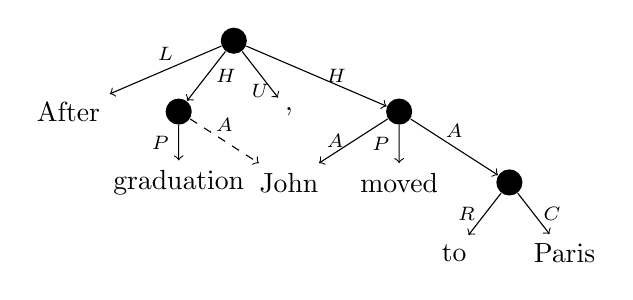
\begin{tikzpicture}[level distance=9mm, sibling distance=14mm, ->,
        every circle node/.append style={fill=black}]
      \tikzstyle{word} = [font=\rmfamily,color=black]
      \node (ROOT) [circle] {}
        child {node (After) [word] {After} edge from parent node[above] {\scriptsize $L$}}
        child {node (graduation) [circle] {}
        {
          child {node [word] {graduation} edge from parent node[left] {\scriptsize $P$}}
        } edge from parent node[right] {\scriptsize $H$} }
        child {node [word] {,} edge from parent node[below] {\scriptsize $U$}}
        child {node (moved) [circle] {}
        {
          child {node (John) [word] {John} edge from parent node[left] {\scriptsize $A$}}
          child {node [word] {moved} edge from parent node[left] {\scriptsize $P$}}
          child {node [circle] {}
          {
            child {node [word] {to} edge from parent node[left] {\scriptsize $R$}}
            child {node [word] {Paris} edge from parent node[right] {\scriptsize $C$}}
          } edge from parent node[above] {\scriptsize $A$} }
        } edge from parent node[right] {\scriptsize $H$} }
        ;
      \draw[dashed,->] (graduation) to node [above] {\scriptsize $A$} (John);
    \end{tikzpicture}}
  \caption{UCCA}
  \label{fig:converted_example_uccaa}
\end{subfigure}}

\fbox{\begin{subfigure}{0.47\textwidth}
  \centering
  \scalebox{.95}{
  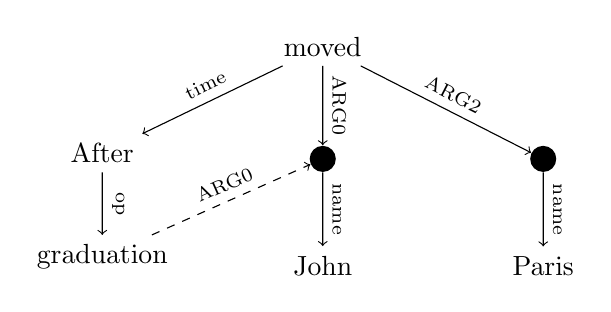
\begin{tikzpicture}[level distance=16mm, ->,
      every node/.append style={sloped,anchor=south,auto=false,font=\scriptsize},
      level 1/.style={sibling distance=28mm},
      level 2/.style={sibling distance=14mm},
      level 3/.style={sibling distance=12mm}]
    \tikzstyle{word} = [font=\rmfamily,color=black]
    \node (ROOT) [word] {moved}
      child {node [word] {After}
      {
            child {node (graduation) [word] {graduation} edge from parent node {op} }
      } edge from parent node {time} }
      child {node (John) [fill=black,circle] {}
      {
        child {node [word] {John} edge from parent node {name} }
      } edge from parent node {ARG0} }
      child {node [fill=black,circle] {}
      {
        child {node [word] {Paris} edge from parent node {name} }
      } edge from parent node {ARG2} }
      ;
      \draw[dashed] (graduation) to node {ARG0} (John);
  \end{tikzpicture}}
  \captionof{figure}{AMR}
  \label{fig:converted_example_amr}
\end{subfigure}}

\fbox{\begin{subfigure}{0.47\textwidth}
  \centering
  \scalebox{.95}{
  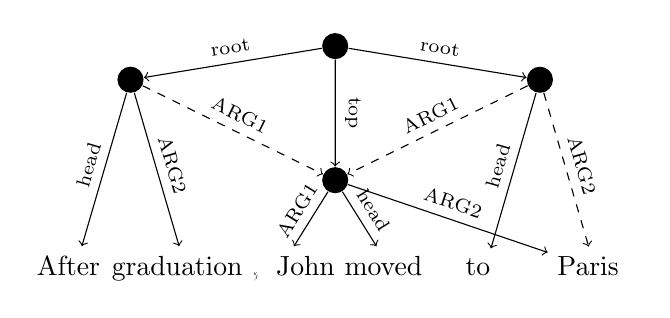
\begin{tikzpicture}[level distance=12mm, ->,
      every node/.append style={sloped,anchor=south,auto=false,font=\scriptsize},
      level 1/.style={sibling distance=26mm,level distance=6mm},
      level 2/.style={sibling distance=14mm,level distance=14mm}]
    \tikzstyle{word} = [font=\rmfamily,color=black]
    \node (ROOT) [fill=black,circle] {}
      child {node (after) [fill=black,circle] {}
      {
        child {node [draw=none] {}
        {
          child {node [word] (after_word) {After{\color{white}g}} edge from parent [draw=none]}
        } edge from parent [draw=none] }
        child {node [draw=none] {}
        {
          child {node [word] (graduation) {graduation ,} edge from parent [draw=none]}
        } edge from parent [draw=none] }
      } edge from parent node {root}}
      child {node [draw=none] {}
      {
        child {node (moved) [fill=black,circle] {}
        {
          child {node [word] {\quad{\color{white}g} John} edge from parent node {ARG1}}
          child {node [word] {moved{\color{white}g}} edge from parent node {head}}
        } edge from parent [draw=none] }
      } edge from parent [draw=none] }
      child {node (to) [fill=black,circle] {}
      {
        child {node [draw=none] {}
        {
            child {node [word] (to_word) {to{\color{white}g}} edge from parent [draw=none]}
          } edge from parent [draw=none] }
          child {node [draw=none] {}
        {
          child {node [word] (Paris) {Paris{\color{white}g}} edge from parent [draw=none]}
        } edge from parent [draw=none] }
      } edge from parent node {root}}
      ;
      \draw (ROOT) to node {top} (moved);
      \draw (after) to node {head} (after_word);
      \draw (after) to node {ARG2} (graduation);
      \draw[dashed] (after) to node {ARG1} (moved);
      \draw[dashed] (to) to node {ARG1} (moved);
      \draw (to) to node {head} (to_word);
      \draw (moved) to node {ARG2} (Paris);
      \draw[dashed] (to) to node {ARG2} (Paris);
  \end{tikzpicture}}
  \captionof{figure}{DM}
  \label{fig:converted_example_sdp}
\end{subfigure}}

\fbox{\begin{subfigure}{0.47\textwidth}
  \centering
  \scalebox{.95}{
  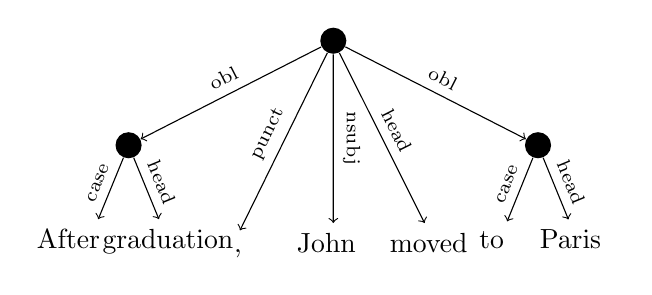
\begin{tikzpicture}[level distance=15mm, ->,
      every node/.append style={sloped,anchor=south,auto=false,font=\scriptsize},
      level 1/.style={sibling distance=13mm},
      level 2/.style={sibling distance=1cm}]
    \tikzstyle{word} = [font=\rmfamily,color=black]
    \node (ROOT) [fill=black,circle] {}
      child {node (after) [fill=black,circle] {}
      {
        child {node [word] {After{\color{white}g}\quad\quad} edge from parent node {case}}
        child {node [word] {\quad graduation\quad\quad} edge from parent node {head}}
      } edge from parent node {obl}}
      child {node {}
      {
        child {node [word] (comma) {\quad,{\color{white}g}} edge from parent [draw=none]}
      } edge from parent [draw=none]}
      child {node {}
      {
        child {node [word] (John) {John{\color{white}g}} edge from parent [draw=none]}
      } edge from parent [draw=none]}
      child {node {}
      {
        child {node [word] (moved) {moved{\color{white}g}} edge from parent [draw=none]}
      } edge from parent [draw=none]}
      child {node (to) [fill=black,circle] {}
      {
          child {node [word] {to{\color{white}g}} edge from parent node {case}}
          child {node [word] {Paris{\color{white}g}} edge from parent node {head}}
      } edge from parent node {obl}}
      ;
      \draw (ROOT) to node {punct} (comma);
      \draw (ROOT) to node {nsubj} (John);
      \draw (ROOT) to node {head} (moved);
  \end{tikzpicture}}
  \captionof{figure}{UD}\label{fig:converted_example_uda}
\end{subfigure}}

\caption{Graphs from Figure~\ref{fig:original_examplesa}, after conversion to  the unified DAG format
(with pre-terminals omitted: each terminal drawn in place of its parent).
Figure~\ref{fig:converted_example_uccaa} presents a converted UCCA graph.
Linkage nodes and edges are removed, but the original graph is otherwise preserved.
Figure~\ref{fig:converted_example_amr} presents a converted AMR graph, with
text tokens added according to the alignments.
Numeric suffixes of \textit{op} relations are removed,
and names collapsed.
Figure~\ref{fig:converted_example_sdp} presents a converted SDP graph (in the DM representation), with
intermediate non-terminal \textit{head} nodes introduced.
In case of reentrancy, an arbitrary reentrant edge is marked as remote.
Figure~\ref{fig:converted_example_uda} presents a converted UD graph.
As in SDP, intermediate non-terminals and \textit{head} edges are introduced.
While converted UD graphs form trees, enhanced++ UD graphs may not.}\label{fig:converted_examplesa}
\end{figure}


\paragraph{Features.}
We use the original TUPA features,
representing the words, POS tags, syntactic dependency relations, and previously predicted edge labels
for nodes in specific locations in the parser state.
In addition, for each token
we use embeddings representing the one-character prefix, three-character suffix,
shape (capturing orthographic features, e.g., ``Xxxx''),
and named entity type,\footnote{See Supplementary Material for a full listing of features.}
all provided by spaCy \cite{spacy2}.\footnote{\url{http://spacy.io}}
To the learned word vectors, we concatenate the 250K most frequent word vectors from fastText
\cite{bojanowski2016enriching},\footnote{\url{http://fasttext.cc}}
pre-trained over Wikipedia and updated during training.
%For AMR we add node label features according to gold node labels.


\paragraph{Constraints.}
As each annotation scheme has different constraints on the allowed graph structures,
we apply these constraints separately for each task.
During training and parsing, the relevant constraint set rules out some of the transitions
according to the parser state.
Some constraints are task-specific, others are generic.
For example, in UCCA, a terminal may only have one parent.
In AMR, a concept corresponding to a PropBank frame may only have 
the core arguments defined for the frame as children.
An example of a generic constraint is that stack nodes 
that have been swapped
should not be swapped again.\footnote{
 To implement this constraint, we define a \textit{swap index}
 for each node, assigned when the node is created.
 At initialization, only the root node and terminals exist.
 We assign the root a swap index of 0, and for each terminal, its
 position in the text (starting at 1).
 Whenever a node is created as a result of a \textsc{Node}
 transition, its swap index is the arithmetic
 mean of the swap indices of the stack top and buffer head.}


%%%%%%%%%%%%%%%%%%%%%%%%%%%%%%%%%%%%%%%%%%%%%%%%%%%%%%%%%%%%%%%%%%%%%%%%%%%%%%%%%%%%%%%%
\section{Unified DAG Format}\label{sec:formata}

To apply our parser to the four target tasks (\S\ref{sec:tasks}),
we convert them into a unified DAG format, which is inclusive enough to
allow representing any of the schemes with very little loss of information.\footnote{See
Supplementary Material for more conversion details.}

The format consists of a rooted DAG, where the tokens are the terminal nodes.
As in the UCCA format, edges are labeled (but not nodes),
and are divided into \textit{primary} and \textit{remote} edges,
where the primary edges form a tree (all nodes have at most one primary parent,
and the root has none).
Remote edges enable reentrancy, and thus together with primary edges
form a DAG.
Figure~\ref{fig:converted_examplesa} shows examples for converted graphs.
Converting UCCA into the unified format consists simply of removing linkage 
nodes and edges (see Figure~\ref{fig:converted_example_uccaa}), which were
also discarded by \citet{hershcovich2017a}.

\paragraph{Converting bilexical dependencies.}
To convert DM and UD into the unified DAG format,
we add a pre-terminal for each token,
and attach the pre-terminals according to the original dependency edges:
traversing the tree from the root down, for each head token we create a non-terminal
parent with the edge label {\it head},
and add the node's dependents as children of the created non-terminal node
(see Figures~\ref{fig:converted_example_sdp} and \ref{fig:converted_example_uda}).
Since DM allows multiple roots, we form a single root node, whose children
are the original roots. The added edges are labeled \textit{root}, where
top nodes are labeled \textit{top} instead.
In case of reentrancy, an arbitrary parent is marked as primary, and the rest as remote
(denoted as dashed edges in Figure~\ref{fig:converted_examplesa}).

\paragraph{Converting AMR.}
In the conversion from AMR, node labels are dropped.
Since alignments are not part of the AMR graph (see Figure~\ref{fig:converted_example_amr}),
we use automatic alignments (see \S\ref{sec:experimentsc}),
and attach each node with an edge to each of its aligned terminals.

%Since the order of AMR ordinal relations, such as \textit{op1}, \textit{op2},
%is annotated according to the order of text tokens,
%the numeric index is redundant and is thus removed.
%Numeric suffixes are kept when they are meaningful, e.g. in distinguishing between PropBank semantic
%roles (\textit{ARG[0-5]}).
Named entities in AMR are represented as a subgraph, whose \textit{name}-labeled root
has a child for each token in the name (see the two \textit{name} nodes in Figure~\ref{fig:original_example_amr}).
We collapse this subgraph into a single node whose children are the name tokens.


%%%%%%%%%%%%%%%%%%%%%%%%%%%%%%%%%%%%%%%%%%%%%%%%%%%%%%%%%%%%%%%%%%%%%%%%%%%%%%%%%%%%%%%%%%%%
\section{Multitask Transition-based Parsing}\label{sec:multitask}

Now that the same model can be applied to different tasks, 
we can train it in a multitask setting.
The fairly small training set available for UCCA (see \S\ref{sec:experimentsc})
makes MTL particularly appealing,
and we focus on it in this paper, treating AMR, DM and UD parsing as auxiliary tasks.

Following previous work, we share only some of the parameters
\cite{N16-1179,P16-2038,C16-1013,C16-1059,C16-1179,E17-1005,P17-1186,Peng-EtAl:2018:NAACL},
leaving task-specific
sub-networks as well.
Concretely, we keep the BiLSTM used by TUPA for the main task (UCCA parsing),
add a BiLSTM that is shared across all tasks,
and replicate the MLP (feedforward sub-network) for each task.
The BiLSTM outputs (concatenated for the main task) are
fed into the task-specific MLP (see Figure~\ref{fig:multi_model}).
Feature embeddings are shared across tasks.

\paragraph{Unlabeled parsing for auxiliary tasks.}
To simplify the auxiliary tasks and facilitate generalization \cite{E17-2026},
we perform unlabeled parsing for AMR, DM and UD,
while still predicting edge labels in UCCA parsing.
To support unlabeled parsing, we simply remove all labels from the
\textsc{Edge}, \textsc{Remote} and \textsc{Node} transitions output by the oracle.
This results in a much smaller number of transitions the classifier has to select from
(no more than 10, as opposed to 45 in labeled UCCA parsing),
allowing us to use no BiLSTMs and fewer dimensions and layers for task-specific MLPs
of auxiliary tasks (see \S\ref{sec:experimentsc}).
This limited capacity forces the network to use the shared parameters for all tasks,
increasing generalization \cite{E17-1005}.

\begin{figure}[H]\centering
   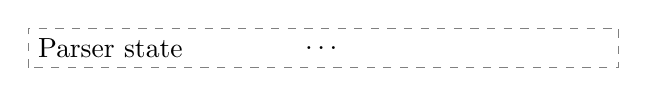
\begin{tikzpicture}
   \node[anchor=west] at (0,.25) {Parser state};
   \draw[color=gray,dashed] (0,0) rectangle (7.5,.5);
    \node (x4) at (3.75,0.25) {\ldots};
   \end{tikzpicture}
   
   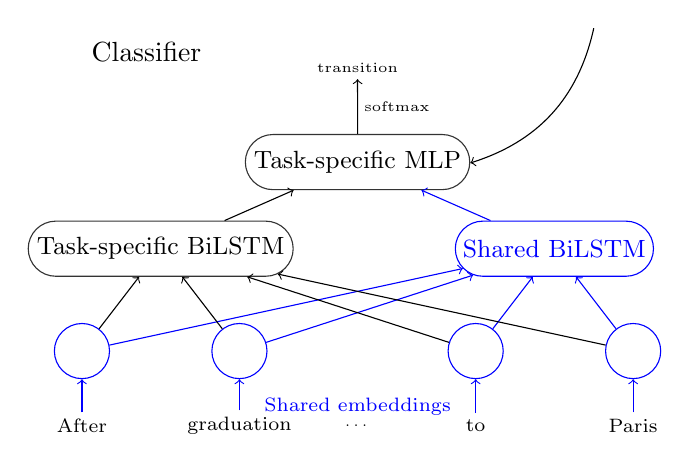
\begin{tikzpicture}[->]
   \node[anchor=west] at (0,6) {Classifier};
   \tiny
   \tikzstyle{main}=[rounded rectangle, minimum size=7mm, draw=black!80, node distance=12mm]
   \node[main] (specific) at (1,3.5) {\small Task-specific BiLSTM};
   \node[main,color=blue] (shared) at (6,3.5) {\small Shared BiLSTM};
   \node[color=blue] (embeddings) at (3.5,1.5) {\scriptsize Shared embeddings};
   \foreach \i/\word in {0/{After},2/{graduation},5/{to},7/{Paris}} {
       \node (x\i) at (\i,1.25) {\scriptsize \word};
       \node[main,color=blue] (e\i) at (\i,2.2) {};
       \path[color=blue] (x\i) edge (e\i);
       \path (e\i) edge (specific);
       \path[color=blue] (e\i) edge (shared);
   }
    \node (x4) at (3.5,1.25) {\ldots};
    \node[main] (mlp) at (3.5,4.6) {\small Task-specific MLP};
    \path (specific) edge (mlp);
    \path[color=blue] (shared) edge (mlp);
    \coordinate (state) at (6.5,6.3);
    \path (state) edge [bend left] (mlp);
    \node (transition) at (3.5,5.8) {transition};
    \path (mlp) edge node[right] {softmax} (transition);
   \end{tikzpicture}
   \caption{MTL model.
      Token representations are computed both by a task-specific and a shared BiLSTM.
      Their outputs are concatenated with the parser state embedding,
      identical to Figure~\ref{fig:single_model},
      and fed into the task-specific MLP for selecting the next transition.
      Shared parameters are shown in blue.}\label{fig:multi_model}
\end{figure}



\section{Experimental Setup}\label{sec:experimentsc}

We here detail a range of experiments to assess the value of MTL to UCCA parsing,
training the parser in single-task and multitask settings,
and evaluating its performance on the UCCA test sets in both in-domain and out-of-domain settings.

\begin{table*}[t]
\centering
\tiny
\setlength\tabcolsep{1.7pt}
\begin{tabular}{l|ccc|ccc||ccc|ccc||ccc|ccc}
& \multicolumn{6}{c||}{\footnotesize \bf English}
& \multicolumn{6}{c||}{\footnotesize \bf French}
& \multicolumn{6}{c}{\footnotesize \bf German} \\
\hline
& \multicolumn{3}{c|}{\footnotesize \bf {\#} tokens}
& \multicolumn{3}{c||}{\footnotesize \bf {\#} sentences}
& \multicolumn{3}{c|}{\footnotesize \bf {\#} tokens}
& \multicolumn{3}{c||}{\footnotesize \bf {\#} sentences}
& \multicolumn{3}{c|}{\footnotesize \bf {\#} tokens}
& \multicolumn{3}{c}{\footnotesize \bf {\#} sentences} \\
& \footnotesize \bf train & \footnotesize \bf dev & \footnotesize \bf test
& \footnotesize \bf train & \footnotesize \bf dev & \footnotesize \bf test
& \footnotesize \bf train & \footnotesize \bf dev & \footnotesize \bf test 
& \footnotesize \bf train & \footnotesize \bf dev & \footnotesize \bf test
& \footnotesize \bf train & \footnotesize \bf dev & \footnotesize \bf test
& \footnotesize \bf train & \footnotesize \bf dev & \footnotesize \bf test \\
\hline
\textbf{UCCA} &&&&&&&&&&&&&&&& \\
Wiki & 128444 & 14676 & 15313 & 4268 & 454 & 503 &&&&&&&&&&&& \\
20K &&& 12339 &&& 506 & 10047 & 1558 & 1324 & 413 & 67 & 67 & 79894 & 10059 & 42366 & 3429 & 561 & 2164 \\
\textbf{AMR} & \multicolumn{2}{l}{648950} && \multicolumn{2}{l}{36521} &&&&&&&&&&&&& \\
\textbf{DM} & \multicolumn{2}{l}{765025} && \multicolumn{2}{l}{33964} &&&&&&&&&&&&& \\
\textbf{UD} & \multicolumn{2}{l}{458277} && \multicolumn{2}{l}{17062} &&
\multicolumn{2}{l}{899163} && \multicolumn{2}{l}{32347} && \multicolumn{2}{l}{268145} && 13814
\end{tabular}
\caption{Number of tokens and sentences in the training, development and test sets
we use for each corpus and language.\label{tab:corpora}}
\end{table*}

\paragraph{Data.}

For UCCA, we use v1.2 of the English Wikipedia corpus \cite[\textit{Wiki};][]{abend2013universal},
with the standard train/dev/test split (see Table~\ref{tab:corpora}),
and the \textit{Twenty Thousand Leagues Under the Sea} corpora
\cite[\textit{20K};][]{sulem2015conceptual},
annotated in English, French and German.\footnote{\mbox{\url{http://github.com/huji-nlp/ucca-corpora}}}
For English and French we use 20K v1.0,
a small parallel corpus comprising the first five chapters of the book.
As in previous work \cite{hershcovich2017a}, we use the English part only as an out-of-domain test set.
We train and test on the French part using the standard split,
as well as the German corpus (v0.9),
which is a pre-release and still contains a considerable amount of noisy annotation.
Tuning is performed on the respective development sets.

For AMR, we use LDC2017T10, identical to the dataset targeted in SemEval 2017
\cite{may2017semeval}.\footnote{\mbox{\url{http://catalog.ldc.upenn.edu/LDC2017T10}}}
For SDP, we use the DM representation from the SDP 2016 dataset
\cite{oepen2016towards}.\footnote{\url{http://sdp.delph-in.net/osdp-12.tgz}}
For Universal Dependencies, we use all English, French and German treebanks from UD v2.1
\cite{11234/1-2515}.\footnote{\url{http://hdl.handle.net/11234/1-2515}}
We use the enhanced++ UD representation \cite{SCHUSTER16.779} in our English experiments,
henceforth referred to as UD$^{++}$.
We use only the AMR, DM and UD training sets from standard splits.

While UCCA is annotated over Wikipedia and over a literary corpus,
the domains for AMR, DM and UD are blogs, news, emails, reviews, and Q\&A.
This domain difference between training and test is particularly challenging (see \S\ref{sec:discussionc}).
Unfortunately, none of the other schemes have available annotation over Wikipedia text.

\paragraph{Settings.}

We explore the following settings: 
(1) in-domain setting in English, training and testing on Wiki;
(2) out-of-domain setting in English, training on Wiki and testing on 20K;
(3) French in-domain setting, where available training dataset is small,
training and testing on 20K;
(4) German in-domain setting on 20K, with somewhat noisy annotation.
For MTL experiments, we use unlabeled AMR, DM and UD$^{++}$ parsing as auxiliary tasks in English,
and unlabeled UD parsing in French and German.\footnote{We did not use AMR, DM or UD$^{++}$ in French
and German, as these are only available in English.}
We also report baseline results training only the UCCA training sets.


\paragraph{Training.}

We create a unified corpus for each setting, shuffling all sentences from relevant datasets together,
but using only the UCCA development set $F_1$ score as the early stopping criterion.
In each training epoch, we use the same number of examples from each task---the
UCCA training set size.
Since training sets differ in size, we sample this many sentences from each one.
The model is implemented using DyNet \cite{neubig2017dynet}.\footnote{\url{http://dynet.io}}


\begin{table}[h]
\centering
\small
\begin{tabular}{l|c|ccccc}
&& \multicolumn{3}{c}{\bf Multitask} \\ 
\bf Hyperparameter &  \bf Single & \bf Main & \bf Aux & \bf Shared \\
\hline
Pre-trained word dim. & 300 &&& 300 \\
Learned word dim. & 200 &&& 200 \\
POS tag dim. & 20 &&& 20 \\
Dependency relation dim. & 10 &&& 10 \\
Named entity dim. & 3 &&& 3 \\
Punctuation dim. & 1 &&& 1 \\
Action dim. & 3 &&& 3 \\
Edge label dim. & 20 & 20 \\
\hline
MLP layers & 2 & 2 & 1 \\
MLP dimensions & 50 & 50 & 50 \\
BiLSTM layers & 2 & 2 & & 2 \\
BiLSTM dimensions & 500 & 300 & & 300
\end{tabular}
\caption{Hyperparameter settings.
Middle column shows hyperparameters used for the single-task architecture,
described in \S\ref{sec:classifier}, and
right column for the multitask architecture,
described in \S\ref{sec:multitask}.
\textbf{Main} refers to parameters specific to the main task---UCCA parsing
(task-specific MLP and BiLSTM, and edge label embedding),
\textbf{Aux} to parameters specific to each auxiliary task
(task-specific MLP, but no edge label embedding since the tasks are unlabeled),
and \textbf{Shared} to parameters shared among all tasks
(shared BiLSTM and embeddings).\label{tab:hyperparams}}
\end{table}


\paragraph{Hyperparameters.}

We initialize embeddings randomly.
We use dropout \cite{srivastava2014dropout} between MLP layers, and recurrent dropout
\cite{NIPS2016_6241} between BiLSTM layers, both with $p=0.4$.
We also use word ($\alpha=0.2$), tag ($\alpha=0.2$) and dependency relation ($\alpha=0.5$) dropout
\cite{kiperwasser2016simple}.\footnote{In training, the embedding for a feature value $w$ is
replaced with a zero vector with a probability of $\frac{\alpha}{\#(w)+\alpha}$,
where $\#(w)$ is the number of occurrences of $w$ observed.}
In addition, we use a novel form of dropout, \textit{node dropout}:
with a probability of 0.1 at each step, all features associated with a single
node in the parser state are replaced with zero vectors.
For optimization we use a minibatch size of 100, decaying all weights by $10^{-5}$ at each update,
and train with stochastic gradient descent for $N$ epochs with a learning
rate of 0.1, followed by AMSGrad \cite{j.2018on} for $N$ epochs with
$\alpha=0.001,\beta_1=0.9$ and $\beta_2=0.999$.
We use $N=50$ for English and German, and $N=400$ for French.
We found this training strategy better than using only one of the optimization methods,
similar to findings by \citet{keskar2017improving}.
We select the epoch with the best average labeled $F_1$ score on the
UCCA development set.
Other hyperparameter settings are listed in Table~\ref{tab:hyperparams}.


\paragraph{Evaluation.}

We evaluate on UCCA using labeled precision, recall and $F_1$ 
on primary and remote edges,
following previous work \cite{hershcovich2017a}.
Edges in predicted and gold graphs are matched by terminal yield and label.
Significance testing of improvements over the single-task model is done
by the bootstrap test \cite{berg2012empirical}, with $p<0.05$.

%\subsection{Ensembling}
%
%During inference, we use Product of Experts \cite[PoE; ][]{hinton2002training} to combine the predictions
%of three models trained in the same setting, but with different random seeds. The transition selected is
%\[
%\argmax_{t\in T}\sum_{i=1}^3\big[\log(\mathrm{softmax}(m_i(s)))\big]_t
%\]
%where $T$ is the set of possible transitions, $m_i$ are the combined models, and $s$ is the current state.
%
%In order to ensemble multitask models, we combine models trained with the same auxiliary task.
%Another alternative is to combine models trained with different auxiliary tasks.\oa{don't write about alternatives,
%but rather on what we actually do}
%This provides greater variability between the combined models.



\section{Results}\label{sec:resultsb}


\begin{table}[t]
\centering
\small
\begin{tabular}{l|lll|lll}
& \multicolumn{3}{c|}{\footnotesize \bf Primary} & \multicolumn{3}{c}{\footnotesize \bf Remote} \\
& \footnotesize \textbf{LP} & \footnotesize \textbf{LR} & \footnotesize \textbf{LF}
& \footnotesize \textbf{LP} & \footnotesize \textbf{LR} & \footnotesize \textbf{LF} \\
\hline
\multicolumn{4}{l|}{\small \bf English (in-domain)} & \\
\footnotesize HAR17
& 74.4 & 72.7 & 73.5 & 47.4 & 51.6 & 49.4 \\
\footnotesize Single
& 74.4 & 72.9 & 73.6 & 53 & 50 & 51.5 \\
\cline{1-1}
%\small \bf Multitask &&& \\
\footnotesize AMR
& 74.7 & 72.8 & 73.7 & 48.7$\star$ & 51.1 & 49.9 \\
\footnotesize DM
& 75.7$\star$ & 73.9$\star$ & 74.8$\star$ & 54.9 & 53 & \textbf{53.9} \\
\footnotesize UD$^{++}$
& 75$\star$ & 73.2 & 74.1$\star$ & 49 & 52.7 & 50.8 \\
\footnotesize AMR + DM
& 75.6$\star$ & 73.9$\star$ & 74.7$\star$ & 49.9 & 53 & 51.4 \\
\footnotesize AMR + UD$^{++}$
& 74.9 & 72.7 & 73.8 & 47.1 & 50 & 48.5 \\
\footnotesize DM + UD$^{++}$
& 75.9$\star$ & 73.9$\star$ & \textbf{74.9}$\star$ & 48 & 54.8 & 51.2 \\
\footnotesize All
& 75.6$\star$ & 73.1 & 74.4$\star$ & 50.9 & 53.2 & 52
\end{tabular}
\caption{
Labeled precision, recall and $F_1$ (in~\%) for primary and remote edges,
on the \textbf{Wiki} test set.
$\star$~indicates significantly better than \textit{Single}.
HAR17: \citet{hershcovich2017a}.}\label{tab:id_results}
\end{table}


\begin{table}[t]
\centering
\small
\begin{tabular}{l|lll|lll}
& \multicolumn{3}{c|}{\footnotesize \bf Primary} & \multicolumn{3}{c}{\footnotesize \bf Remote} \\
& \footnotesize \textbf{LP} & \footnotesize \textbf{LR} & \footnotesize \textbf{LF}
& \footnotesize \textbf{LP} & \footnotesize \textbf{LR} & \footnotesize \textbf{LF} \\
\hline
\multicolumn{4}{l|}{\small \bf English (out-of-domain)} & \\
\footnotesize HAR17
& 68.7 & 68.5 & 68.6 & 38.6 & 18.8 & 25.3 \\
\footnotesize Single
& 69 & 69 & 69 & 41.2 & 19.8 & 26.7 \\
\cline{1-1}
%\small \bf Multitask &&& \\
\footnotesize AMR
& 69.5 & 69.5 & 69.5 & 42.9 & 20.2 & 27.5 \\
\footnotesize DM
& 70.7$\star$ & 70.7$\star$ & 70.7$\star$ & 42.7 & 18.6 & 25.9 \\
\footnotesize UD$^{++}$
& 69.6 & 69.8$\star$ & 69.7 & 41.4 & 22 & 28.7 \\
\footnotesize AMR + DM
& 70.7$\star$ & 70.2$\star$ & 70.5$\star$ & 45.8 & 19.4 & 27.3 \\
\footnotesize AMR + UD$^{++}$
& 70.2$\star$ & 69.9$\star$ & 70$\star$ & 45.1 & 21.8 & 29.4 \\
\footnotesize DM + UD$^{++}$
& 70.8$\star$ & 70.3$\star$ & 70.6$\star$ & 41.6 & 21.6 & 28.4 \\
\footnotesize All
& 71.2$\star$ & 70.9$\star$ & \textbf{71}$\star$ & 45.1 & 22 & \textbf{29.6} \\
\hline
\multicolumn{4}{l|}{\small \bf French (in-domain)} & \\
\small Single & 68.2 & 67 & 67.6 & 26 & \enskip 9.4 & 13.9 \\
\small UD & 70.3 & 70$\star$ & \textbf{70.1}$\star$ & 43.8 & 13.2 & 20.3 \\
\hline
\multicolumn{4}{l|}{\small \bf German (in-domain)} & \\
\small Single & 73.3 & 71.7 & 72.5 & 57.1 & 17.7 & 27.1 \\
\small UD & 73.7$\star$ & 72.6$\star$ & \textbf{73.2}$\star$ & 61.8 & 24.9$\star$ & \textbf{35.5}$\star$
\end{tabular}
\caption{
Labeled precision, recall and $F_1$ (in~\%) for primary and remote edges,
on the \textbf{20K} test sets.
$\star$~indicates significantly better than \textit{Single}.
HAR17: \citet{hershcovich2017a}.}\label{tab:ood_results}
\end{table}

Table~\ref{tab:id_results} presents our results on the English in-domain Wiki test set.
MTL with all auxiliary tasks and their combinations improves the primary $F_1$ score over
the single task baseline. In most settings the improvement is statistically significant.
Using all auxiliary tasks contributed less than just DM and UD$^{++}$,
the combination of which yielded the best scores yet in in-domain UCCA parsing,
with 74.9\% $F_1$ on primary edges.
Remote $F_1$ is improved in some settings, but due to the relatively small number of remote
edges (about 2\% of all edges), none of the differences is significant.
Note that our baseline single-task model (\textit{Single})
is slightly better than the current state-of-the-art \cite[HAR17;][]{hershcovich2017a},
due to the incorporation of additional features (see \S\ref{sec:classifier}).

Table~\ref{tab:ood_results} presents our experimental results on the 20K corpora in the three languages.
For English out-of-domain, improvements from using MTL are even more marked. 
Moreover, the improvement is largely additive: the best model, using all three auxiliary tasks (\textit{All}),
yields an error reduction of 2.9\%. Again, the single-task baseline is slightly better than HAR17.




The contribution of MTL is also apparent in French and German in-domain parsing:
3.7\% error reduction in French
(having less than 10\% as much UCCA training data as English)
and 1\% in German, where the training set is comparable in size to the English one,
but is noisier (see~\S\ref{sec:experimentsc}).
The best MTL models are significantly better than single-task models,
demonstrating that even a small training set for the main task may suffice,
given enough auxiliary training data (as in French).





\section{Discussion}\label{sec:discussionc}

\paragraph{Quantifying the similarity between tasks.}
Task similarity is an important factor in MTL success
\cite{E17-2026,E17-1005}.
In our case, the main and auxiliary tasks are annotated on different corpora
from different domains (\S\ref{sec:experimentsc}), and
the target representations vary both in form and in content.
%We found that the combination of many different domains therefore benefits domain
%adaptation even without auxiliary data from the target domain,
%in accordance with previous work \cite{Finkel2009JointPA}.

To quantify the domain differences, we follow \citet{Plank2011EffectiveMO} and measure the L1 distance 
between word distributions in the English training sets and 20K test set
(Table~\ref{tab:domain_sim}).
All auxiliary training sets are more similar to 20K than Wiki is, which may
contribute to the benefits observed on the English 20K test set.


\begin{table}[t]
\centering
\small
\begin{tabular}{l|cccc}
& \footnotesize 20K & \footnotesize AMR & \footnotesize DM & \footnotesize UD \\
\hline
\footnotesize Wiki & 1.047 & 0.895 & 0.913 & 0.843 \\
\footnotesize 20K && 0.949 & 0.971 & 0.904 \\
\footnotesize AMR &&& 0.757 & 0.469 \\
\footnotesize DM &&&& 0.754
\end{tabular}
\caption{L1 distance between dataset word distributions,
quantifying domain differences in English (low is similar).\label{tab:domain_sim}}
\end{table}


\begin{table}[t]
\centering
\small
\begin{tabular}{l|lll|lll}
& \multicolumn{3}{c|}{\footnotesize \bf Primary} & \multicolumn{3}{c}{\footnotesize \bf Remote} \\
& \footnotesize \textbf{UP} & \footnotesize \textbf{UR} & \footnotesize \textbf{UF}
& \footnotesize \textbf{UP} & \footnotesize \textbf{UR} & \footnotesize \textbf{UF} \\
\hline
AMR & 53.8 & 15.6 & 24.2 & \enskip 7.3 & \enskip 5.5 & \enskip 6.3 \\
DM & 65 & 49.2 & 56 & \enskip 7.4 & 65.9 & 13.3 \\
UD$^{++}$ & 82.7 & 84.6 & 83.6 & 12.5 & 12.7 & 12.6
\end{tabular}
\caption{Unlabeled $F_1$ scores between the representations of the same English sentences (from PTB WSJ), converted to the unified DAG format, and annotated UCCA graphs.\label{tab:common}}
\end{table}

As a measure of the formal similarity of the different schemes to UCCA,
we use unlabeled $F_1$ score evaluation on both primary and remote edges (ignoring edge labels).
To this end, we annotated 100 English sentences from Section 02 of the Penn Treebank Wall Street Journal
(PTB WSJ).
Annotation was carried out by a single expert UCCA annotator,
and is publicly available.\footnote{\url{http://github.com/danielhers/wsj}}
These sentences had already been annotated by the AMR, DM and PTB schemes,\footnote{We
convert the PTB format to UD$^{++}$ v1 using Stanford CoreNLP,
and then to UD v2 using Udapi: \url{http://github.com/udapi/udapi-python}.}
and we convert their annotation to the unified DAG format.

Unlabeled $F_1$ scores between the UCCA graphs and those converted from AMR, DM and UD$^{++}$
are presented in Table~\ref{tab:common}.
UD$^{++}$ is highly overlapping with UCCA, while DM less so, and AMR even less
(cf. Figure~\ref{fig:converted_examplesa}). 

Comparing the average improvements resulting from adding each of the tasks as auxiliary
(see \S\ref{sec:resultsb}), we find 
AMR the least beneficial, UD$^{++}$ second, and DM the most beneficial,
in both in-domain and out-of-domain settings.
This trend is weakly correlated with the formal similarity between the tasks
(as expressed in Table~\ref{tab:common}), but weakly negatively correlated with the word distribution similarity scores (Table~\ref{tab:domain_sim}).
We conclude that other factors should be taken into account to fully explain this effect,
and propose to address this in future work through controlled experiments, where corpora of the same
domain are annotated with the various formalisms and used as training data for MTL.

%However, due to the deep model architecture (\S\ref{sec:multitask}),
%generalizations useful to all tasks (e.g., lexical) may be shared,
%even if not expressed directly in nodes and edges.
%These findings suggest the diversity of domains may have as important an effect on parsing performance, as the diversity of formalisms. 


\paragraph{AMR, SDP and UD parsing.} 
Evaluating the full MTL model (\textit{All}) on the unlabeled auxiliary tasks yielded
64.7\% unlabeled Smatch $F_1$ \cite{cai2013smatch} on the AMR development set,
when using oracle concept identification
(since the auxiliary model does not predict node labels),
27.2\% unlabeled $F_1$ on the DM development set,
and 4.9\% UAS on the UD development set.
These poor results reflect the fact that model selection was based on the score
on the UCCA development set, and that the model parameters dedicated to auxiliary tasks were
very limited (to encourage using the shared parameters).
However, preliminary experiments using our approach produced
promising results on each of the tasks' respective English development sets,
when treated as a single task:
67.1\% labeled Smatch $F_1$ on AMR
(adding a transition for implicit nodes and classifier for node labels),
79.1\% labeled $F_1$ on DM,
and 80.1\% LAS $F_1$ on UD.
For comparison, the best results on these datasets are 70.7\%, 91.2\% and 82.2\%, respectively
\cite{foland2017abstract,Peng-EtAl:2018:NAACL,K17-3002}.



\section{Conclusion}\label{sec:conclusionb}

We demonstrate that semantic parsers can leverage a range of 
semantically and syntactically annotated data, to improve their performance.
Our experiments show that MTL improves UCCA parsing,
using AMR, DM and UD parsing as auxiliaries.
We propose a unified DAG representation, 
construct protocols for converting these schemes into the unified format,
and generalize a transition-based DAG parser to support all these tasks,
allowing it to be jointly trained on them.
%While the machine learning techniques we use are not novel,
%our contribution is in allowing these models to learn from
%significantly different tasks.

%A natural question is whether our method can benefit AMR, DM or UD parsing.
While we focus on UCCA in this work, our parser is capable of parsing any
scheme that can be represented in the unified DAG format,
and preliminary results on AMR, DM and UD are promising (see~\S\ref{sec:discussionc}).
Future work will investigate whether a single
algorithm and architecture can be competitive on all of these parsing tasks,
an important step towards a joint many-task model for semantic parsing.


%%%%%%%%%%%%%%%%%%%%%%%%%%%%%%%%%%%%%%%%%%%%%%%%%%%%%%%%%%%%%%%
\section*{Acknowledgments}

This work was supported by the Israel Science Foundation (grant no. 929/17),
by the HUJI Cyber Security Research Center
in conjunction with the Israel National Cyber Bureau in the Prime Minister's Office,
and by the Intel Collaborative Research Institute for Computational Intelligence (ICRI-CI).
The first author was supported by a fellowship from the
Edmond and Lily Safra Center for Brain Sciences.
We thank Roi Reichart, Rotem Dror
and the anonymous reviewers for their helpful comments.

%
% File udst2018.tex

\chapter{Universal Dependency Parsing with a General Transition-Based DAG Parser (Published in CoNLL 2018 Shared Task)}

\subsubsection*{Daniel Hershcovich$^{1,2}$, Omri Abend$^2$ and Ari Rappoport$^2$ \\
  $^1$The Edmond and Lily Safra Center for Brain Sciences \\
  $^2$School of Computer Science and Engineering \\
  Hebrew University of Jerusalem \\
  \texttt{\{danielh,oabend,arir\}@cs.huji.ac.il}  
}

\section*{Abstract}
This paper presents our experiments with applying TUPA to the CoNLL 2018 UD shared task. TUPA is a general neural transition-based DAG parser, which we use to present the first experiments on recovering enhanced dependencies as part of the general parsing task. TUPA was designed for parsing UCCA, a cross-linguistic semantic annotation scheme, exhibiting reentrancy, discontinuity and non-terminal nodes. By converting UD trees and graphs to a UCCA-like DAG format, we train TUPA almost without modification on the UD parsing task. The generic nature of our approach lends itself naturally to multitask learning.  
Our code is available at \url{https://github.com/CoNLL-UD-2018/HUJI}.

\section{Introduction}\label{sec:introduction}

In this paper, we present the HUJI submission to the CoNLL 2018 shared task
on Universal Dependency parsing \cite{conll2018UDSToverview}.
We focus only on parsing, using the baseline system, UDPipe 1.2
\cite{udpipe,udpipe:2017}
for tokenization, sentence splitting, part-of-speech tagging and morphological tagging.

Our system is based on TUPA \cite[see \S\ref{sec:model}]{hershcovich2017a,hershcovich2018multitask},
a transition-based UCCA parser.
UCCA \cite[Universal Conceptual Cognitive Annotation;][]{abend2013universal} is a
cross-linguistic semantic annotation scheme, representing events, participants,
attributes and relations in a directed acyclic graph (DAG) structure.
UCCA allows reentrancy to support argument sharing,
discontinuity (corresponding to non-projectivity in dependency formalisms)
and non-terminal nodes (as opposed to dependencies, which are bi-lexical).
To parse Universal Dependencies \cite{nivre2016universal}
using TUPA, we employ a bidirectional conversion protocol to represent
UD trees and graphs in a UCCA-like unified DAG format (\S\ref{sec:format}).


\paragraph{Enhanced dependencies.}
Our method treats \textit{enhanced dependencies}\footnote{\url{http://universaldependencies.org/u/overview/enhanced-syntax.html}}
as part of the dependency graph, providing the first approach, to our knowledge,
for supervised learning of enhanced UD parsing.
Due to the scarcity of enhanced dependencies in UD treebanks,
previous approaches \cite{SCHUSTER16.779,reddy2017universal} have attempted to recover them
using language-specific rules.
Our approach attempts to learn them from data:
while only a few UD treebanks contain any enhanced dependencies,
similar structures are an integral part of UCCA and its annotated corpora
(realized as reentrancy by remote edges; see \S\ref{sec:format}),
and TUPA supports them as a standard feature.

As their annotation in UD is not yet widespread and standardized,
enhanced dependencies are \textit{not included}
in the evaluation metrics for UD parsing,
and so TUPA's ability to parse them is not reflected in the official
shared task scores.
However, we believe these enhancements, representing
case information, elided predicates,
and shared arguments due to conjunction, control, raising
and relative clauses,
provide richer information to downstream semantic applications,
making UD better suited for text understanding.
We propose an evaluation metric specific to enhanced dependencies,
\textit{enhanced~LAS} (\S\ref{sec:enhanced_results}),
and use it to evaluate our method.


%%%%%%%%%%%%%%%%%%%%%%%%%%%%%%%%%%%%%%%%%%%%%%%%%%%%%%%%%%%%%%%%%%%%%%%%%%%%%%%%%%%%%%%%

\begin{figure}[ht]
\fbox{\begin{subfigure}{0.47\textwidth}
    \centering
    \scalebox{.95}{
    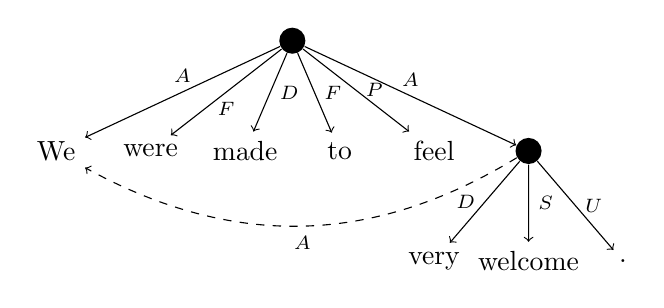
\begin{tikzpicture}[level distance=14mm,sibling distance=12mm, ->,
        every circle node/.append style={fill=black}]
      \tikzstyle{word} = [font=\rmfamily,color=black]
      \node (ROOT) [circle] {}
        child {node (We) [word] {We} edge from parent node[above] {\scriptsize  $A$}}
        child {node [word] {were} edge from parent node[below] {\scriptsize $F$}}
        child {node [word] {made} edge from parent node[right] {\scriptsize $D$}}
        child {node [word] {to} edge from parent node[right] {\scriptsize $F$}}
        child {node [word] {feel} edge from parent node[right] {\scriptsize $P$}}
        child {node (verywelcome) [circle] {}
        {
          child {node [word] {very} edge from parent node[left] {\scriptsize $D$}}
          child {node [word] {welcome} edge from parent node[right] {\scriptsize $S$}}
          child {node [word] {.} edge from parent node[right] {\scriptsize $U$}}
        } edge from parent node[above] {\scriptsize $A$} }
      ;
      \draw[dashed,->,bend left] (verywelcome) to node [below] {\scriptsize $A$} (We);
    \end{tikzpicture}}
  \caption{Example UCCA graph.}
  \label{fig:converted_example_ucca}
\end{subfigure}}
\fbox{\begin{subfigure}{0.57\textwidth}
  \centering
    \begin{dependency}[text only label, label style={above}, font=\small]
    \begin{deptext}[column sep=.5em,ampersand replacement=\^]
    We \^ were \^ made \^ to \^ feel \^ very \^ welcome \^ . \\
    \end{deptext}
        \depedge[edge start x offset=1pt]{3}{1}{nsubj:pass}
        \depedge[edge below,dashed,edge unit distance=.65ex,edge end x offset=2pt]{5}{1}{nsubj:xsubj}
        \depedge[edge below,dashed,edge unit distance=.8ex,edge end x offset=-1pt]{7}{1}{nsubj:xsubj}
        \depedge{3}{2}{aux:pass}
        \deproot[edge unit distance=3ex]{3}{root}
        \depedge{5}{4}{mark}
        \depedge{3}{5}{xcomp}
        \depedge{7}{6}{advmod}
        \depedge{5}{7}{xcomp}
        \depedge[edge unit distance=2ex,edge start x offset=-1pt]{3}{8}{punct}
    \end{dependency}
  \caption{\label{fig:original_examples}Example UD graph.}
\end{subfigure}}
\fbox{\begin{subfigure}{0.47\textwidth}
  \centering
  \scalebox{.95}{
    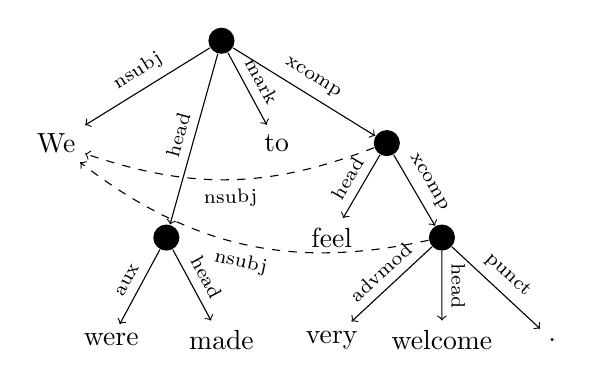
\begin{tikzpicture}[sibling distance=14mm, ->,
        every circle node/.append style={fill=black},
        level 1/.style={level distance=13mm},
        level 2/.style={level distance=12mm},
        level 3/.style={level distance=13mm}]
      \tikzstyle{word} = [font=\rmfamily,color=black]
      \node (ROOT) [circle] {}
        child {node (We) [word] {We} edge from parent node[midway,above,sloped] {\scriptsize nsubj}}
        child {node {}
        {
	        child {node (weremade) [circle] {}
	        {
	          child {node [word] {were} edge from parent node[midway,above,sloped] {\scriptsize aux}}
	          child {node [word] {made} edge from parent node[midway,above,sloped] {\scriptsize head}}
	        } edge from parent [draw=none]}
        } edge from parent [draw=none]}
        child {node [word] {to} edge from parent node[midway,above,sloped] {\scriptsize mark}}
        child {node (feelverywelcome) [circle] {}
        {
          child {node [word] {feel} edge from parent node[midway,above,sloped] {\scriptsize head}}
          child {node (verywelcome) [circle] {}
          {
            child {node [word] {very} edge from parent node[midway,above,sloped] {\scriptsize advmod}}
            child {node [word] {welcome} edge from parent node[midway,above,sloped] {\scriptsize head}}
            child {node [word] {.} edge from parent node[midway,above,sloped] {\scriptsize punct}}
          } edge from parent node[midway,above,sloped] {\scriptsize xcomp} }
        } edge from parent node[midway,above,sloped] {\scriptsize xcomp} }
      ;
      \draw[->] (ROOT) to node [midway,above,sloped] {\scriptsize head} (weremade);
      \draw[dashed,->,bend left=25] (verywelcome) to node [midway,below,sloped] {\scriptsize nsubj} (We);
      \draw[dashed,->,bend left=20] (feelverywelcome) to node [midway,below,sloped] {\scriptsize nsubj} (We);
    \end{tikzpicture}}
  \captionof{figure}{UD graph after conversion to unified DAG format.}\label{fig:converted_example_ud}
\end{subfigure}}

\cprotect\caption{(a) Example UCCA annotation for the sentence
``We were made to feel very welcome.'',
containing a control verb, \textit{made}.
The dashed \textit{A} edge is a \textit{remote edge}.
(b) Bilexical graph annotating the same sentence in UD
(\verb|reviews-077034-0002| from \verb|UD_English-EWT|).
Enhanced dependencies appear below the sentence.
(c) The same UD graph, after conversion to the unified DAG format.
Intermediate non-terminals and \textit{head} edges are introduced,
to get a UCCA-like structure.}\label{fig:converted_examples}
\end{figure}

\begin{figure*}[!t]
\scalebox{.7}{
\begin{adjustbox}{width=\textwidth,margin=3pt,frame}
\texttt{1 We we PRON PRP Case=Nom|Number=Plur|Person=1|PronType=Prs 3 nsubj:pass 3:nsubj:pass|5:nsubj:xsubj|7:nsubj:xsubj \textunderscore}
\end{adjustbox}}
\cprotect\caption{Example line from CoNLL-U file with two enhanced dependencies:
\verb|5:nsubj:xsubj| and \verb|7:nsubj:xsubj|.}\label{fig:enhanced_conllu}
\end{figure*}

\begin{figure*}[ht]
\fbox{
  \centering\scalebox{.7}{
    \begin{dependency}[text only label, label style={above}, font=\small]
    \begin{deptext}[column sep=1.15em,ampersand replacement=\^]
    he \^ went \^ straight \^ to \^ work \^ and \^ finished \^ the \^ job \^ efficiently \^ and \^ promptly \^ ! \\
    \end{deptext}
        \depedge[edge start x offset=1pt]{2}{1}{nsubj}
        \depedge[edge below,dashed,edge unit distance=.5ex,edge end x offset=2pt]{7}{1}{nsubj}
        \deproot[edge unit distance=3ex]{2}{root}
        \depedge[edge start x offset=3pt]{2}{3}{advmod}
        \depedge{5}{4}{mark}
        \depedge[edge unit distance=1.75ex,edge start x offset=2pt]{2}{5}{advcl}
        \depedge{7}{6}{cc}
        \depedge[edge unit distance=1.5ex,edge start x offset=1pt]{2}{7}{conj}
        \depedge{9}{8}{det}
        \depedge[edge unit distance=2.5ex,edge start x offset=1pt]{7}{9}{obj}
        \depedge[edge unit distance=2.5ex,edge start x offset=-1pt]{7}{10}{advmod}
        \depedge{12}{11}{cc}
        \depedge{10}{12}{conj}
        \depedge[edge below,dashed,edge unit distance=.65ex,edge end x offset=2pt]{7}{12}{advmod}
        \depedge[edge unit distance=1ex,edge start x offset=-1pt]{2}{13}{punct}
    \end{dependency}}
}
\cprotect\caption{UD graph from \verb|reviews-341397-0003| (\verb|UD_English-EWT|),
containing conjoined predicates and arguments.}
\label{fig:example_conj}
\end{figure*}

\begin{figure*}[ht]
\fbox{
  \centering
    \begin{dependency}[text only label, label style={above}, font=\small]
    \begin{deptext}[column sep=1em,ampersand replacement=\^]
    I \^ wish \^ all \^ happy \^ holidays \^ , \^ and \^ moreso \^ , \^ \textbf{E9.1} \^ peace \^ on \^ earth \^ . \\
    \end{deptext}
        \depedge[edge start x offset=1pt]{2}{1}{nsubj}
        \deproot[edge start x offset=-1pt,edge unit distance=3ex]{2}{root}
        \depedge[edge start x offset=3pt]{2}{3}{iobj}
        \depedge{5}{4}{amod}
        \depedge[edge start x offset=2pt]{2}{5}{obj}
        \depedge[edge unit distance=2ex]{11}{6}{punct}
        \depedge[edge start x offset=4pt,edge below,dashed]{10}{6}{punct}
        \depedge[edge start x offset=-1pt,edge unit distance=1.85ex]{11}{7}{cc}
        \depedge[edge start x offset=1pt,edge below,dashed]{10}{7}{cc}
        \depedge[edge start x offset=-3pt,edge unit distance=1.5ex]{11}{8}{orphan}
        \depedge[edge start x offset=-1pt,edge below,dashed]{10}{8}{advmod}
        \depedge[edge start x offset=-5pt,edge unit distance=.8ex]{11}{9}{punct}
        \depedge[edge start x offset=-3pt,edge below,dashed]{10}{9}{punct}
        \depedge[edge unit distance=1.45ex]{2}{11}{conj}
        \depedge[edge below,dashed]{10}{11}{obj}
        \depedge{13}{12}{case}
        \depedge[edge start x offset=1pt]{11}{13}{nmod}
        \depedge[edge start x offset=-1pt,edge unit distance=1.35ex]{2}{14}{punct}
    \end{dependency}
}
\cprotect\caption{\verb|newsgroup-groups.google.com_GuildWars_086f0f64ab633ab3_ENG_20041111_173500-0051| (\verb|UD_English-EWT|), containing a null node (\textbf{E9.1}) and
case information (nmod:on).}
\label{fig:example_ellipsis}
\end{figure*}

\begin{figure*}[ht]
\fbox{\begin{subfigure}{0.68\textwidth}
    \centering
    \begin{dependency}[text only label, label style={above}, font=\small]
    \begin{deptext}[column sep=.1em,ampersand replacement=\^]
    He \^ had \^ a \^ robe \^ that \^ was \^ made \^ back \^ in \^ the \^ '60s \^ . \\
    \end{deptext}
        \depedge[edge start x offset=1pt]{2}{1}{nsubj}
        \deproot[edge start x offset=-1pt,edge unit distance=3.355ex]{2}{root}
        \depedge{4}{3}{det}
        \depedge{2}{4}{obj}
        \depedge[edge unit distance=1.5ex,edge below,dashed]{7}{4}{nsubj:pass}
        \depedge[edge start x offset=2pt]{7}{5}{nsubj:pass}
        \depedge[edge start x offset=4pt,edge below,dashed]{4}{5}{ref}
        \depedge[edge unit distance=2ex]{7}{6}{aux:pass}
        \depedge[edge start x offset=-1pt,edge unit distance=2.75ex]{4}{7}{acl:relcl}
        \depedge[edge start x offset=-3pt]{7}{8}{advmod}
        \depedge{11}{9}{case}
        \depedge{11}{10}{det}
        \depedge[edge unit distance=1ex,edge below,dashed]{8}{11}{obl}
        \depedge[edge start x offset=-1pt,edge unit distance=1.2ex]{2}{12}{punct}
    \end{dependency}
  \caption{\label{fig:example_relcl_ud}UD.}
\end{subfigure}}
\fbox{\begin{subfigure}{0.48\textwidth}
  \centering\scalebox{.6}{
	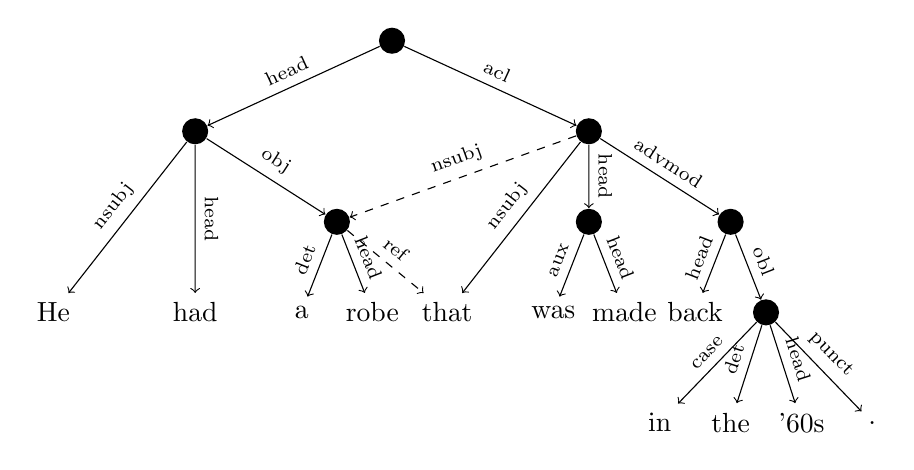
\begin{tikzpicture}[->,level distance=11.5mm,
	  level 1/.style={sibling distance=5cm},
	  level 2/.style={sibling distance=18mm},
	  level 3/.style={sibling distance=9mm},
	  level 4/.style={sibling distance=9mm,level distance=14mm},
	  every circle node/.append style={fill=black}]
	  \tikzstyle{word} = [font=\rmfamily,color=black]
	  \node (1_1) [circle] {}
	  {
	  child {node (1_2) [circle] {}
	    {
	    child {node {}
	    {
    	    child {node (1_6) [word] {He}  edge from parent [draw=none]}
    	} edge from parent [draw=none]}
	    child {node {}
	    {
    	    child {node (1_3) [word] {had}  edge from parent [draw=none]}
    	} edge from parent [draw=none]}
	    child {node (1_7) [circle] {}
	      {
	      child {node (1_14) [word] {a}  edge from parent node[midway,above,sloped]  {\scriptsize det}}
	      child {node (1_8) [word] {robe}  edge from parent node[midway,above,sloped]  {\scriptsize head}}
	      } edge from parent node[midway,above,sloped]  {\scriptsize obj}}
	    } edge from parent node[midway,above,sloped]  {\scriptsize head}}
	  child {node (1_4) [circle] {}
	    {
	    child {node {}
	    {
    	    child {node (1_15) [word] {that}  edge from parent [draw=none]}
    	} edge from parent [draw=none]}
	    child {node (1_5) [circle] {}
	      {
	      child {node (1_9) [word] {was}  edge from parent node[midway,above,sloped]  {\scriptsize aux}}
	      child {node (1_10) [word] {made}  edge from parent node[midway,above,sloped]  {\scriptsize head}}
	      } edge from parent node[midway,above,sloped]  {\scriptsize head}}
	    child {node (1_11) [circle] {}
	      {
	      child {node (1_12) [word] {back}  edge from parent node[midway,above,sloped]  {\scriptsize head}}
	      child {node (1_16) [circle] {}
	        {
	        child {node (1_18) [word] {in}  edge from parent node[midway,above,sloped]  {\scriptsize case}}
	        child {node (1_19) [word] {the}  edge from parent node[midway,above,sloped]  {\scriptsize det}}
	        child {node (1_17) [word] {'60s}  edge from parent node[midway,above,sloped]  {\scriptsize head}}
	        child {node (1_20) [word] {.}  edge from parent node[midway,above,sloped]  {\scriptsize punct}}
	        } edge from parent node[midway,above,sloped]  {\scriptsize obl}}
	      } edge from parent node[midway,above,sloped]  {\scriptsize advmod}}
	    } edge from parent node[midway,above,sloped]  {\scriptsize acl}}
	  };
	  \draw[->] (1_2) to node [midway,above,sloped] {\scriptsize nsubj} (1_6);
	  \draw[->] (1_2) to node [midway,above,sloped] {\scriptsize head} (1_3);
	  \draw[->] (1_4) to node [midway,above,sloped] {\scriptsize nsubj} (1_15);
	  \draw[dashed,->] (1_4) to node [midway,above,sloped] {\scriptsize nsubj} (1_7);
	  \draw[dashed,->] (1_7) to node [midway,above,sloped] {\scriptsize ref} (1_15);
	\end{tikzpicture}}
  \captionof{figure}{UD converted to unified DAG format.}\label{fig:converted_example_relcl}
\end{subfigure}}
\cprotect\caption{(a) \verb|reviews-255261-0007| (\verb|UD_English-EWT|), containing a relative clause,
and (b) the same graph after conversion to the unified DAG format.
The cycle is removed due to the non-terminal nodes introduced in the conversion.}
\label{fig:example_relcl}
\end{figure*}


\section{Unified DAG Format}\label{sec:format}

To apply TUPA to UD parsing,
we convert UD trees and graphs into a unified DAG format \cite{hershcovich2018multitask}.
The format consists of a rooted DAG, where the tokens are the terminal
nodes.\footnote{Our conversion code supports full conversion between UCCA and UD,
among other representation schemes,
and is publicly available at \url{http://github.com/danielhers/semstr/tree/master/semstr/conversion}.}
Edges are labeled (but not nodes),
and are divided into \textit{primary} and \textit{remote} edges,
where the primary edges form a tree (all nodes have at most one primary parent,
and the root has none).
Remote edges (denoted as dashed edges in Figure~\ref{fig:converted_examples})
enable reentrancy, and thus form a DAG together with primary edges.
Figure~\ref{fig:converted_examples} shows an example UCCA graph,
and a UD graph (containing two enhanced dependencies) before and after conversion.
Both annotate the same sentence from the
English Web Treebank \cite{L14-1067}\footnote{\url{https://catalog.ldc.upenn.edu/LDC2012T13}}.

\paragraph{Conversion protocol.}

To convert UD into the unified DAG format,
we add a pre-terminal for each token,
and attach the pre-terminals according to the original dependency edges:
traversing the tree from the root down, for each head token we create a non-terminal
parent with the edge label {\it head},
and add the node's dependents as children of the created non-terminal node
(see Figure~\ref{fig:converted_example_ud}).
This creates a constituency-like structure,
which is supported by TUPA's transition set (see \S\ref{sec:transition_setb}).

Although the enhanced dependency graph is not necessarily a supergraph
of the basic dependency tree,
the graph we convert to the unified DAG format is their union:
any enhanced dependnecies that are distinct from the basic dependency of a
node (by having a different head or universal dependency relation)
are converted to \textit{remote edges} in the unified DAG format.

To convert graphs in the unified DAG format back into dependency graphs,
we collapse all \textit{head} edges,
determining for each terminal what is the highest non-terminal headed by it,
and then attaching the terminals to each other according to the edges among
their headed non-terminals.

\paragraph{Input format.}

Enhanced dependencies are encoded in the 9th column of the \mbox{CoNLL-U} format,
by an additional head index, followed by a colon and dependency relation.
Multiple enhanced dependencies for the same node are separated by pipes.
Figure~\ref{fig:enhanced_conllu} demonstrates this format.
Note that if the basic dependency is repeated in the enhanced graph
(\verb|3:nsubj:pass| in the example), we do not treat it as an enhanced 
dependency, so that the converted graph will only contain each edge once.
In addition to the UD relations defined in the basic
representations, enhanced dependencies may contain the relation \verb|ref|,
used for relative clauses.
In addition, they may contain more specific relation subtypes,
and optionally also case information.

\paragraph{Language-specific extensions and case information.}

Dependencies may contain language-specific relation subtypes,
encoded as a suffix separated from the universal relation by a colon.
These extensions are ignored by the parsing evaluation metrics,
so for example, the subtyped relation \verb|nsubj:pass| (Figure~\ref{fig:original_examples})
is considered the same as the universal relation \verb|nsubj|
for evaluation purposes.
In the enhanced dependencies,
these suffixes may also contain case information,
which may be represented by the lemma of an adposition.
For example, the ``peace''~$\to$~``earth'' dependency in Figure~\ref{fig:example_ellipsis}
is augmented as \verb|nmod:on| in the enhanced graph
(not shown in the figure because it shares the universal relation with the basic dependency).

In the conversion process, we strip any language-specific extensions
from both basic and enhanced dependencies,
leaving only the universal relations.
Consequently, case information that might be encoded in the enhanced
dependencies is lost, and we do not handle it in our current system.

\paragraph{Ellipsis and null nodes.}

In addition to enhanced dependencies, the enhanced UD representation
adds null nodes to represented elided predicates.
These, too, are ignored in the standard evaluation.
An example is shown in Figure~\ref{fig:example_ellipsis},
where an elided ``wish'' is represented by the node E9.1.
The elided predicate's dependents are attached to its argument ``peace''
in the basic representation, and the argument itself is attached as an \verb|orphan|.
In the enhanced representation, all arguments are attached to the null node as if
the elided predicate was present.

While UCCA supports empty nodes without surface realization
in the form of \textit{implicit units},
previous work on UCCA parsing has removed these from the graphs.
We do the same for UD parsing, dropping null nodes and their
associated dependencies upon conversion to the unified DAG format.
We leave parsing elided predicates for future work.

\paragraph{Propagation of conjuncts.}

Enhanced dependencies contain dependencies between conjoined predicates
and their arguments, and between predicates and their conjoined arguments
or modifiers.
While these relations can often be inferred from the basic dependencies,
in many cases they require semantic knowledge to parse correctly.
For example, in Figure~\ref{fig:example_conj},
the enhanced dependencies represent the shared subject (``he'') among the
conjoined predicates (``went'' and ``finished''),
and the conjoined modifiers (``efficiently'' and ``promptly'')
for the second predicate (``finished'').
However, there are no enhanced dependencies between the first predicate
and the second predicate's modifiers (e.g. ``went''~$\to$~``efficiently''),
as semantically only the subject is shared and not the modifiers.

\paragraph{Relative clauses.}

Finally, enhanced graphs attach predicates of relative clauses directly
to the antecedent modified by the relative clause, adding a \verb|ref|
dependency between the antecedent and the relative pronoun.
An example is shown in Figure~\ref{fig:example_relcl_ud}.
While these graphs may contain cycles
(``robe''~$\leftrightarrow$~``made''
in the example), they are removed upon conversion to
the unified DAG format by the introduction of non-terminal nodes
(see Figure~\ref{fig:converted_example_relcl}).


%%%%%%%%%%%%%%%%%%%%%%%%%%%%%%%%%%%%%%%%%%%%%%%%%%%%%%%%%%%%%%%
\section{General Transition-based DAG Parser}\label{sec:model}

We now turn to describing TUPA \cite{hershcovich2017a,hershcovich2018multitask},
a general transition-based parser \cite{Nivre03anefficient}.
TUPA uses an extended set of transitions and features that supports
reentrancies, discontinuities and non-terminal nodes.
The parser state is composed of a buffer $B$ of tokens and nodes to be processed,
a stack $S$ of nodes currently being processed,
and a graph $G=(V,E,\ell)$ of constructed nodes and edges,
where $V$ is the set of \emph{nodes}, $E$ is the set of \emph{edges},
and $\ell : E \to L$ is the \emph{label} function, $L$ being the set of possible labels.
Some states are marked as \textit{terminal}, meaning that $G$ is the final output.
A classifier is used at each step to select the next transition based on features
encoding the parser's current state.
During training, an oracle creates training instances for the classifier,
based on gold-standard annotations.

\begin{figure*}
	\begin{adjustbox}{width=\textwidth,margin=3pt,frame}
	\begin{tabular}{llll|l|llllc|c}
		\multicolumn{4}{c|}{\textbf{\small Before Transition}} & \textbf{\small Transition} & \multicolumn{5}{c|}{\textbf{\small After Transition}} & \textbf{\small Condition} \\
		\textbf{\footnotesize Stack} & \textbf{\footnotesize Buffer} & \textbf{\footnotesize Nodes} & \textbf{\footnotesize Edges} & & \textbf{\footnotesize Stack} & \textbf{\footnotesize Buffer} & \textbf{\footnotesize Nodes} & \textbf{\footnotesize Edges} & \textbf{\footnotesize Terminal?} & \\
		$S$ & $x \;|\; B$ & $V$ & $E$ & \textsc{Shift} & $S \;|\; x$ & $B$ & $V$ & $E$ & $-$ & \\
		$S \;|\; x$ & $B$ & $V$ & $E$ & \textsc{Reduce} & $S$ & $B$ & $V$ & $E$ & $-$ & \\
		$S \;|\; x$ & $B$ & $V$ & $E$ & \textsc{Node$_X$} & $S \;|\; x$ & $y \;|\; B$ & $V \cup \{ y \}$ & $E \cup \{ (y,x)_X \}$ & $-$ &
		$x \neq \mathrm{root}$ \\
		$S \;|\; y,x$ & $B$ & $V$ & $E$ & \textsc{Left-Edge$_X$} & $S \;|\; y,x$ & $B$ & $V$ & $E \cup \{ (x,y)_X \}$ & $-$ &
		\multirow{4}{50pt}{\vspace{-5mm}\[\left\{\begin{array}{l}
		x \not\in w_{1:n},\\
		y \neq \mathrm{root},\\
		y \not\leadsto_G x
		\end{array}\right.\]} \\
		$S \;|\; x,y$ & $B$ & $V$ & $E$ & \textsc{Right-Edge$_X$} & $S \;|\; x,y$ & $B$ & $V$ & $E \cup \{ (x,y)_X \}$ & $-$ & \\
		$S \;|\; y,x$ & $B$ & $V$ & $E$ & \textsc{Left-Remote$_X$} & $S \;|\; y,x$ & $B$ & $V$ & $E \cup \{ (x,y)_X^* \}$ & $-$ & \\
		$S \;|\; x,y$ & $B$ & $V$ & $E$ & \textsc{Right-Remote$_X$} & $S \;|\; x,y$ & $B$ & $V$ & $E \cup \{ (x,y)_X^* \}$ & $-$ & \\
		$S \;|\; x,y$ & $B$ & $V$ & $E$ & \textsc{Swap} & $S \;|\; y$ & $x \;|\; B$ & $V$ & $E$ & $-$ &
		$\mathrm{i}(x) < \mathrm{i}(y)$ \\
		$[\mathrm{root}]$ & $\emptyset$ & $V$ & $E$ & \textsc{Finish} & $\emptyset$ & $\emptyset$ & $V$ & $E$ & $+$ & \\
	\end{tabular}
	\end{adjustbox}
	\caption{\label{fig:transitionsb}
	  The transition set of TUPA.
	  We write the stack with its top to the right and the buffer with its head to the left.
	  $(\cdot,\cdot)_X$ denotes a primary $X$-labeled edge, and $(\cdot,\cdot)_X^*$ a remote $X$-labeled edge.
	  $\mathrm{i}(x)$ is the swap index (see \S\ref{sec:constraints}).
	  In addition to the specified conditions,
	  the prospective child in an \textsc{Edge} transition must not already have a primary parent.
	}
\end{figure*}

\subsection{Transition Set}\label{sec:transition_setb}
Given a sequence of tokens $w_1, \ldots, w_n$,
we predict a rooted graph $G$ whose terminals are the tokens.
Parsing starts with the root node on the stack,
and the input tokens in the buffer.

The TUPA transition set, shown in Figure~\ref{fig:transitionsb}, includes
the standard \textsc{Shift} and \textsc{Reduce} operations,
\textsc{Node$_X$} for creating a new non-terminal node and an $X$-labeled edge,
\textsc{Left-Edge$_X$} and \textsc{Right-Edge$_X$} to create a new primary $X$-labeled edge,
\textsc{Left-Remote$_X$} and \textsc{Right-Remote$_X$} to create a new remote $X$-labeled edge,
\textsc{Swap} to handle discontinuous nodes,
and \textsc{Finish} to mark the state as terminal.

The \textsc{Remote$_X$} transitions are not required for parsing trees,
but as we treat the problem as general DAG parsing due to the inclusion of enhanced dependencies,
we include these transitions.


\begin{figure}[t]\centering
   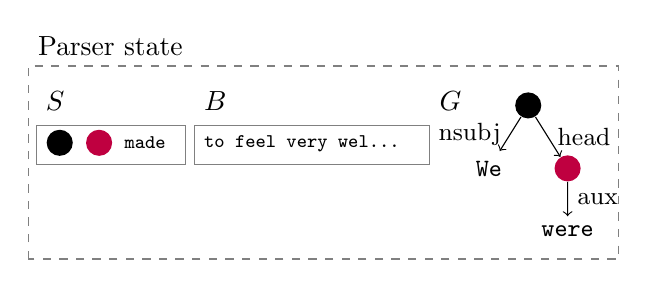
\begin{tikzpicture}[level distance=8mm, sibling distance=1cm]
   \node[anchor=west] at (0,1.5) {Parser state};
   \draw[color=gray,dashed] (0,-1.2) rectangle (7.5,1.25);
   \draw[color=gray] (.1,0) rectangle (2,.5);
   \node[anchor=west] at (.1,.8) {$S$};
   \node[fill=black, circle] at (.4,.275) {};
   \node[fill=purple, circle] at (.9,.275) {};
   \node[anchor=west] at (1.1,.275) {\scriptsize\ttfamily made};
   \draw[color=gray] (2.11,0) rectangle (5.1,.5);
   \node[anchor=west] at (2.11,.8) {$B$};
   \node[anchor=west] at (2.11,.26) {\scriptsize\ttfamily to feel very wel\ldots};
   \node[anchor=west] at (5.1,.8) {$G$};
   \node[fill=black, circle] at (6.35,.75) {}   
     child {node  {\small\ttfamily We} edge from parent [->] node[left] {\small nsubj}}
     child {node [fill=purple, circle] {}
     {
       child {node {\small\ttfamily were} edge from parent [->] node[right] {\small aux}}
     } edge from parent [->] node[right] {\small head} };
   \end{tikzpicture}
   
   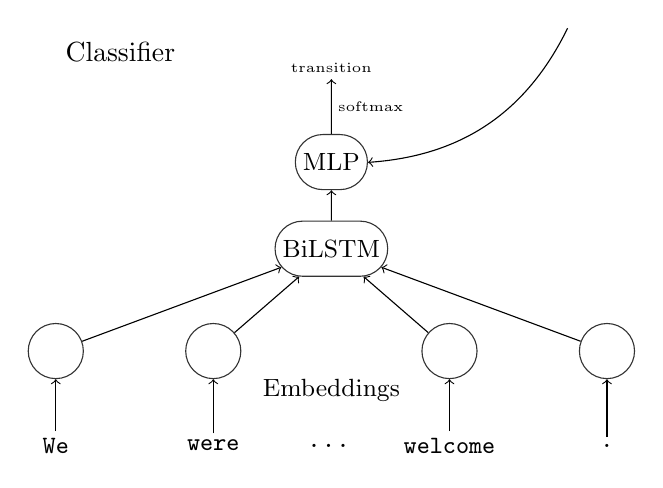
\begin{tikzpicture}[->]
   \node[anchor=west] at (0,6) {Classifier};
   \tiny
   \tikzstyle{main}=[rounded rectangle, minimum size=7mm, draw=black!80, node distance=12mm]
   \node[main] (specific) at (3.5,3.5) {\small BiLSTM};
   \node (embeddings) at (3.5,1.7) {\small Embeddings};
   \foreach \i/\word in {0/{We},2/{were},5/{welcome},7/{.}} {
       \node (x\i) at (\i,1) {\small\ttfamily\word};
       \node[main] (e\i) at (\i,2.2) {};
       \path (x\i) edge (e\i);
       \path (e\i) edge (specific);
   }
    \node (x4) at (3.5,1) {\large\ldots};
    \node[main] (mlp) at (3.5,4.6) {\small MLP};
    \path (specific) edge (mlp);
    \coordinate (state) at (6.5,6.3);
    \path (state) edge [bend left] (mlp);
    \node (transition) at (3.5,5.8) {transition};
    \path (mlp) edge node[right] {softmax} (transition);
   \end{tikzpicture}
\caption{Illustration of the TUPA model, adapted from \citet{hershcovich2018multitask}.
Top: parser state (stack, buffer and intermediate graph).
		Bottom: BiLTSM architecture.
		Vector representation for the input tokens is computed
		by two layers of bidirectional LSTMs.
		The vectors for specific tokens are concatenated with
		embedding and numeric features from the parser state
		(for existing edge labels, number of children, etc.),
		and fed into the MLP for selecting the next transition.}\label{fig:single_modela}
\end{figure}


%%%%%%%%%%%%%%%%%%%%%%%%%%%%%%%%%%%%%%%%%%%%%%%%%%%%%%%%%%%%%%%%%%%%%%%%%%%%%%%%%
\subsection{Transition Classifier}\label{sec:classifierc}

To predict the next transition at each step,
TUPA uses a BiLSTM with feature embeddings as inputs,
followed by an MLP and a softmax layer for classification.
The model is illustrated in Figure~\ref{fig:single_modela}.
Inference is performed greedily,
and training is done with an oracle that yields the set of all optimal 
transitions at a given state (those that lead to a state from which the gold graph is still reachable).
Out of this set, the actual transition performed in training is the one
with the highest score given by the classifier,
which is trained to maximize the sum of log-likelihoods of all 
optimal transitions at each step.




\paragraph{Features.}

We use vector embeddings
representing the words, lemmas, coarse (universal) POS tags and fine-grained POS tags,
provided by UDPipe 1.2 during test.
For training, we use the gold-annotated lemmas and POS tags.
In addition, we use one-character prefix, three-character suffix,
shape (capturing orthographic features, e.g., ``Xxxx'') and named entity type,
provided by spaCy;\footnote{\url{http://spacy.io}}
punctuation and gap type features \cite{maier-lichte:2016:DiscoNLP},
and previously predicted edge labels and parser actions.
These embeddings are initialized randomly, except for the word embeddings,
which are initialized with the 250K most frequent word vectors from fastText
for each language
\cite{bojanowski2016enriching},\footnote{\url{http://fasttext.cc}}
pre-trained over Wikipedia and updated during training.
We do not use word embeddings for languages without pre-trained fastText vectors
(Ancient Greek, North Sami and Old French).

To the feature embeddings, we concatenate
numeric features representing the node height, number of (remote) parents and children,
and the ratio between the number of terminals to total number of nodes in the graph $G$.

Table~\ref{tab:featuresc} lists all feature used for the classifier.
Numeric features are taken as they are, whereas categorical features are mapped to real-valued embedding
vectors.
For each non-terminal node,
we select a \textit{head terminal} for feature extraction,
by traversing down the graph according to
a priority order on edge labels (otherwise selecting the leftmost child).
The priority order is:
\begin{verbatim}
parataxis, conj, advcl, xcomp
\end{verbatim}


\begin{table}[ht]
\centering
\small
\begin{tabular}{l|l}
\hline
\bf Nodes & \\
$s_0$ & \texttt{wmtuepT\#\^{}\$xhqyPCIEMN} \\
$s_1$ & \texttt{wmtueT\#\^{}\$xhyN} \\
$s_2$ & \texttt{wmtueT\#\^{}\$xhy} \\
$s_3$ & \texttt{wmtueT\#\^{}\$xhyN} \\
$b_0$ & \texttt{wmtuT\#\^{}\$hPCIEMN} \\
$b_1, b_2, b_3$ & \texttt{wmtuT\#\^{}\$} \\
\multirow{3}{90pt}{$s_0l, s_0r, s_1l, s_1r,$ $s_0ll, s_0lr,s_0rl, s_0rr,$ $s_1ll, s_1lr, s_1rl, s_1rr$} &
    \texttt{wme\#\^{}\$} \\\\\\
\multirow{2}{90pt}{$s_0L, s_0R, s_1L,$ $s_1R, b_0L, b_0R$} & \texttt{wme\#\^{}\$} \\\\
\hline
\bf Edges & \\
\multirow{2}{90pt}{$s_0 \to s_1, s_0 \to b_0,$ $s_1 \to s_0, b_0 \to s_0$} & \texttt{x} \\\\
$s_0 \to b_0, b_0 \to s_0$ & \texttt{e} \\
\hline
\bf Past actions \\
$a_0, a_1$ & \texttt{eA} \\
\hline
\bf Global & \texttt{node ratio}
\end{tabular}
\caption{Transition classifier features.\label{tab:featuresc}\\
$s_i$: stack node $i$ from the top.
$b_i$: buffer node $i$.\\
$xl$, $xr$ ($xL$, $xR$): $x$'s leftmost and rightmost children (parents).
\texttt{w}: head terminal text.
\texttt{m}: lemma.
\texttt{u}: coarse (universal) POS tag.
\texttt{t}: fine-grained POS tag.
\texttt{h}: node's height.
\texttt{e}: label of its first incoming edge.
\texttt{p}: any separator punctuation between $s_0$ and $s_1$.
\texttt{q}: count of any separator punctuation between $s_0$ and $s_1$.
\texttt{x}: numeric value of gap type \cite{maier-lichte:2016:DiscoNLP}.
\texttt{y}: sum of gap lengths.
\texttt{P}, \texttt{C}, \texttt{I}, \texttt{E}, and \texttt{M}: number of
parents, children, implicit children, remote children, and remote parents.
\texttt{N}: numeric value of the head terminal's named entity IOB indicator.
\texttt{T}: named entity type.
\texttt{\#}: word shape (capturing orthographic features, e.g. "Xxxx" or "dd").
\texttt{\^{}}: one-character prefix.
\texttt{\$}: three-character suffix.\\
$x \to y$ refers to the existing edge from $x$ to $y$.
\texttt{x} is an indicator feature, taking the value of 1 if the edge exists or 0 otherwise,
\texttt{e} refers to the edge label, and
$a_i$ to the transition taken $i+1$ steps ago.\\
\texttt{A} refers to the action type (e.g. \textsc{shift}/\textsc{right-edge}/\textsc{node}), and
\texttt{e} to the edge label created by the action.\\
\texttt{node ratio} is the ratio between non-terminals and terminals \cite{hershcovich2017a}.}
\end{table}

\subsection{Constraints}\label{sec:constraints}
During training and parsing, we apply constraints on the parser state
to limit the possible transitions to valid ones.

A generic constraint implemented in TUPA is that stack nodes 
that have been swapped
should not be swapped again \cite{hershcovich2018multitask}.
 To implement this constraint, we define a \textit{swap index}
 for each node, assigned when the node is created.
 At initialization, only the root node and terminals exist.
 We assign the root a swap index of 0, and for each terminal, its
 position in the text (starting at 1).
 Whenever a node is created as a result of a \textsc{Node}
 transition, its swap index is the arithmetic
 mean of the swap indices of the stack top and buffer head.
 
In addition, we enforce UD-specific constraints, resulting from
the nature of the converted DAG format:
every non-terminal node must have a single outgoing \verb|head| edge:
once it has one, it may not get another, and
until it does, the node may not be reduced.


\section{Training details}\label{sec:details}

The model is implemented using DyNet v2.0.3
\cite{neubig2017dynet}.\footnote{\url{http://dynet.io}}
Unless otherwise noted, we use the default values provided by the package.
We use the same hyperparameters as used in previous experiments on UCCA
parsing \cite{hershcovich2018multitask},
without any hyperparameter tuning on UD treebanks.


\begin{table}[ht]
\centering
\begin{tabular}{l|c|ccccc}
\hline
\bf Hyperparameter &  \bf Value \\
\hline
Pre-trained word dim. & 300 \\
Lemma dim. & 200 \\
Coarse (universal) POS tag dim. & 20 \\
Fine-grained POS tag dim. & 20 \\
Named entity dim. & 3 \\
Punctuation dim. & 1 \\
Shape dim. & 3 \\
Prefix dim. & 2 \\
Suffix dim. & 3 \\
Action dim. & 3 \\
Edge label dim. & 20 \\
\hline
MLP layers & 2 \\
MLP dimensions & 50 \\
BiLSTM layers & 2 & \\
BiLSTM dimensions & 500
\end{tabular}
\caption{Hyperparameter settings.\label{tab:hyperparamsc}}
\end{table}


\subsection{Hyperparameters}

We use dropout \cite{srivastava2014dropout} between MLP layers, and recurrent dropout
\cite{NIPS2016_6241} between BiLSTM layers, both with $p=0.4$.
We also use word, lemma, coarse- and fine-grained POS tag dropout
with $\alpha=0.2$
\cite{kiperwasser2016simple}: in training, the embedding for a feature value
$w$ is replaced with a zero vector with a probability of
$\frac{\alpha}{\#(w)+\alpha}$,
where $\#(w)$ is the number of occurrences of $w$ observed.
In addition, we use \textit{node dropout} \cite{hershcovich2018multitask}:
with a probability of 0.1 at each step, all features associated with a single
node in the parser state are replaced with zero vectors.
For optimization we use a minibatch size of 100, decaying all weights by $10^{-5}$ at each update,
and train with stochastic gradient descent for $50$ epochs with a learning
rate of 0.1, followed by AMSGrad \cite{j.2018on} for $250$ epochs with
$\alpha=0.001,\beta_1=0.9$ and $\beta_2=0.999$.
We found this training strategy better than using only one of the optimization methods,
similar to findings by \citet{keskar2017improving}.
We select the epoch with the best LAS-F1 on the
development set.
Other hyperparameter settings are listed in Table~\ref{tab:hyperparamsc}.

\subsection{Small Treebanks}

For corpora with less than 100 training sentences,
we use $750$ epochs of AMSGrad instead of $250$.
For corpora with no development set,
we use 10-fold cross-validation on the training set,
each time splitting it to 80\% training, 10\% development and 10\% validation.
We perform the normal training procedure on the training and development
subsets, and then select the model from the fold with the best LAS-F1
on the corresponding validation set.

\subsection{Multilingual Model}

For the purpose of parsing languages with no training data,
we use a delexicalized multilingual model, trained on the shuffled training sets
from all corpora, with no word, lemma, fine-grained tag, prefix and suffix features.
We train this model for two epochs using stochastic gradient descent
with a learning rate of $0.1$
(we only trained this many epochs due to time constraints).

\subsection{Out-of-domain Evaluation}

For test treebanks without corresponding training data,
but with training data in the same language, during testing
we use the model trained on the largest training treebank in the same language.


\section{Results}\label{sec:resultsc}

Official evaluation was done on the TIRA online platform \cite{tira}.
Our system (named ``HUJI'') ranked 24th in the LAS-F1 ranking
(with an average of 53.69 over all test treebanks),
23rd by MLAS (average of 44.6) and 21st by BLEX (average of 48.05).
Since our system only performs dependency parsing and not other pipeline tasks,
we henceforth focus on LAS-F1 \cite{nivre17udw} for evaluation.

After the official evaluation period ended,
we discovered several bugs in the conversion between the CoNLL-U format
and the unified DAG format, which is used by TUPA for training and is output by it
(see~\S\ref{sec:format}).
We did not re-train TUPA on the training treebanks after fixing these bugs,
but we did re-evaluate the already trained models on all test treebanks,
and used the fixed code for converting their output to CoNLL-U.
This yielded an unofficial average test LAS-F1 of 58.48,
an improvement of 4.79 points over the official average score.
In particular, for two test sets, \verb|ar_padt| and \verb|gl_ctg|, TUPA got
a zero score in the official evaluation due to a bug with the treatment of multi-token words.
These went up to 61.9 and 71.42, respectively.
We also evaluated the trained TUPA models on all available development treebanks
after fixing the bugs.

Table~\ref{tab:overall_results} presents the
averaged scores on the shared task test sets,
and Figure~\ref{fig:test_per_corpus} the (official and unofficial) LAS-F1
scores obtained by TUPA on each of the test and development treebanks.

\begin{table}
\begin{tabular}{lccc}
\hline
& \multirow{2}{32mm}{\bf TUPA {\small(official)}} & \multirow{2}{35mm}{\bf TUPA {\small(unofficial)}}
& \multirow{2}{34mm}{\bf UDPipe {\small(baseline)}} \\\\
\hline
All treebanks & 53.69 & 58.48 & 65.80 \\
Big treebanks & 62.07 & 67.36 & 74.14 \\
PUD treebanks & 56.35 & 56.82 & 66.63 \\
Small treebanks & 36.74 & 41.19 & 55.01 \\
Low-resource & 8.53 & 12.68 & 17.17
\end{tabular}
\caption{Aggregated test LAS-F1 scores
for our system (TUPA) and the baseline system (UDPipe 1.2).
\label{tab:overall_results}}
\end{table}

\catcode`\_=12
\pgfplotstableread{
corpus
af_afribooms
grc_perseus
grc_proiel
ar_padt
hy_armtdp
eu_bdt
br_keb
bg_btb
bxr_bdt
ca_ancora
hr_set
cs_cac
cs_fictree
cs_pdt
cs_pud
da_ddt
nl_alpino
nl_lassysmall
en_ewt
en_gum
en_lines
en_pud
et_edt
fo_oft
fi_ftb
fi_pud
fi_tdt
fr_gsd
}\corpusa
\pgfplotstableread{
corpus
fr_sequoia
fr_spoken
gl_ctg
gl_treegal
de_gsd
got_proiel
el_gdt
he_htb
hi_hdtb
hu_szeged
zh_gsd
id_gsd
ga_idt
it_isdt
it_postwita
ja_gsd
ja_modern
kk_ktb
ko_gsd
ko_kaist
kmr_mg
la_ittb
la_perseus
la_proiel
lv_lvtb
pcm_nsc
sme_giella
}\corpusb
\pgfplotstableread{
corpus
no_bokmaal
no_nynorsk
no_nynorsklia
fro_srcmf
cu_proiel
fa_seraji
pl_lfg
pl_sz
pt_bosque
ro_rrt
ru_syntagrus
ru_taiga
sr_set
sk_snk
sl_ssj
sl_sst
es_ancora
sv_lines
sv_pud
sv_talbanken
th_pud
tr_imst
uk_iu
hsb_ufal
ur_udtb
ug_udt
vi_vtb
}\corpusc

\begin{figure*}[h!]
    \begin{tikzpicture}
    \begin{axis}[
    ybar=0pt,  
    enlarge x limits={0.02},
    enlarge y limits={value=0.3,upper},
    ymin=0,
    width=18cm,
    height=8cm,
    bar width=4pt,
    xtick=data,
    xticklabels from table={\corpusa}{corpus},
    xticklabel style={font=\tiny,rotate=75,anchor=east},
    xtick align=inside,
    xticklabel pos=left,
    yticklabels=none,
    tickwidth=0pt,
    legend style={at={(axis cs:0,113)},anchor=north west},
    legend cell align={left},
    nodes near coords={
     \scalebox{.4}{\pgfmathprintnumber[precision=2]{\pgfplotspointmeta}}
    },
    every node near coord/.append style={rotate=90,anchor=west}
    ]
    \addplot[select coords between index={0}{27},fill=green]table[x expr=\coordindex,meta=corpus,y=official]{udst2018scores.txt};
    \addplot[select coords between index={0}{27},fill=red]table[x expr=\coordindex,meta=corpus,y=test]{udst2018scores.txt};
    \addplot[select coords between index={0}{27},fill=blue]table[x expr=\coordindex,meta=corpus,y=dev]{udst2018scores.txt};
    \legend{Test (official), Test (unofficial), Development}
    \end{axis}
    \end{tikzpicture}
   
    \begin{tikzpicture}
    \begin{axis}[
    ybar=0pt,  
    enlarge x limits={0.02},
    enlarge y limits={value=0.15,upper},
    ymin=0,
    width=18cm,
    height=8cm,
    bar width=4pt,
    xtick=data,
    xticklabels from table={\corpusb}{corpus},
    xticklabel style={font=\tiny,rotate=75,anchor=east},
    xtick align=inside,
    xticklabel pos=left,
    yticklabels=none,
    tickwidth=0pt,
    nodes near coords={
     \scalebox{.4}{\pgfmathprintnumber[precision=2]{\pgfplotspointmeta}}
    },
    every node near coord/.append style={rotate=90, anchor=west}
    ]
    \addplot[select coords between index={28}{54},fill=green]table[x expr=\coordindex,meta=corpus,y=official]{udst2018scores.txt};
    \addplot[select coords between index={28}{54},fill=red]table[x expr=\coordindex,meta=corpus,y=test]{udst2018scores.txt};
    \addplot[select coords between index={28}{54},fill=blue]table[x expr=\coordindex,meta=corpus,y=dev]{udst2018scores.txt};
    \end{axis}
    \end{tikzpicture}
   
    \begin{tikzpicture}
    \begin{axis}[
    ybar=0pt,  
    enlarge x limits={0.02},
    enlarge y limits={value=0.15,upper},
    ymin=0,
    width=18cm,
    height=8cm,
    bar width=4pt,
    xtick=data,
    xticklabels from table={\corpusc}{corpus},
    xticklabel style={font=\tiny,rotate=75,anchor=east},
    xtick align=inside,
    xticklabel pos=left,
    yticklabels=none,
    tickwidth=0pt,
    nodes near coords={
     \scalebox{.4}{\pgfmathprintnumber[precision=2]{\pgfplotspointmeta}}
    },
    every node near coord/.append style={rotate=90, anchor=west}
    ]
    \addplot[select coords between index={55}{81},fill=green]table[x expr=\coordindex,meta=corpus,y=official]{udst2018scores.txt};
    \addplot[select coords between index={55}{81},fill=red]table[x expr=\coordindex,meta=corpus,y=test]{udst2018scores.txt};
    \addplot[select coords between index={55}{81},fill=blue]table[x expr=\coordindex,meta=corpus,y=dev]{udst2018scores.txt};
    \end{axis}
    \end{tikzpicture}
    \caption{TUPA's LAS-F1 per treebank: official and unofficial test scores, and development scores (where available).
    \label{fig:test_per_corpus}}
\end{figure*}
\catcode`\_=8


\subsection{Evaluation on Enhanced Dependencies}\label{sec:enhanced_results}

Since the official evaluation ignores enhanced dependencies,
we evaluate them separately using a modified version of the shared task evaluation
script\footnote{\url{https://github.com/CoNLL-UD-2018/HUJI/blob/master/tupa/scripts/conll18_ud_eval.py}}.
We calculate the \textit{enhanced LAS},
identical to the standard LAS except that the set of dependencies
in both gold and predicted graphs are the enhanced dependencies instead
of the basic dependencies:
ignoring null nodes and any enhanced dependency sharing a head with a basic one,
we align the words in the gold graph and the system's graph as in the standard LAS,
and define
\[
P=\frac{\#\mathrm{correct}}{\#\mathrm{system}},
R=\frac{\#\mathrm{correct}}{\#\mathrm{gold}},
F1=2\cdot\frac{P\cdot R}{P+R}.
\]

Table~\ref{tab:enhanced} lists the enhanced LAS precision, recall and F1 score
on the test treebanks with any enhanced dependencies,
as well as the percentage of enhanced dependencies in each test treebank,
calculated as
$100 \cdot \frac{\#\mathrm{enhanced}}{\#\mathrm{enhanced} + \#\mathrm{words}}$.

Just as remote edges in UCCA parsing are more challenging
than primary edges \cite{hershcovich2017a},
parsing enhanced dependencies is a harder task than standard UD parsing,
as the scores demonstrate.
However, TUPA learns them successfully, getting as much as 56.55 enhanced LAS-F1
(on the Polish LFG test set).

\catcode`\_=12
\begin{table}[t]
\begin{tabular}{l|ccc|c}
\hline
& \multicolumn{3}{c|}{Enhanced LAS} & \multirow{2}{11mm}{\% Enhanced} \\
\bf Treebank & \bf P & \bf R & \bf F1 & \\
\hline
ar_padt & 28.51 & 16.24 & 20.69 & 5.30\\ 
cs_cac & 54.94 & 35.69 & 43.27 & 7.57\\ 
cs_fictree & 48.78 & 18.53 & 26.85 & 4.30\\ 
cs_pdt & 49.46 & 26.47 & 34.48 & 4.61\\ 
nl_alpino & 56.04 & 50.81 & 53.30 & 4.80\\ 
nl_lassysmall & 49.71 & 51.30 & 50.49 & 4.13\\ 
en_ewt & 57.36 & 52.05 & 54.58 & 4.36\\ 
en_pud & 58.99 & 50.00 & 54.13 & 5.14\\ 
fi_tdt & 40.20 & 31.37 & 35.24 & 7.34\\ 
lv_lvtb & 31.76 & 18.70 & 23.54 & 4.12\\ 
pl_lfg & 59.19 & 54.13 & 56.55 & 2.61\\ 
sk_snk & 37.28 & 21.61 & 27.36 & 3.91\\ 
sv_pud & 45.40 & 39.58 & 42.29 & 6.36\\ 
sv_talbanken & 50.15 & 43.20 & 46.42 & 6.89
\end{tabular}
\caption{TUPA's enhanced LAS precision, recall and F1 per test treebank with 
any enhanced dependencies,
and percentage of enhanced dependencies in test treebank.
\label{tab:enhanced}}
\end{table}
\catcode`\_=8

\subsection{Ablation Experiments}\label{sec:ablation}

The TUPA transition classifier for some of the languages uses
named entity features calculated by
spaCy.\footnote{\url{https://spacy.io/api/annotation}}
For German, Spanish, Portuguese, French, Italian, Dutch and Russian,
the spaCy named entity recognizer was trained
on Wikipedia \cite{nothman2013learning}.
However, the English model was trained on
OntoNotes\footnote{\url{https://catalog.ldc.upenn.edu/LDC2013T19}},
which is in fact not among the additional resources allowed by the shared task
organizers.
To get a fair evaluation
and to quantify the contribution of the NER features,
we re-trained TUPA on the English EWT (\verb|en_ewt|) training set
with the same hyperparameters as in our submitted model,
just without these features.
As Table~\ref{tab:ablation} shows,
removing the NER features ($-$NER) only slightly hurts the performance,
by 0.28 LAS-F1 points on the test treebank,
and 0.63 on the development treebank. 

As further ablation experiments, we tried removing POS features,
pre-trained word embeddings,
and remote edges (the latter enabling TUPA to parse enhanced dependencies).
Removing the POS features does hurt performance to a larger degree,
by 2.87 LAS-F1 points on the test set,
while removing the pre-trained word embeddings
even slightly improves the performance.
Removing remote edges and transitions from TUPA causes a very small decrease
in LAS-F1, and of course enhanced dependencies can then no longer be produced at all.


\begin{table}[t]
\begin{tabular}{l|cc|cc}
\hline
& \multicolumn{2}{c|}{\small LAS-F1} & \multicolumn{2}{c}{\small Enhanced LAS-F1} \\
\bf Model & \bf Test & \bf Dev & \bf Test & \bf Dev \\
\hline
Original & 72.10 & 72.44 & 54.58 & 57.13 \\
%Re-trained & 72.07 & 72.08 & 54.71 & 55.97\\ 
$-$NER & 71.82 & 71.81 & 55.31 & 54.65\\ 
$-$POS & 69.23 & 69.54 & 53.78 & 49.12\\ 
$-$Embed. & 72.33 & 72.55 & 56.26 & 54.54\\ 
$-$Remote & 72.08 & 72.32 & 0.00 & 0.00\\ 
%$-$Remote$-$NER & 71.36 & 71.78 & 0.00 & 0.00\\ 
%$-$Remote$-$Embed. & 72.22 & 72.44 & 0.00 & 0.00
\end{tabular}
\caption{Ablation LAS-F1 and Enhanced LAS-F1 on the English EWT development
and test set.
NER: named entity features.
POS: part-of-speech tag features (both universal and fine-grained).
Embed.: external pre-trained word embeddings (fastText).
Remote: remote edges and transitions in TUPA.
\label{tab:ablation}}
\end{table}

\section{Conclusion}\label{sec:conclusionc}

We have presented the HUJI submission to the CoNLL 2018 shared task on parsing Universal Dependencies, based on TUPA, a general transition-based DAG parser.
Using a simple conversion protocol to convert UD into a unified DAG format,
training TUPA as-is on the UD treebanks yields results
close to the UDPipe baseline for most treebanks in the standard evaluation.
While other systems ignore enhanced dependencies,
TUPA learns to produce them too as part of the general dependency parsing process.
We believe that with hyperparameter tuning and more careful handling of
cross-lingual and cross-domain parsing, TUPA can be competitive on the standard metrics too.

Furthermore, the generic nature of our parser, which supports many representation schemes, as well as domains and languages,
will allow improving performance by multitask learning \citep[cf.][]{hershcovich2018multitask},
which we plan to explore in future work.


\section*{Acknowledgments}

This work was supported by the Israel Science Foundation (grant no. 929/17) and
by the HUJI Cyber Security Research Center
in conjunction with the Israel National Cyber Bureau in the Prime Minister's Office.

%
% File divergences.tex

\chapter{Content Differences in Syntactic and Semantic Representations (Published in NAACL-HLT 2019)}\label{divergences}


\subsubsection*{Daniel Hershcovich$^{1,2}$, Omri Abend$^2$ and Ari Rappoport$^2$ \\
  $^1$The Edmond and Lily Safra Center for Brain Sciences \\
  $^2$School of Computer Science and Engineering \\
  Hebrew University of Jerusalem \\
  \texttt{\{danielh,oabend,arir\}@cs.huji.ac.il}  
}

\section*{Abstract}
  Syntactic analysis plays an important role in semantic parsing,
  but the nature of this role remains a topic of ongoing debate.
  The debate has been constrained by the scarcity of empirical comparative studies between syntactic and semantic schemes,
  which hinders the development of parsing methods informed by the details of target schemes and constructions.
  We target this gap, and take Universal Dependencies (UD) and UCCA as a test case.
  After abstracting away from differences of convention or formalism,
  we find that most content divergences can be ascribed to: 
  (1) UCCA's distinction between a Scene and a non-Scene;
  (2) UCCA's distinction between primary relations, secondary ones and participants;
  (3) different treatment of multi-word expressions, and
  (4) different treatment of inter-clause linkage.
  We further discuss the long tail of cases where the two schemes take markedly
  different approaches.
  Finally, we show that the proposed comparison methodology can be used
  for fine-grained evaluation of UCCA parsing,
  highlighting both challenges and potential sources for improvement.
  The substantial differences between the schemes suggest that
  semantic parsers are likely to benefit downstream text understanding applications
  beyond their syntactic counterparts.


\section{Introduction}\label{sec:introductiond}
  
  Semantic representations hold promise due to
  their ability to transparently reflect distinctions relevant for text understanding
  applications. For example, syntactic representations
  are usually sensitive to distinctions based on POS (part of speech), such as between compounds
  and possessives. Semantic schemes are  less likely to make
  this distinction since a possessive can often be paraphrased as a compound
  and vice versa (e.g., ``US president''/``president of the US''),
  but may distinguish different senses of possessives (e.g., ``some of the presidents'' and ``inauguration of the presidents'').
%  where a syntactic scheme would not.

  Nevertheless, little empirical study has been done on what distinguishes semantic schemes from
  syntactic ones, which are still in many cases the backbone of text understanding systems. 
  Such studies are essential for 
  (1) determining whether and to what extent semantic methods should be adopted for text understanding applications;
  (2) defining better inductive biases for semantic parsers, and allowing better use of information encoded in syntax;
  (3) pointing at semantic distinctions unlikely to be resolved by syntax.

  The importance of such an empirical study is emphasized by the ongoing discussion as to what role syntax should
  play in semantic parsing, if any \cite{swayamdipta2018syntactic,strubell2018linguistically,P18-1192,C18-1233}.
  See \S\ref{sec:related_work}.

  This paper aims to address this gap,
  focusing on {\it content} differences.
  As a test case, we compare relatively similar schemes (\S\ref{sec:representations}):
  the syntactic Universal Dependencies \cite[UD; ][]{nivre2016universal},
  and the semantic Universal Conceptual Cognitive Annotation \cite[UCCA; ][]{abend2013universal}.
  
  We UCCA-annotate
  the entire web reviews section of the UD EWT corpus
  (\S\ref{sec:shared}),
  and develop a converter to assimilate UD and UCCA,
  which use formally different graphs
  (\S\ref{sec:methodology}).
  We then align their nodes, and identify which UCCA categories match which UD relations,
  and which are unmatched.

  Most content differences are due to (\S\ref{sec:analysis}):
  \begin{enumerate}
      \item UCCA's distinction between words and phrases that evoke Scenes (events) and ones that do not.
        For example, eventive and non-eventive nouns are treated differently in UCCA, but similarly in UD.
      \item UCCA's distinction between primary relations, secondary relations
        and Participants, in contrast to UD's core/non-core distinction.
      \item Different treatment of multi-word expressions (MWEs),
        where UCCA has a stronger tendency to explicitly mark them.
      \item UCCA's conflation of several syntactic realizations of inter-clause linkage,
        and disambiguation of other cases that UD treats similarly.
   \end{enumerate}

  We show that the differences between the schemes are substantial, and suggest that
  UCCA parsing in particular and semantic parsing in general are likely to benefit
  downstream text understanding applications.
  For example, only 72.9\% of UCCA Participants are UD syntactic arguments,
  i.e., many semantic participants cannot be recovered from UD.\footnote{This excludes cases of shared 
  argumenthood, which are partially covered by \textit{enhanced UD}. See \S\ref{sec:conversion}.}
  Our findings are relevant to other semantic representations, given their 
  significant overlap in content \cite{abend2017state}.
      
  A methodology for comparing syntactic and semantic treebanks can also support fine-grained error 
  analysis of semantic parsers, as illustrated by \citet{szubert2018structured} 
  for AMR \citep{banarescu2013abstract}.
  To demonstrate the utility of our comparison methodology,
  we perform fine-grained error analysis on UCCA parsing,
  according to UD relations (\S\ref{sec:fine_grained}).
  Results highlight challenges for current parsing technology,
  and expose cases where UCCA parsers may benefit from modeling syntactic structure more directly.\footnote{Our conversion and analysis code is public available
  at \url{https://github.com/danielhers/synsem}.}


%%%%%%%%%%%%%%%%%%%%%%%%%%%%%%%%%%%%%%%%%%%%%%%%%%%%%%%%%%%%%%%%%%%%%%%%%%%%%%%%%

\section{Representations}\label{sec:representations}

  The conceptual and formal similarity between UD and UCCA can be traced back
  to their shared design principles:
  both are designed to be applicable across languages and domains, 
  to enable rapid annotation and to support text understanding
  applications. This section provides a brief introduction to each of the schemes, whereas
  the next sections discuss their content in further
  detail.\footnote{See Supplementary Material for a definition of each category in both schemes,
  and their abbreviations.}
  


\paragraph{UCCA}\label{sec:uccad}
%  \citep[Universal Cognitive Conceptual Annotation;][]{abend2013universal} is a
  is a semantic annotation scheme rooted in typological 
  and cognitive linguistic theory.
  It aims to represent the main semantic phenomena in text, abstracting away from syntactic forms.
  Shown to be preserved remarkably well across translations \citep{sulem2015conceptual}, it has been applied to
  improve text simplification \citep{sulem2018simple},
  and text-to-text generation evaluation \citep{birch2016hume,choshen2018reference,sulem2018semantic}.
  
  \begin{table}
  \small
  \centering
  \begin{tabular}{lc}
    Participant & A \\
    Center & C \\
    Adverbial & D \\
    Elaborator & E \\
    Function & F \\
    Ground & G \\
    Parallel Scene & H
 \end{tabular}
 \hspace{1cm}
 \vrule
 \hspace{1cm}
 \begin{tabular}{lc}
    Linker & L \\
    Connector & N \\
    Process & P \\
    Quantifier & Q \\
    Relator & R \\
    State & S \\
    Time & T
 \end{tabular}
 \caption{Legend of UCCA categories (edge labels).\label{fig:legend}}
 \end{table}

  Formally, UCCA structures are directed acyclic graphs (DAGs) whose nodes (or {\it units}) correspond either to words,
  or to elements viewed as a single entity according to some semantic or cognitive consideration.
  Edges are labeled, indicating the role of a child in the relation the parent represents.
  Figure~\ref{fig:legend} shows a legend of UCCA abbreviations.
  A {\it Scene} is UCCA's notion of an event or a frame, and is a description of a movement, an action or a state which persists in time. 
  Every Scene contains one primary relation, which can be either a Process or a State. 
  Scenes may contain any number of Participants, a category which also includes abstract participants and locations.
  They may also contain temporal relations (Time), and secondary relations (Adverbials), 
  which cover semantic distinctions such as manner, modality and aspect.\footnote{Despite the
  similar terminology, UCCA Adverbials are not necessarily adverbs syntactically.}

  Scenes may be \textit{linked} to one another in several ways.
  First, a Scene can provide information about some entity,
  in which case it is marked as an Elaborator.
  This often occurs in the case of participles or relative clauses.
  For example, ``(child) who went to school'' is an Elaborator Scene
  in ``The child who went to school is John''.
  A Scene may also be a Participant in another Scene. For example, ``John went to school'' in the sentence: ``He said John went to school''. 
  In other cases, Scenes are annotated as Parallel Scenes (H), which are flat structures and may include a Linker (L), 
  as in: ``When$_L$ [he arrives]$_H$, [he will call them]$_H$''.

  Non-Scene units are headed by units of the category Center,
  denoting the type of entity or thing described by the whole unit.
  Elements in non-Scene units include Quantifiers (such as ``{\it dozens} of people'') and
  Connectors (mostly coordinating conjunctions).
  Other modifiers to the Center are marked as Elaborators.
  
  UCCA distinguishes \textit{primary} edges, corresponding 
  to explicit relations, from \textit{remote} edges,
  which allow for a unit to participate
  in several super-ordinate relations.
  See example in Figure~\ref{fig:example_ucca}.
  Primary edges form a tree, whereas remote edges (dashed) enable reentrancy, forming a DAG.

\begin{figure}[th]
  \centering
  \scalebox{.8}{
    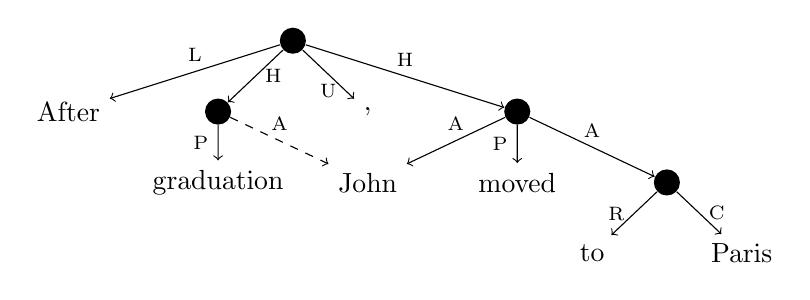
\begin{tikzpicture}[level distance=9mm, sibling distance=19mm, ->,
        every circle node/.append style={fill=black}]
      \tikzstyle{word} = [font=\rmfamily,color=black]
      \node (ROOT) [circle] {}
        child {node (After) [word] {After} edge from parent node[above] {\scriptsize L}}
        child {node (graduation) [circle] {}
        {
          child {node [word] {graduation} edge from parent node[left] {\scriptsize P}}
        } edge from parent node[right] {\scriptsize H} }
        child {node [word] {,} edge from parent node[below] {\scriptsize U}}
        child {node (moved) [circle] {}
        {
          child {node (John) [word] {John} edge from parent node[above] {\scriptsize A}}
          child {node [word] {moved} edge from parent node[left] {\scriptsize P}}
          child {node [circle] {}
          {
            child {node [word] {to} edge from parent node[left] {\scriptsize R}}
            child {node [word] {Paris} edge from parent node[right] {\scriptsize C}}
          } edge from parent node[above] {\scriptsize A} }
        } edge from parent node[above] {\scriptsize H} }
        ;
      \draw[dashed,->] (graduation) to node [above] {\scriptsize A} (John);
    \end{tikzpicture}
    }
\caption{UCCA graph. Dashed: remote edge.\label{fig:example_ucca}}
\end{figure}



%%%%%%%%%%%%%%%%%%%%%%%%%%%%%%%%%%%%%%%%%%%%%%%%%%%%%%%%%%%%%%%%
\paragraph{UD}\label{sec:udd}
is a syntactic dependency scheme used in many languages,
aiming for cross-linguistically consistent and coarse-grained treebank
annotation. Formally, UD uses bi-lexical trees, with edge labels 
representing syntactic relations.

  One aspect of UD similar to UCCA is its preference of lexical (rather than functional) heads.
  For example, in auxiliary verb constructions (e.g., ``is eating''), UD
  marks the lexical verb (\textit{eating}) as the head, while other dependency schemes
  may select the auxiliary \textit{is} instead.
  While the approaches are largely inter-translatable
  \citep{Schwartz:12}, lexical head schemes are more similar in form to semantic schemes,
   such as UCCA and semantic dependencies \citep{oepen2016towards}.
   
Being a dependency representation, UD is structurally underspecified in an important way:
​it is not possible in UD to mark the distinction between an element modifying the head of
the phrase and the same element modifying the whole phrase
\cite{doi:10.1146/annurev-linguistics-011718-011842}.
   
An example UD tree is given in Figure~\ref{fig:original_example_udd}.
UD relations will be written in \texttt{typewriter} font.

\begin{figure}[th]
  \centering
    \begin{dependency}[text only label, label style={above,font=\tt}, font=\small]
    \begin{deptext}[column sep=.8em,ampersand replacement=\^]
    After \^ graduation \^ , \^ John \^ moved \^ to \^ Paris \\
    \end{deptext}
        \depedge[edge unit distance=1ex]{2}{1}{case}
        \depedge[edge unit distance=1ex]{2}{3}{punct}
        \depedge[edge unit distance=1ex]{5}{4}{nsubj}
        \depedge[edge unit distance=1ex, edge end x offset=-2pt]{5}{2}{obl}
        \depedge[edge unit distance=1ex]{7}{6}{case}
        \deproot[edge unit distance=1.5ex]{5}{root}
        \depedge[edge unit distance=1.5ex]{5}{7}{obl}
    \end{dependency}
\caption{UD tree.\label{fig:original_example_udd}}
\end{figure}

%%%%%%%%%%%%%%%%%%%%%%%%%%%%%%%%%%%%%%%%%%%%%%%%%%%%%%%%%%%%%%%%%%%%%%%%%%%%%%%%%%%%%%%%%%%%%%
\section{Shared Gold-standard Corpus}\label{sec:shared}

We annotate 723 English passages (3,813 sentences; 52,721 tokens),
comprising the web reviews section of the 
English Web Treebank \cite[EWT; ][]{bies2012english}.
Text is annotated by two UCCA annotators
according to v2.0 of the UCCA
guidelines\footnote{\url{http://bit.ly/ucca_guidelines_v2}}
and cross-reviewed.
As these sentences are included in the UD
English\_EWT treebank, this is a \textit{shared} gold-standard UCCA and UD
annotated corpus.\footnote{Our data is available at \url{https://github.com/UniversalConceptualCognitiveAnnotation/UCCA_English-EWT}.}
We use the standard train/development/test split,
shown in Table~\ref{tab:data}.

\begin{table}[t]
\centering
\begin{tabular}{l|ccc}
& \bf \footnotesize Train & \bf \footnotesize Dev & \bf \footnotesize Test \\
\hline
\# Passages & \hphantom{00,}347 & \hphantom{0,}192 & \hphantom{0,}184 \\
\# Sentences & \hphantom{0}2,723 & \hphantom{0,}554 & \hphantom{0,}535 \\
\# Tokens & 44,804 & 5,394 & 5,381 \\
\end{tabular}
\caption{Data split for the shared gold-standard corpus.\label{tab:data}}
\end{table}

%%%%%%%%%%%%%%%%%%%%%%%%%%%%%%%%%%%%%%%%%%%%%%%%%%%%%%%%%%%%%%%%%%%%%%%%%%%%%%%%%%%%%%%%%%%%%%
\section{Comparison Methodology}\label{sec:methodology}

To facilitate comparison between UCCA and UD,
we first assimilate the graphs by abstracting away from formalism differences,
obtaining a similar graph format for both schemes.
We then match pairs of nodes in the converted UD and UCCA trees
if they share all terminals in their yields.

UD annotates bi-lexical dependency trees,
while UCCA graphs contain non-terminal nodes.
In \S\ref{sec:conversion}, we outline the unified DAG converter by
\citet{hershcovich2018multitask,hershcovich2018universal},\footnote{\url{https://github.com/huji-nlp/semstr}}
which we use to reach a common format.
In \S\ref{sec:local}, we describe a number of extensions
to the converter, which abstract away from further non-content differences.

\begin{figure}[th]
  \centering
  \scalebox{.8}{
  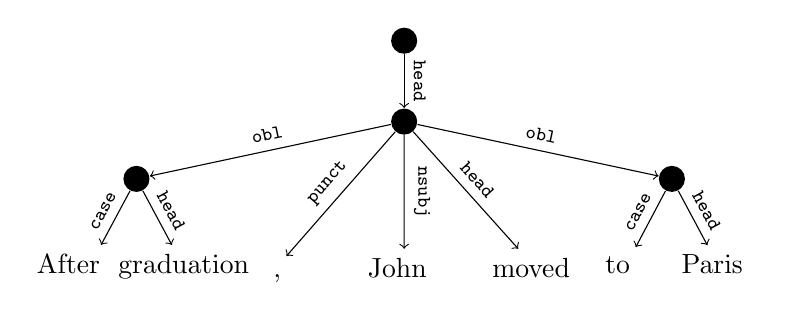
\begin{tikzpicture}[level distance=12mm, ->,
      every node/.append style={sloped,anchor=south,auto=false,font=\scriptsize\tt},
      level 2/.style={sibling distance=17mm,level distance=9mm},
      level 3/.style={sibling distance=12mm,level distance=14mm}]
    \tikzstyle{word} = [font=\rmfamily,color=black]
    \node [fill=black,circle] {}
      child {node (ROOT) [fill=black,circle] {}
      {
        child {node (after) [fill=black,circle] {}
        {
          child {node [word] {After{\color{white}g}\quad\quad} edge from parent node {case}}
          child {node [word] {\quad graduation\quad\quad} edge from parent node {head}}
        } edge from parent node {obl}}
        child {node {}
        {
          child {node [word] (comma) {\quad,{\color{white}g}} edge from parent [draw=none]}
        } edge from parent [draw=none]}
        child {node {}
        {
          child {node [word] (John) {John{\color{white}g}} edge from parent [draw=none]}
        } edge from parent [draw=none]}
        child {node {}
        {
          child {node [word] (moved) {moved{\color{white}g}} edge from parent [draw=none]}
        } edge from parent [draw=none]}
        child {node (to) [fill=black,circle] {}
        {
            child {node [word] {to{\color{white}g}} edge from parent node {case}}
            child {node [word] {Paris{\color{white}g}} edge from parent node {head}}
        } edge from parent node {obl}}
      } edge from parent node {head}}
      ;
      \draw (ROOT) to node {punct} (comma);
      \draw (ROOT) to node {nsubj} (John);
      \draw (ROOT) to node {head} (moved);
  \end{tikzpicture}}
\caption{Converted UD tree.
Non-terminals and \textit{head} edges are introduced by the unified DAG converter.\label{fig:converted_example_udd}}
\end{figure}


\subsection{Basic Conversion}\label{sec:conversion}

Figure~\ref{fig:converted_example_udd} presents the same tree from Figure~\ref{fig:original_example_udd}
after conversion.
The converter adds one pre-terminal per token,
and attaches them according to the original dependency tree:
traversing it from the root, for each head it creates a non-terminal
parent with the edge label {\it head}, and adds the dependents as children of 
the created non-terminal.
Relation subtypes are stripped,
leaving only universal relations.
For example, the language-specific definite article label
\texttt{det:def} is replaced by the universal \texttt{det}.

\paragraph{Reentrancies.}
Remote edges in UCCA enable reentrancy, forming a DAG together with primary edges.
UD allows reentrancy when including \textit{enhanced dependencies}
\cite{SCHUSTER16.779},\footnote{\url{https://universaldependencies.org/u/overview/enhanced-syntax.html}} which form (bi-lexical) graphs, representing phenomena
such as predicate ellipsis (e.g., gapping),
and shared arguments due to coordination, control, raising and relative clauses.

UCCA is more inclusive in its use of remote edges, and accounts for 
the entire class of implicit arguments termed {\it Constructional Null Instantiation} in FrameNet \citep{Ruppenhofer:16}.
For example, in
``The Pentagon is bypassing official US intelligence channels [...] in order to create strife'' (from EWT),
remote edges mark \textit{Pentagon} as a shared argument of \textit{bypassing} and
\textit{create}. 
Another example is ``if you call for an appointment [...] so you can then make one'',
where a remote edge in UCCA indicates that \textit{one} refers to \textit{appointment}.
Neither is covered by enhanced UD.

In order to facilitate comparison, we remove remote edges and enhanced dependencies in the conversion process.
We thus compare basic UD and UCCA trees, deferring a comparison of UCCA and enhanced UD to future work.



\subsection{Extensions to the Converter}\label{sec:local}

We extend the unified DAG converter to remove further non-content differences.

\paragraph{Unanalyzable units.}
An unanalyzable phrase is represented in UCCA as a single unit covering multiple terminals.
In multi-word expressions (MWEs) in UD, each word after the first is attached to the previous word,
with the \texttt{flat}, \texttt{fixed} or \texttt{goeswith} relations
(depending on whether the expression is grammaticalized, or split by error).
We remove edges of these relations and join the corresponding pre-terminals to one unit.

\paragraph{Promotion of conjunctions.}
The basic conversion generally preserves terminal yields:
the set of terminals spanned by a non-terminal is the same
as the original dependency yield of its head terminal
(e.g., in Figure~\ref{fig:converted_example_udd}, the yield of the non-terminal
headed by \textit{graduation} is ``After graduation'', the same as that of ``graduation''
in Figure~\ref{fig:original_example_udd}).

Since UD attaches subordinating and coordinating conjunctions to the subsequent conjunct,
this results in them being positioned in the same conjunct they relate (e.g.,
\textit{After} will be included in the first conjunct in ``After arriving home, John went to sleep'';
\textit{and} will be included in the second conjunct in ``John and Mary'').
In contrast, UCCA places conjunctions as siblings to their conjuncts (e.g.,
``[After] [arriving home], [John went to sleep]'' and ``[John] [and] [Mary]''). 

To abstract away from these convention differences,
we place 
coordinating and subordinating conjunctions 
(i.e., \texttt{cc}-labeled units, and \texttt{mark}-labeled units with an \texttt{advcl} head such 
as \textit{when}, \textit{if}, \textit{after}) as siblings of their conjuncts.


%%%%%%%%%%%%%%%%%%%%%%%%%%%%%%%%%%%%%%%%%%%%%%%%%%%%%%%%%%%%%%%%%%%%%%%%%%%%%%%
\section{Analysis of Divergences}\label{sec:analysis}

Using the shared format,
we turn to analyzing the content differences between UCCA and UD.\footnote{See
\url{http://bit.ly/uccaud} for a detailed explanation of each example in
this section.}


\begin{table*}[t]
\centering
\scalebox{.6}{
\setlength\tabcolsep{6.7pt}
\def\arraystretch{.815}
\begin{tabular}{lRRRRRRRRRRRRRRRR|R}
 &&&&&&&&&&&&&&&&& \multicolumn{1}{|c}{\sc No} \\
 & \multicolumn{1}{c}{\bf A}
 & \multicolumn{1}{c}{\bf A\big|P} & \multicolumn{1}{c}{\bf A\big|S}
 & \multicolumn{1}{c}{\bf C}
 & \multicolumn{1}{c}{\bf D}
 & \multicolumn{1}{c}{\bf E}
 & \multicolumn{1}{c}{\bf F}
 & \multicolumn{1}{c}{\bf G}
 & \multicolumn{1}{c}{\bf H}
 & \multicolumn{1}{c}{\bf L}
 & \multicolumn{1}{c}{\bf N}
 & \multicolumn{1}{c}{\bf P}
 & \multicolumn{1}{c}{\bf Q}
 & \multicolumn{1}{c}{\bf R}
 & \multicolumn{1}{c}{\bf S}
 & \multicolumn{1}{c}{\bf T}
 & \multicolumn{1}{|c}{\sc Match} \\
\tt acl & 58 &  &  & 1 & 4 & 249 & 1 &  & 48 &  &  & 6 &  &  & 1 & 1 & 409 \\
\tt advcl & 14 &  &  & 12 & 2 & 2 &  & 6 & 512 & 4 &  & 11 &  &  &  &  & 423 \\
\tt advmod & 225 &  & 1 & 69 & 1778 & 332 & 27 & 135 & 14 & 258 & 2 & 2 & 15 & 44 & 9 & 368 & 273 \\
\tt amod & 25 &  &  & 134 & 647 & 837 &  & 1 & 28 &  &  & 7 & 130 & 3 & 269 & 25 & 176 \\
\tt appos & 21 &  &  & 39 & 2 & 34 &  &  & 18 &  &  &  &  &  & 8 &  & 33 \\
\tt aux &  &  &  &  & 384 & 2 & 1335 &  &  & 2 &  & 1 &  & 1 &  &  & 17 \\
\tt case & 11 &  &  & 31 & 27 & 25 & 123 &  &  & 213 & 26 & 11 & 1 & 2629 & 154 & 1 & 262 \\
\tt cc &  &  &  & 8 & 4 & 1 & 4 & 1 & 1 & 1567 & 381 &  & 6 & 12 &  &  & 52 \\
\tt ccomp & 345 &  &  & 1 &  & 1 &  &  & 36 &  &  & 2 &  &  & 1 & 1 & 166 \\
\tt compound & 225 &  &  & 116 & 67 & 586 & 21 &  & 2 &  &  & 32 & 19 & 1 & 12 & 24 & 683 \\
\tt conj & 10 &  &  & 449 & 4 & 5 &  & 1 & 1262 & 1 &  & 6 & 2 &  & 10 &  & 497 \\
\tt cop &  &  &  & 1 &  &  & 1312 &  &  & 1 &  & 9 &  & 10 & 178 &  & 7 \\
\tt csubj & 13 &  &  &  &  &  &  &  & 3 &  &  &  &  &  &  &  & 46 \\
\tt det & 10 &  &  & 17 & 119 & 440 & 2963 &  &  &  & 1 &  & 129 & 16 & 1 &  & 124 \\
\tt discourse & 1 &  &  & 2 & 1 &  & 25 & 29 & 27 & 16 &  &  &  &  & 5 &  & 19 \\
\tt expl & 21 &  &  & 1 &  &  & 98 &  &  &  &  &  &  &  & 17 &  & 3 \\
\tt iobj & 131 &  &  & 1 &  &  & 1 &  &  &  &  &  &  &  &  &  & 10 \\
\tt list & 3 &  &  & 7 & 2 & 1 &  &  & 27 &  &  &  &  &  & 1 &  & 6 \\
\tt mark &  &  &  & 9 & 7 & 1 & 531 & 1 &  & 654 &  &  &  & 407 & 1 & 5 & 143 \\
\tt nmod & 844 & 1 & 1 & 20 & 9 & 786 & 8 & 4 & 12 & 1 & 1 & 20 & 2 & 2 & 11 & 27 & 488 \\
\tt nsubj & 4296 & 7 & 21 & 25 & 3 & 2 & 55 & 1 & 5 & 61 &  & 58 & 1 & 80 & 14 & 4 & 247 \\
\tt nummod & 2 &  &  & 33 & 12 & 17 &  & 4 &  & 4 &  &  & 334 &  &  &  & 64 \\
\tt obj & 1845 &  & 1 & 54 & 21 & 6 & 11 & 1 & 4 & 23 &  & 52 & 1 & 23 & 3 & 11 & 583 \\
\tt obl & 1195 &  &  & 19 & 115 & 41 & 1 & 17 & 39 & 34 &  & 6 & 6 & 26 & 7 & 302 & 611 \\
\tt parataxis & 6 &  & 1 & 5 &  & 4 &  & 6 & 285 &  &  &  &  &  & 3 &  & 180 \\
\tt vocative & 17 &  &  &  &  &  &  & 8 &  &  &  &  &  &  &  &  &  \\
\tt xcomp & 121 &  &  & 4 & 25 &  &  &  & 8 &  &  & 38 &  &  & 38 &  & 526 \\
\hline
head & 445 & 48 & 159 & 6388 & 717 & 142 & 564 & 83 & 2462 & 42 & 1 & 4163 & 120 & 52 & 1547 & 32 & 2235 \\
\hline
\sc No Match & 1421 & 37 & 58 & 640 & 417 & 291 & 14 & 33 & 2291 & 146 & 6 & 802 & 94 & 52 & 369 & 96 & 
\end{tabular}
}
\caption{UD-UCCA confusion matrix calculated based on EWT
gold-standard annotations from the training and development sets
(\S\ref{sec:shared}),
after applying our extended converter to UD (\S\ref{sec:methodology}),
by matching UD vertices and UCCA units with the same terminal yield.
The last column (row), labeled {\sc No Match}, shows the number of edges of each UD (UCCA) category
that do not match any UCCA (UD) unit.
Zero counts are omitted.\label{tab:confusion_matrix}}
\end{table*}

\subsection{Confusion Matrix}\label{sec:confusion}

Table~\ref{tab:confusion_matrix} presents the confusion matrix of categories between
the converted UD and UCCA, calculated over all sentences in the training and
development sets of the shared EWT reviews corpus.
We leave the test set out of this evaluation to avoid contamination for future
parsing experiments.

In case of multiple UCCA units with the same terminal yield (i.e., units with a single non-remote child),
we take the top category only, to avoid double-counting.
Excluding punctuation, this results in 60,434 yields in UCCA and
58,992 in UD.
Of these, 52,280 are common, meaning that a UCCA ``parser'' developed this way
would get a very high F1 score
of 87.6\%, if it is provided with the gold UCCA label for every converted edge.

Some yields still have more than one UCCA category associated with them,
due to edges with multiple categories ({\bf A\big|P} and {\bf A\big|S}).
For presentation reasons, 0.15\% of the UCCA units in the data
are not presented here, as they belong to rare (<~0.1\%)
multiple-category combinations.

Only 82.6\% of UD's syntactic arguments
(\texttt{ccomp}, \texttt{csubj}, \texttt{iobj}, \texttt{nsubj}, \texttt{obj}, \texttt{obl} and \texttt{xcomp})
are UCCA Participants,
and only 72.9\% of the Participants are syntactic arguments---a difference stemming from
the Scene/non-Scene (\S\ref{sec:s}) and argument/adjunct (\S\ref{sec:arguments}) distinctions.
Moreover, if we identify predicates as words having at least one argument
and Scenes as units with at least one Participant,
then only 92.1\% of UD's predicates correspond to Scenes (many are secondary relations within one scene),
and only 80\% of Scenes correspond to predicates (e.g., eventive nouns,
which are not syntactic predicates).

Examining the {\it head} row in Table~\ref{tab:confusion_matrix} allows
us to contrast the schemes' notions of a head. 
{\it head}-labeled units have at least
one dependent in UD, or are single-clause sentences (technically, they are non-terminals added by the converter).
Of them, 75.7\% correspond to Processes, States, Parallel Scenes or Centers,
which are UCCA's notions of semantic heads,
and 11.6\% are left unmatched, mostly due to MWEs analyzed in
UD but not in UCCA (\S\ref{sec:mwe}).
Another source of unmatched units is inter-Scene linkage, which tends to be flatter in
UCCA (\S\ref{sec:linkage}).
The rest are mostly due to head swap (e.g., ``\textit{all} of Dallas'', where \textit{all}
is a Quantifier of \textit{Dallas} in UCCA, but the head in UD).

In the following subsections, we review the main content differences between the schemes,
as reflected in the confusion matrix, and categorize them according to the UD relations
involved.

\subsection{Scenes vs. Non-Scenes}\label{sec:s}

UCCA distinguishes between Scenes and non-Scenes.
This distinction crosses UD categories,
as a Scene can be evoked by a verb, an eventive or stative
noun (\textit{negotiation}, \textit{fatigue}),
an adjective or even a preposition (``this is \textit{for} John'').

\paragraph{Core syntactic arguments.}
      Subjects and objects are usually Participants (e.g., ``\textit{wine} was excellent'').
      However, when describing a Scene, the subject may be a Process/State
      (e.g., ``but \textit{service} is very poor'').
      Some wh-pronouns are the subjects or objects of a relative clause, but
      are Linkers or Relators,
      depending on whether they link Scenes or non-Scenes, respectively.
      For example, ``who'' in ``overall, Joe is a happy camper \textit{who} has found a great spot'' is an \texttt{nsubj}, but a Linker.
      Other arguments are Adverbials or Time (see \S\ref{sec:arguments}), and
      some do not match any UCCA unit, especially when they are parts of MWEs (see \S\ref{sec:mwe}).

\paragraph{Adjectival modifiers} are Adverbials when modifying Scenes
    (``\textit{romantic} dinner''), States when describing non-Scenes (``\textit{beautiful} hotel'') 
    or when semantically predicative (``such a \textit{convenient} location''), or
    Elaborators where defining inherent properties of non-Scenes (``\textit{medical} school'').

\paragraph{Nominal and clausal modifiers.}
    Most are Participants or Elaborators,
    depending on whether they modify a Scene (e.g.,
    ``discount \textit{on services}'' and
    ``our decision \textit{to buy when we did}'' are Participants,
    but ``\textit{my car's} gears and brakes'' and ``Some of the younger kids \textit{that work there}'' are Elaborators).
    Unmatched \texttt{acl} are often
    free relative clauses (e.g., in ``the prices were worth what \textit{I got}'',
    \textit{what} is the \texttt{obj} of \textit{worth} but
    a Participant of \textit{I got}).

\paragraph{Case markers.}
      While mostly Relators
      modifying non-Scenes (e.g., ``the team \textit{at} Bradley Chevron''),
      some case markers are Linkers linking Scenes together 
      (e.g., ``very informative website \textit{with} a lot of good work'').
      Others are Elaborators (e.g., ``\textit{over} a year'') or States
      when used as the main relation in verbless or copula clauses
      (e.g., ``it is right \textit{on} Wisconsin Ave'').
    
\paragraph{Coordination.}
      Coordinating conjunctions (\texttt{cc}) are Connectors where they coordinate non-Scenes
      (e.g., ``Mercedes \textit{and} Dan'')
      or Linkers where they coordinate Scenes (e.g., ``outdated \textit{but} not bad'').
      Similarly, conjuncts and list elements (\texttt{conj}, \texttt{list}) may be Parallel Scenes (H),
      or Centers when they are non-Scenes.\footnote{While in UD 
      the conjunction \texttt{cc} is attached to the following conjunct,
      in UCCA coordination is a flat structure.
      This is a convention difference that we normalize (\S\ref{sec:local}).}

\paragraph{Determiners.}
      Articles are Functions,
      but determiners modifying non-Scenes are Elaborators
      (e.g., ``I will never recommend this gym to \textit{any} woman'').
      Where modifying Scenes (mostly negation)
      they are marked as Adverbials. For example, ``\textit{no} feathers in stock'', ``\textit{what} a mistake'',
      and ``the rear window had \textit{some} leakage'' are all Adverbials.



\subsection{Primary and Secondary Relations}\label{sec:arguments}

UD distinguishes core arguments, adverb modifiers,
and obliques (in English UD, the latter mostly correspond to prepositional dependents of verbs).
UCCA distinguishes Participants, including locations and abstract entities,
from secondary relations (Adverbials), 
which cover manner, aspect and modality.
Adverbials can be verbs (e.g., \textit{begin}, \textit{fail}),
prepositional phrases (\textit{with disrespect}),
as well as modals, adjectives and adverbs.

\paragraph{Adverbs and obliques.}
    Most UD adverb modifiers are Adverbials (e.g., ``I \textit{sometimes} go''),
    but they may be Participants, mostly in the case of semantic arguments describing location (e.g., \textit{here}).
    Obliques
    may be
    Participants (e.g., ``wait \textit{for Nick}''), Time (e.g., ``for \textit{over 7 years}'') 
    or Adverbials---mostly manner adjuncts (\textit{by far}).

\paragraph{Clausal arguments}
    are Participant Scenes
    (e.g., ``it was great \textit{that they did not charge a service fee}'',
    ``did not really know \textit{what I wanted}'' or
    ``I asked them \textit{to change it}'').
    However, when serving as complements to a secondary verb, they
    will not match any unit in UCCA, as it places secondary verbs on the 
    same level as their primary relation. 
    For example, \textit{to pay} is an \texttt{xcomp} in ``they have to pay'', while
    the UCCA structure is flat: \textit{have to} is an Adverbial and \textit{pay} is a Process.
    Single-worded clausal arguments may correspond to a Process/State,
    as in ``this seems \textit{great}''.

\paragraph{Auxiliary verbs}
    are Functions (e.g., ``\textit{do} not forget''),
    or Adverbials when they are modals (e.g., ``you \textit{can} graduate''). Semi-modals 
    in UD are treated as clausal heads, which take a clausal complement. 
    For example, in ``able to do well'', UD treats \textit{able} as the head,
    which takes \textit{do well} as an \texttt{xcomp}. UCCA, on the other hand,
    treats it as an Adverbial, creating a mismatch for \texttt{xcomp}.
    

\subsection{Multi-Word Expressions}\label{sec:mwe}

UD and UCCA treat MWEs differently.
In UD they include names, compounds and grammaticalized fixed expressions.
UCCA treats names and grammaticalized MWEs as unanalyzable units,
but also a range of semantically opaque constructions
(e.g., light verbs and idioms).
On the other hand, compounds are not necessarily unanalyzable in UCCA,
especially if compositional.

\paragraph{Compounds.} English compounds are mostly nominal,
        and are a very heterogeneous category.
        Most compounds correspond to Elaborators (e.g., ``\textit{industry} standard''),
        or Elaborator Scenes (e.g., ``\textit{out-of-place} flat-screen TV''),
        and many are unanalyzable expressions (e.g., ``\textit{mark} up'').
        Where the head noun evokes a Scene, the dependent is often a Participant
        (e.g., ``\textit{food} craving''), but can also be an Adverbial 
        (e.g., ``\textit{first time} buyers'') depending on its semantic category.
        Other compounds in UD are phrasal verbs (e.g., ``figure \textit{out}'', ``cleaned \textit{up}''),
        which UCCA treats as unanalyzable (leading to unmatched units). 
            
\paragraph{Core arguments.}
      A significant number of subjects and objects are left unmatched as they
      form parts of MWEs marked in UCCA as unanalyzable. UD annotates
      MWEs involving a verb and its argument(s) just like any other clause, and therefore
      lacks this semantic content. Examples include light verbs (e.g., ``give {\it a try}''),
      idioms (``bites {\it the dust}''), and figures of speech (e.g., ``when \textit{it} comes to'', ``offer \textit{a taste} (of)''),
      all are UCCA units.
      
\paragraph{Complex prepositions.} Some complex prepositions (e.g., \textit{according to} or \textit{on top of}),
      not encoded as MWEs in UD, are unanalyzable in UCCA.


\subsection{Linkage}\label{sec:linkage}

\paragraph{Head selection.}
UCCA tends to flatten linkage, where UD, as a dependency scheme,
selects a head and dependent per relation.
This yields scope ambiguities for coordination, an inherently flat structure. 
For instance, ``unique gifts and cards'' is ambiguous in UD as to whether
\textit{unique} applies only to \textit{gifts} or to the whole phrase---both
annotated as in Figure~\ref{fig:conj_ud}.
UCCA, allowing non-terminal nodes, disambiguates this case (Figure~\ref{fig:conj_ucca}).

\begin{figure}[th]
  \centering
\begin{subfigure}{.4\columnwidth}\centering
    \begin{dependency}[text only label, label style={above,font=\tt}, font=\small, edge unit distance=1.5ex]
    \begin{deptext}[column sep=.1em,ampersand replacement=\^]
    unique \^ gifts \^ and \^ cards \\
    \end{deptext}
        \depedge{2}{1}{amod}
        \deproot{2}{root}
        \depedge{4}{3}{cc}
        \depedge{2}{4}{conj}
    \end{dependency}
    \caption{UD\label{fig:conj_ud}}
\end{subfigure}
\hfill
\begin{subfigure}{.4\columnwidth}\centering
    \scalebox{.8}{
    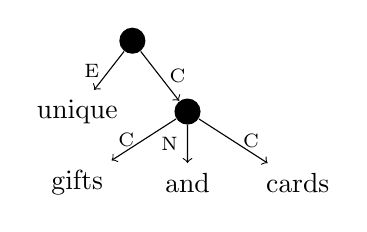
\begin{tikzpicture}[level distance=9mm, sibling distance=14mm, ->,
        every circle node/.append style={fill=black}]
      \tikzstyle{word} = [font=\rmfamily,color=black]
      \node (ROOT) [circle] {}
        child {node [word] {unique} edge from parent node[left] {\scriptsize E}}
        child {node [circle] {}
        {
          child {node [word] {gifts} edge from parent node[left] {\scriptsize C}}
          child {node [word] {and} edge from parent node[left] {\scriptsize N}}
          child {node [word] {cards} edge from parent node[right] {\scriptsize C}}
        } edge from parent node[right] {\scriptsize C} }
        ;
    \end{tikzpicture}
    }
    \caption{UCCA\label{fig:conj_ucca}}
 \end{subfigure}
 \caption{Coordination in UD and UCCA.\label{fig:conj}}
\end{figure}


\paragraph{Clausal dependents.}
UD categorizes clause linkage into coordination,
subordination, argumenthood (complementation),
and parataxis. %(a residual category).
UCCA distinguishes argumenthood 
but conflates the others into the Parallel Scene category.
For example,
``We called few companies before \textit{we decided to hire them}''
and ``Check out The Willow Lounge, \textit{you'll be happy}'' are Parallel Scenes.

Note that while in UD, \texttt{mark} (e.g., \textit{before})
is attached to the dependent adverbial clause,
a UCCA Linker lies outside the linked Scenes.
To reduce unmatched \texttt{advcl} instances,
this convention difference is fixed by the converter
(\S\ref{sec:local}).
Many remaining unmatched units are due to conjunctions we could not reliably raise.
For instance, the marker \textit{to} introducing an \texttt{xcomp} is ambiguous between Linker
(purposive \textit{to}) and Function (infinitive marker).
Similarly, wh-pronouns may be Linkers
(``he was willing to budge a little on the price {\it which} means a lot to me''),
but have other uses in questions and free relative clauses.
Other mismatches result from the long tail of differences in how UD and UCCA construe linkage.
Consider the sentence in Figure~\ref{fig:linkage}.
While \textit{moment} is an oblique argument of \textit{know} in UD,
\textit{From the moment} is analyzed as a Linker in UCCA.

\begin{figure}[th]\centering
\begin{subfigure}{\columnwidth}\centering
  \begin{minipage}[c]{.12\textwidth}
    \caption{UD\label{fig:linkage_ud}}
  \end{minipage}
  \begin{minipage}[c]{.8\textwidth}\centering
    \begin{dependency}[text only label, label style={above,font=\tt}, font=\small, edge unit distance=1.8ex]
    \begin{deptext}[column sep=.6em,ampersand replacement=\^]
    From \^ the \^ moment \^ you \^ enter \^ , \^ you \^ know \\
    \end{deptext}
        \depedge[edge unit distance=2.4ex]{3}{1}{case}
        \depedge{3}{2}{det}
        \depedge[edge unit distance=1ex]{8}{3}{obl}
        \depedge[edge unit distance=1.5ex]{3}{5}{acl}
        \depedge[edge start x offset=-5pt,edge unit distance=1ex]{5}{4}{nsubj}
        \depedge[edge unit distance=1.5ex]{8}{6}{punct}
        \depedge[edge start x offset=-10pt,edge unit distance=1ex]{8}{7}{nsubj}
        \deproot{8}{root}
    \end{dependency}
  \end{minipage}
\end{subfigure}

\begin{subfigure}{\columnwidth}\centering
  \begin{minipage}[c]{.17\textwidth}
    \caption{UCCA\label{fig:linkage_ucca}}
  \end{minipage}
  \hspace{-8mm}
  \begin{minipage}[c]{.8\textwidth}\centering
    \scalebox{.8}{
    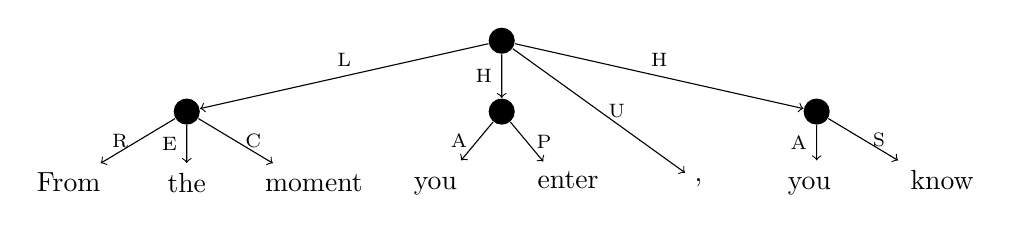
\begin{tikzpicture}[level distance=9mm, sibling distance=4cm, ->,
        level 2/.style={sibling distance=15mm},
        every circle node/.append style={fill=black}]
      \tikzstyle{word} = [font=\rmfamily,color=black]
      \node (ROOT) [circle] {}
        child {node [circle] {}
        {
          child {node [word] {From} edge from parent node[left] {\scriptsize R}}
          child {node [word] {the} edge from parent node[left] {\scriptsize E}}
          child {node [word] {{\color{white}F}moment} edge from parent node[right] {\scriptsize C}}
        } edge from parent node[above] {\scriptsize L} }
        child {node [circle] {}
        {
          child {node [word] {you{\color{white}k}} edge from parent node[left] {\scriptsize A}}
          child {node [word] {{\color{white}y}enter} edge from parent node[right] {\scriptsize P}}
        } edge from parent node[left] {\scriptsize H} }
        child {node [circle] {}
        {
          child {node (comma) [word] {,} edge from parent [draw=none]}
          child {node [word] {you{\color{white}k}} edge from parent node[left] {\scriptsize A}}
          child {node [word] {{\color{white}y}know} edge from parent node[right] {\scriptsize S}}
        } edge from parent node[above] {\scriptsize H} }
        ;
      \draw[->] (ROOT) to node [right] {\scriptsize U} (comma);
    \end{tikzpicture}
    }
  \end{minipage}
 \end{subfigure}
 \caption{Clause linkage in UD and UCCA.\label{fig:linkage}}
\end{figure}
    

\subsection{Other Differences}\label{sec:misc}

\paragraph{Appositions}
    in UD always follow the modified noun,
    but named entities in them are UCCA Centers, regardless of position
    (e.g., in ``its sister store Peking Garden'', the UD head \textit{its sister store}
    is an Elaborator, while \textit{Peking Garden} is the Center).

\paragraph{Copulas.}
    UCCA distinguishes copular constructions expressing
    identity (e.g., ``This \textit{is} the original Ham's restaurant'') where the copula is annotated as State,
    and cases of attribution 
    (e.g., ``Mercedes and Dan \textit{are} very thorough'')
    or location (e.g., ``Excellent chefs \textit{are} in the kitchen''),
    where the copula is a Function.

\paragraph{Discourse markers and interjections.}
    Units relating a Scene to the speech event or to the speaker's opinion are Ground
    (e.g., ``\textit{no}, Warwick in New Jersey'' and ``\textit{Please} visit my website'').
    On the other hand, discourse elements that relate one Scene to another 
    are Linkers (e.g., \textit{anyway}).

\paragraph{Vocatives}
    are both Ground and Participants if they participate in the Scene \textit{and} are the party addressed.
    For example, \textit{Mark} in ``Thanks \textit{Mark}'' is both the person addressed and the one thanked.\footnote{The {\bf A\big|G} column is omitted from
    Table~\ref{tab:confusion_matrix} as this category combination
    occurs in only 0.02\% of edges in the corpus.}
    
\paragraph{Expletives and subjects.}
    Expletives are generally Functions,
    but some instances of \textit{it} and \textit{that} are analyzed as \texttt{nsubj} in UD
    and as Function in UCCA (e.g., ``\textit{it}'s like driving a new car'').

\paragraph{Excluded relations.}
We exclude the following UD labels,
as they are irrelevant to our evaluation:
\texttt{root} (always matches the entire sentence);
\texttt{punct} (punctuation is ignored in UCCA evaluation);
\texttt{dep} (unspecified dependency),
\texttt{orphan} (used for gapping, which is represented using remote edges in UCCA---see \S\ref{sec:conversion});
\texttt{fixed}, \texttt{flat} and \texttt{goeswith} (correspond to parts of unanalyzable units in UCCA,
    and so do not represent units on their own---see \S\ref{sec:local});
    \texttt{reparandum} and \texttt{dislocated} (too rare in EWT).
    

%%%%%%%%%%%%%%%%%%%%%%%%%%%%%%%%%%%%%%%%%%%%%%%%%%%%%%%%%%%%%%%%%%%%%%%%%%%%%%%%%
\section{Fine-Grained UCCA Parsing Evaluation}\label{sec:fine_grained}

In \S\ref{sec:analysis} we used our comparison methodology,
consisting of the conversion to a shared format and matching units by terminal yield,
to compare gold-standard UD and UCCA.
In this section we apply the same methodology to parser outputs,
using gold-standard UD for fine-grained evaluation.

\subsection{Experimental Setup}\label{sec:experiments}

\paragraph{Data.}

In addition to the UCCA EWT data (\S\ref{sec:shared}),
we use the reviews section of the UD v2.3 English\_EWT treebank
\cite{11234/1-2895},\footnote{\url{https://hdl.handle.net/11234/1-2895}}
annotated over the exact same sentences.
We additionally use UDPipe v1.2 \cite{udpipe,udpipe:2017},
trained on
English\_EWT,\footnote{\url{https://hdl.handle.net/11234/1-2898}}
for feature extraction.
We apply the extended converter to UD as before (\S\ref{sec:local}).

\paragraph{Parser.}

We train TUPA v1.3 \cite{hershcovich2017a,hershcovich2018multitask}
on the UCCA EWT data, with the standard train/development/test split.
TUPA uses POS tags and syntactic dependencies as features.
We experiment both with using gold UD for feature extraction,
and with using UDPipe outputs.


\paragraph{Evaluation by gold-standard UD.}

UCCA evaluation is generally carried out by considering a predicted unit as correct if there
is a gold unit that matches it in terminal yield and labels. Precision, Recall and F-score (F1)
are computed accordingly.
For the fine-grained analysis, we split the gold-standard, predicted and matched UCCA units according
to the labels of the UD relations whose dependents have the same terminal yield (if any).


\subsection{Results}\label{sec:results}

Table~\ref{tab:results} presents TUPA's scores on the UCCA EWT development
and test sets. Surprisingly, using UDPipe for feature extraction results in
better scores than gold syntactic tags and dependencies.

\begin{table}[h]\centering
\begin{tabular}{llll|lll}
& \multicolumn{3}{c|}{\footnotesize \bf Primary} & \multicolumn{3}{c}{\footnotesize \bf Remote} \\
\multicolumn{1}{l}{\footnotesize \bf Features}
& \footnotesize \textbf{LP} & \footnotesize \textbf{LR} & \footnotesize \textbf{LF}
& \footnotesize \textbf{LP} & \footnotesize \textbf{LR} & \footnotesize \textbf{LF} \\
\hline
\multicolumn{4}{@{}l|}{\footnotesize Development} \\
\multicolumn{1}{l}{\footnotesize Gold UD}
 & 72.1 & 71.2 & 71.7 & 61.2 & 38.1 & 47.0 \\
\multicolumn{1}{l}{\footnotesize UDPipe} 
 & 73.0 & 72.1 & 72.5 & 53.7 & 40.8 & 46.4 \\
\hline
\multicolumn{4}{@{}l|}{\footnotesize Test} \\
\multicolumn{1}{l}{\footnotesize Gold UD}
 & 72.2 & 71.2 & 71.7 & 60.9 & 36.8 & 45.9 \\
\multicolumn{1}{l}{\footnotesize UDPipe} 
 & 72.4 & 71.7 & 72.1 & 60.3 & 38.5 & 47.0
\end{tabular}
\caption{
Labeled precision, recall and F1 (in~\%) for primary and
remote edges output by TUPA on the UCCA EWT development (top) and test (bottom)
sets, using either gold-standard UD or UDPipe for TUPA features.\label{tab:results}}
\end{table}

\begin{table*}[t]
\centering
\scriptsize
\setlength\tabcolsep{.3pt}
\def\arraystretch{1.2}
\hspace{-2mm}
\begin{tabular}{cl|rrrrrrrrrrrrrrrrrrrrrrrrrrr}
 &  & \multicolumn{1}{c}{\scriptsize \tt \rotatebox{90}{aux}} & \multicolumn{1}{c}{\scriptsize \tt \rotatebox{90}{det}} & \multicolumn{1}{c}{\scriptsize \tt \rotatebox{90}{cop}} & \multicolumn{1}{c}{\scriptsize \tt \rotatebox{90}{cc}} & \multicolumn{1}{c}{\scriptsize \tt \rotatebox{90}{expl}} & \multicolumn{1}{c}{\scriptsize \tt \rotatebox{90}{iobj}} & \multicolumn{1}{c}{\scriptsize \tt \rotatebox{90}{nsubj}} & \multicolumn{1}{c}{\scriptsize \tt \rotatebox{90}{case}} & \multicolumn{1}{c}{\scriptsize \tt \rotatebox{90}{list}} & \multicolumn{1}{c}{\scriptsize \tt \rotatebox{90}{advmod}} & \multicolumn{1}{c}{\scriptsize \tt \rotatebox{90}{amod}} & \multicolumn{1}{c}{\scriptsize \tt \rotatebox{90}{nummod}} & \multicolumn{1}{c}{\scriptsize \tt \rotatebox{90}{mark}} & \multicolumn{1}{c}{\scriptsize \tt \rotatebox{90}{vocative}} & \multicolumn{1}{c}{\scriptsize \tt \rotatebox{90}{compound}} & \multicolumn{1}{c}{\scriptsize \tt \rotatebox{90}{obj}} & \multicolumn{1}{c}{\scriptsize \tt \rotatebox{90}{nmod}} & \multicolumn{1}{c}{\scriptsize \tt \rotatebox{90}{conj}} & \multicolumn{1}{c}{\scriptsize \tt \rotatebox{90}{advcl}} & \multicolumn{1}{c}{\scriptsize \tt \rotatebox{90}{obl}} & \multicolumn{1}{c}{\scriptsize \tt \rotatebox{90}{xcomp}} & \multicolumn{1}{c}{\scriptsize \tt \rotatebox{90}{discourse}} & \multicolumn{1}{c}{\scriptsize \tt \rotatebox{90}{ccomp}} & \multicolumn{1}{c}{\scriptsize \tt \rotatebox{90}{parataxis}} & \multicolumn{1}{c}{\scriptsize \tt \rotatebox{90}{appos}} & \multicolumn{1}{c}{\scriptsize \tt \rotatebox{90}{acl}} & \multicolumn{1}{c}{\scriptsize \tt \rotatebox{90}{csubj}} \\ \hline
\multirow{2}{*}{\footnotesize (a)} & \scriptsize \bf Labeled F1 \% & 94 & 93 & 89 & 86 & 83 & 83 & 80 & 76 & 76 & 72 & 71 & 71 & 70 & 62 & 59 & 57 & 55 & 50 & 49 & 48 & 41 & 38 & 29 & 23 & 21 & 20 & 0 \\
 & \scriptsize \bf Unlabeled F1 \% & 99 & 99 & 100 & 99 & 100 & 83 & 84 & 95 & 76 & 95 & 95 & 86 & 97 & 92 & 84 & 65 & 77 & 61 & 51 & 61 & 63 & 95 & 29 & 36 & 48 & 37 & 33 \\ \hline
\multirow{5}{*}{\footnotesize (b)} & \scriptsize \bf Total in UD \# & 156 & 392 & 187 & 212 & 12 & 8 & 463 & 335 & 15 & 378 & 374 & 38 & 116 & 1 & 219 & 222 & 231 & 244 & 52 & 208 & 1 & 16 & 29 & 52 & 22 & 81 & 5 \\
 & \scriptsize \bf Match Gold \# & 156 & 385 & 187 & 206 & 12 & 6 & 468 & 305 & 12 & 359 & 361 & 33 & 111 & 7 & 146 & 187 & 198 & 210 & 40 & 162 & 28 & 10 & 20 & 48 & 17 & 56 & 4 \\
 & \scriptsize \bf Match Predicted \# & 154 & 388 & 187 & 203 & 12 & 6 & 446 & 313 & 9 & 345 & 339 & 32 & 113 & 6 & 136 & 163 & 183 & 177 & 30 & 147 & 26 & 11 & 15 & 30 & 12 & 36 & 2 \\
 & \scriptsize \bf Labeled Correct \# & 145 & 361 & 166 & 175 & 10 & 5 & 365 & 236 & 8 & 253 & 248 & 23 & 78 & 4 & 83 & 99 & 104 & 96 & 17 & 74 & 11 & 4 & 5 & 9 & 3 & 9 & 0 \\
 & \scriptsize \bf Unlabeled Correct \# & 154 & 381 & 187 & 203 & 12 & 5 & 386 & 293 & 8 & 336 & 334 & 28 & 109 & 6 & 118 & 113 & 147 & 119 & 18 & 94 & 17 & 10 & 5 & 14 & 7 & 17 & 1 \\ \hline
\multirow{2}{*}{\footnotesize (c)} & \scriptsize \bf Labeled/Unlabeled \% & 94 & 95 & 89 & 86 & 83 & 100 & 95 & 81 & 100 & 75 & 74 & 82 & 72 & 67 & 70 & 88 & 71 & 81 & 94 & 79 & 65 & 40 & 100 & 64 & 43 & 53 & 0 \\
 & \scriptsize \bf Mode/Match Gold \% & 79 & 82 & 86 & 75 & 58 & 100 & 91 & 79 & 83 & 51 & 35 & 85 & 45 & 71 & 54 & 91 & 51 & 70 & 92 & 68 & 44 & 30 & 94 & 98 & 41 & 72 & 100 \\ \hline
\footnotesize (d) & \scriptsize \bf Average Words \# & 1.0 & 1.0 & 1.0 & 1.0 & 1.0 & 1.1 & 1.6 & 1.0 & 2.2 & 1.2 & 1.2 & 1.1 & 1.0 & 1.6 & 1.2 & 3.0 & 2.4 & 5.8 & 6.6 & 3.8 & 6.0 & 1.1 & 9.0 & 6.7 & 4.0 & 5.6 & 7.5
\end{tabular}
\caption{Fine-grained evaluation of TUPA (with gold-standard UD features) on the
EWT development set.
(a) Columns are sorted by labeled F1, measuring performance on each subset of edges.
Unlabeled F1 ignores edge categories, evaluating unit boundaries only.
(b) Total number of instances of each UD relation;
of them, matching UCCA units in gold-standard and in TUPA's predictions;
their intersection, with/without regard to categories.
(c) 
Percentage of correctly categorized edges;
for comparison, percentage of most frequent category (see~Table~\ref{tab:confusion_matrix}).
(d) Average number of words in corresponding terminal yields.\label{tab:fine_grained_results}}
\end{table*}

Table~\ref{tab:fine_grained_results} shows
fine-grained evaluation by UD relations.
TUPA does best on auxiliaries and determiners,
despite the heterogeneity of corresponding UCCA categories
(see Table~\ref{tab:confusion_matrix}),
possibly by making lexical distinctions
(e.g., modals and auxiliary verbs are both UD auxiliaries,
but are annotated as Adverbials and Functions, respectively).

Copulas and coordinating conjunctions pose a more difficult distinction,
since the same lexical items may have different categories depending on the
context: State/Function for copulas,
due to the distinction between identity and attribution, and
Connector/Linker for conjunctions,
due to the distinction between Scenes and non-Scenes.
However, the reviews domain imposes a strong prior for both (Function and Linker,
respectively), which TUPA learns successfully.

Inter-clause linkage (\texttt{conj}, \texttt{advcl}, \texttt{xcomp},
\texttt{ccomp}, \texttt{parataxis}, \texttt{acl} and \texttt{csubj})
is a common source of error for TUPA.
Although the match between UCCA and UD is not perfect in these cases,
it is overall better than TUPA's unlabeled performance,
despite using gold-standard syntactic features.
Our results thus suggest that encoding syntax more directly, perhaps using syntactic
scaffolding \citep{swayamdipta2018syntactic}
or guided attention \citep{strubell2018linguistically},
may assist in predicting unit boundaries.
However, TUPA often succeeds at making distinctions that are not even encoded in UD.
For example, it does reasonably well (71\%) on distinguishing between noun modifiers of
Scene-evoking nouns (Participants) and modifiers of other nouns (Elaborators),
surpassing a majority baseline based on the UD relation (51\%).
Lexical resources that distinguish eventive and relational nouns from concrete 
nouns may allow improving it even further.
In the similar case of compounds, lexical resources for light verbs and idioms may increase performance.


%%%%%%%%%%%%%%%%%%%%%%%%%%%%%%%%%%%%%%%%%%%%%%%%%%%%%%%%%%%%%%%%%%%%%%%%%%%%%%%%%
\section{Discussion}\label{sec:discussion}

NLP tasks
often require semantic distinctions that are difficult to extract from syntactic representations.
Consider the example
``after graduation, John moved to Paris'' again.
While \textit{graduation} evokes a Scene
(Figure~\ref{fig:example_ucca}), in UD it is an oblique modifier of \textit{moved},
just like \textit{Paris} is (Figure~\ref{fig:original_example_udd}).
The Scene/non-Scene distinction (\S\ref{sec:s})
would assist structural text simplification systems
in paraphrasing this sentence to two sentences, each one
containing one Scene \cite{sulem2018semantic}.

Another example is machine translation---translating the same sentence into Hebrew,
which does not have a word for \textit{graduation},
would require a clause to convey the same meaning.
The mapping would therefore be more direct using a semantic representation,
and we would benefit from breaking the utterance into two Scenes.


%%%%%%%%%%%%%%%%%%%%%%%%%%%%%%%%%%%%%%%%%%%%%%%%%%%%%%%%%%%%%%%%%%%%%%%%%%%%%%%%%
\section{Related Work}\label{sec:related_work}

The use of syntactic parsing as a proxy for semantic structure has a long tradition in NLP.
Indeed, semantic parsers have leveraged syntax
for output space pruning \cite{xue2004calibrating}, 
syntactic features \cite{gildea2002automatic,hershcovich2017a}, 
joint modeling \cite{surdeanu2008conll,hajivc2009conll}, and
multi-task learning \cite{swayamdipta2016greedy,swayamdipta2018syntactic,hershcovich2018multitask}.
Empirical comparison between syntactic and semantic schemes, however,
is still scarce.
\newcite{W14-2908} mapped Stanford Dependencies
(precursor to UD) to Hobbsian Logical Form, identifying semantic gaps in the former.
PredPatt \citep{white2016universal},
a framework for extracting predicate-argument structures from UD,
was evaluated by \newcite{zhang2017evaluation}
on a large set of converted PropBank annotations.
\newcite{szubert2018structured} proposed a method for aligning AMR and UD subgraphs,
finding that 97\% of AMR edges are evoked by one or more
words or syntactic relations.
\newcite{damonte-17} refined AMR evaluation by UD labels,
similar to our fine-grained evaluation of UCCA parsing.

Some syntactic representation approaches, notably CCG \cite{Steedman:00},
directly reflect the underlying semantics, and have been used to
transduce semantic forms using rule-based systems \cite{Basile:12}.
A related line of work tackles the transduction of syntactic structures into semantic ones.
\newcite{reddy2016transforming} proposed a rule-based method for converting UD
to logical forms.
\newcite{stanovsky2016getting} converted Stanford dependency trees into
proposition structures ({\sc PropS}), abstracting away from some syntactic detail.

\section{Conclusion}\label{sec:conclusion}

We evaluated the similarities and divergences in the content encoded by UD and UCCA. 
We annotated the reviews section of the English Web Treebank with UCCA,
  and used an automated methodology to evaluate how well the two schemes align,
  abstracting away from differences of mere convention.
We provided a detailed picture of the content differences between the schemes.
Notably, we quantified the differences between the notions of syntactic and semantic heads
  and arguments, finding substantial divergence between them.
Our findings highlight the potential utility of using semantic parsers for text understanding applications
  (over their syntactic counterparts), but also expose challenges semantic parsers must address,
  and potential approaches for addressing them.

\section*{Acknowledgments}

This work was supported by the Israel Science Foundation (grant No. 929/17),
and by the HUJI Cyber Security Research Center
in conjunction with the Israel National Cyber Bureau in the Prime Minister's Office.
We thank Jakob Prange, Nathan Schneider
and the anonymous reviewers for their helpful comments.





\chapter{Discussion}

In this thesis, I showed that meaning representation is valuable for language understanding,
and that TUPA, an accurate UCCA parser, is suited to many meaning representations.
Furthermore, multitask learning allows useful shared generalizations to emerge,
improving TUPA's performance by taking advantage of its general transition-based
architecture and flexible neural network classifier.
As different meaning representations capture many similar distinctions,
this approach proved effective, gaining from data annotated in each scheme
even though they had been designed separately and with different formal properties.
While divergences between the content of the schemes may limit the gain from sharing,
they highlight relative strengths, which are meaningful both theoretically and practically.

\section*{Challenges}

At the initial stages of this work, dataset size was a concern.
Models with a large number of parameters,
such as the neural network models employed in TUPA,
typically require very large training sets.
Since the UCCA datasets are small in relation to other schemes,
training neural network models on them seemed to pose a challenge.
However,
the current performance of TUPA in UCCA parsing is already quite satisfactory.
This is demonstrated by the fact that the parser has been successfully used in
various applications \cite{choshen2018reference,sulem2018semantic,sulem2018simple}.
Furthermore,
multitask learning proved to be an effective method to overcome the data scarcity issue.
The UCCA data has also been slowly growing and extended to more languages by further labeling efforts,
and results seem to improve as more and more training data is available.

While many distinctions are shared between UCCA and other semantic and syntactic schemes,
they are largely obscured by differences in representation format and convention.
A second challenge was thus in developing a generic parsing system that would be able
to handle more than one semantic scheme.
However, the general architecture of the parser was effective in handling these
graphs structure.
Conversion to a common graph format and assimilation of superficial structures
addressed the generality question effectively to allow multitask learning,
and further, allowed deep inspection of content divergences and convergences.

\section*{Impact}

UCCA's merits in providing a cross-linguistically applicable,
broad-coverage annotation will support ongoing efforts to incorporate deeper
semantic structures into a variety of applications, such as machine translation
\citep{jones2012semantics} and summarization \citep{liu2015toward}.
The advantage of UCCA as compared to syntactic annotation schemes for machine translation is apparent,
as translation tends to preserve semantic structure more than syntactic structure \citep{sulem2015conceptual}.
Using UCCA as an intermediate representation is thus likely to achieve outputs that are more
semantically similar to the source.

\subsection*{Benefit of Multitask Learning}

To further quantify the improvements due to multitask learning, where the tasks of parsing
multiple semantic representations are combined as auxiliary tasks for TUPA to improve UCCA
parsing, Figure~\ref{fig:fine_grained} offers a fine-grained analysis of the performance of different
multitask models.
The benefit of the multitask models over the single-task baseline is especially apparent for
Connectors and Linkers, demonstrating the improved capability to parse coordination structures
correctly, which are indeed relevant for all meaning representations.
Furthermore, while the labeled F1 for State is uniformly low due to the rarity of this category
and its common confusion with Process, the multitask model with all auxiliary task is able to reach
40\% labeled F1, showing it is able to generalize this difficult distinction between predicates
describing events and attributes.
In French and German, the improvement is again apparent for Connectors and Linkers,
but now especially also for Parallel Scenes---these seem to be responsible for most of the improvement
due to multitask learning in these languages.
Again, this shows that the syntactic ability to split phrases and clauses to separate Scenes is greatly
boosted by the auxiliary task (UD in this case).

Figure~\ref{fig:fine_grained_ud} shows fine-grained analysis by UD relations.
Surprisingly, determiners seem to suffer from multitask learning, as the single-task baseline does
best on them.
While determiners in UCCA are mostly Elaborators (in the version of the corpora on which the experiment
was made), they are mostly treated as vacuous semantically in DM and AMR, which could explain their
poor representation in models trained with these auxiliary tasks.
UD as an auxiliary greatly helps with this category in French and German, but also seems to deteriorate
its treatment in English.
Prepositions in German (bearing the case relation) are greatly improved by adding UD as an auxiliary.
This is a common relation, spread over multiple UCCA categories. Learning to represent it more accurately
improves performance across the board.


\pgfplotstableread{
category	single	UCCAAMR	UCCAUD	UCCADM	UCCADMUD	UCCAAMRUD	UCCAAMRDM	UCCAAMRDMUD
Participant	77	76	77	77	77	77	77	78
Center	78	77	77	78	80	78	79	79
Adverbial	78	75	77	77	75	76	75	75
Elaborator	77	77	77	78	78	79	79	78
ParallelScene	75	76	75	78	77	75	77	76
Connector	83	84	84	86	89	84	90	87
Relator	92	91	91	92	93	92	92	92
State	35	37	36	38	37	36	34	40
Function	82	82	80	83	84	85	83	84
Process	78	77	76	76	78	77	78	77
Linker	78	84	82	87	81	82	82	83
}\englishwiki
\pgfplotstableread{
category	single	UCCAUD
Participant	38	48
Center	77	76
Adverbial	25	32
Elaborator	21	26
ParallelScene	23	38
Connector	78	89
Relator	16	14
State	0	0
Function	67	68
Process	0	0
Linker	30	50
}\french
\pgfplotstableread{
category	single	UCCAUD
Participant	79	84
Center	89	90
Adverbial	66	72
Elaborator	87	89
ParallelScene	41	83
Connector	78	86
Relator	79	80
State	93	93
Function	0	0
Process	88	85
Linker	71	72
}\german


\pgfplotstableread{
category	single	UCCAAMR	UCCAUD	UCCADM	UCCADMUD	UCCAAMRUD	UCCAAMRDM	UCCAAMRDMUD
case	84	82	84	82	85	83	82	83
compound	83	84	87	81	83	81	81	78
iobj	85	82	83	84	82	83	84	86
nmod	85	84	85	86	88	85	84	87
nsubj	78	78	77	77	83	81	82	81
obj	88	84	84	88	93	87	86	91
appos	84	83	86	85	85	85	83	85
conj	76	80	78	81	80	81	80	81
det	82	67	59	53	67	67	47	57
acl	80	81	82	83	81	80	83	81
amod	81	83	86	86	86	84	86	83
}\englishwikiud
\pgfplotstableread{
category	single	UCCAAMR	UCCAUD	UCCADM	UCCADMUD	UCCAAMRUD	UCCAAMRDM	UCCAAMRDMUD
aux	84	83	83	85	86	84	84	86
obl	78	77	78	80	79	79	83	80
advcl	81	78	81	79	82	82	82	80
expl	64	65	60	63	62	62	59	69
mark	44	44	44	50	44	50	44	50
cc	80	93	80	93	93	93	93	93
advmod	83	83	82	86	84	85	85	83
nummod	84	90	94	87	81	90	84	94
ccomp	86	86	86	86	86	86	86	86
}\englishwikiudb
\pgfplotstableread{
category	single	UCCAUD
case	78	84
compound	22	32
iobj	10	18
nmod	34	51
nsubj	27	34
obj	19	38
appos	37	17
conj	26	31
det	87	89
acl	11	23
amod	48	51
aux	47	70
obl	27	41
advcl	13	14
expl	12	12
mark	29	36
cc	42	64
advmod	19	26
nummod	58	44
parataxis	0	27
cop	44	28
ccomp	10	41
xcomp	22	28
}\frenchud
\pgfplotstableread{
category	single	UCCAUD
case	6	82
compound	74	79
iobj	59	67
nmod	90	91
nsubj	95	96
obj	84	85
appos	89	92
conj	79	81
det	10	91
acl	65	72
amod	80	90
aux	62	63
obl	45	73
advcl	75	79
expl	74	76
mark	76	76
cc	73	76
advmod	53	62
nummod	76	74
parataxis	78	90
cop	90	91
ccomp	56	79
xcomp	67	67
}\germanud

\begin{figure}
\begin{subfigure}{\textwidth}
    \begin{tikzpicture}
    \begin{axis}[
    ybar=0pt,
    ymin=0,
    width=18cm,
    height=6cm,
    bar width=4pt,
    xtick=data,
    xticklabels from table={\englishwiki}{category},
    xticklabel style={font=\tiny,rotate=50,anchor=east},
    xtick align=inside,
    xticklabel pos=left,
    yticklabels=none,
    tickwidth=0pt,
    legend style={at={(axis cs:-1,100)},anchor=south west,font=\tiny,draw=none,legend columns=-1},
    legend cell align={left},
    nodes near coords={\scalebox{.4}{\pgfmathprintnumber[precision=2]{\pgfplotspointmeta}}},
    every node near coord/.append style={rotate=90,anchor=west}]
    \addplot[fill=green]table[x expr=\coordindex,meta=category,y=single]{\englishwiki};
    \addplot[fill=blue]table[x expr=\coordindex,meta=category,y=UCCAAMR]{\englishwiki};
    \addplot[fill=red]table[x expr=\coordindex,meta=category,y=UCCAUD]{\englishwiki};
    \addplot[fill=orange]table[x expr=\coordindex,meta=category,y=UCCADM]{\englishwiki};
    \addplot[fill=magenta]table[x expr=\coordindex,meta=category,y=UCCADMUD]{\englishwiki};
    \addplot[fill=cyan]table[x expr=\coordindex,meta=category,y=UCCAAMRUD]{\englishwiki};
    \addplot[fill=yellow]table[x expr=\coordindex,meta=category,y=UCCAAMRDM]{\englishwiki};
    \addplot[fill=brown]table[x expr=\coordindex,meta=category,y=UCCAAMRDMUD]{\englishwiki};
    \legend{Single,UCCA+AMR,UCCA+UD,UCCA+DM,UCCA+DM+UD,UCCA+AMR+UD,UCCA+AMR+DM,All}
    \end{axis}
    \end{tikzpicture}
    \caption{English Wiki}
\end{subfigure}
\begin{subfigure}{.475\textwidth}
    \begin{tikzpicture}
    \begin{axis}[
    ybar=0pt,
    ymin=0,
    width=9cm,
    height=6cm,
    bar width=4pt,
    xtick=data,
    xticklabels from table={\french}{category},
    xticklabel style={font=\tiny,rotate=50,anchor=east},
    xtick align=inside,
    xticklabel pos=left,
    yticklabels=none,
    tickwidth=0pt,
    nodes near coords={\scalebox{.4}{\pgfmathprintnumber[precision=2]{\pgfplotspointmeta}}},
    every node near coord/.append style={rotate=90,anchor=west}]
    \addplot[fill=green]table[x expr=\coordindex,meta=category,y=single]{\french};
    \addplot[fill=red]table[x expr=\coordindex,meta=category,y=UCCAUD]{\french};
    \end{axis}
    \end{tikzpicture}
    \caption{French 20K}
\end{subfigure}
\begin{subfigure}{.475\textwidth}
    \begin{tikzpicture}
    \begin{axis}[
    ybar=0pt,
    ymin=0,
    width=9cm,
    height=6cm,
    bar width=4pt,
    xtick=data,
    xticklabels from table={\german}{category},
    xticklabel style={font=\tiny,rotate=50,anchor=east},
    xtick align=inside,
    xticklabel pos=left,
    yticklabels=none,
    tickwidth=0pt,
    nodes near coords={\scalebox{.4}{\pgfmathprintnumber[precision=2]{\pgfplotspointmeta}}},
    every node near coord/.append style={rotate=90,anchor=west}]
    \addplot[fill=green]table[x expr=\coordindex,meta=category,y=single]{\german};
    \addplot[fill=red]table[x expr=\coordindex,meta=category,y=UCCAUD]{\german};
    \end{axis}
    \end{tikzpicture}
    \caption{German 20K}
\end{subfigure}
    \caption{TUPA's F1 per UCCA category in each single-/multitask setting.
    \label{fig:fine_grained}}
\end{figure}

\begin{figure}
\begin{subfigure}{\textwidth}
    \begin{tikzpicture}
    \begin{axis}[
    ybar=0pt,
    ymin=0,
    width=18cm,
    height=5cm,
    bar width=4pt,
    xtick=data,
    xticklabels from table={\englishwikiud}{category},
    xticklabel style={font=\tiny,rotate=50,anchor=east},
    xtick align=inside,
    xticklabel pos=left,
    yticklabels=none,
    tickwidth=0pt,
    legend style={at={(axis cs:-1,100)},anchor=south west,font=\tiny,draw=none,legend columns=-1},
    legend cell align={left},
    nodes near coords={\scalebox{.4}{\pgfmathprintnumber[precision=2]{\pgfplotspointmeta}}},
    every node near coord/.append style={rotate=90,anchor=west}]
    \addplot[fill=green]table[x expr=\coordindex,meta=category,y=single]{\englishwikiud};
    \addplot[fill=blue]table[x expr=\coordindex,meta=category,y=UCCAAMR]{\englishwikiud};
    \addplot[fill=red]table[x expr=\coordindex,meta=category,y=UCCAUD]{\englishwikiud};
    \addplot[fill=orange]table[x expr=\coordindex,meta=category,y=UCCADM]{\englishwikiud};
    \addplot[fill=magenta]table[x expr=\coordindex,meta=category,y=UCCADMUD]{\englishwikiud};
    \addplot[fill=cyan]table[x expr=\coordindex,meta=category,y=UCCAAMRUD]{\englishwikiud};
    \addplot[fill=yellow]table[x expr=\coordindex,meta=category,y=UCCAAMRDM]{\englishwikiud};
    \addplot[fill=brown]table[x expr=\coordindex,meta=category,y=UCCAAMRDMUD]{\englishwikiud};
    \legend{Single,UCCA+AMR,UCCA+UD,UCCA+DM,UCCA+DM+UD,UCCA+AMR+UD,UCCA+AMR+DM,All}
    \end{axis}
    \end{tikzpicture}
    \caption{English Wiki}
\end{subfigure}
\begin{subfigure}{\textwidth}
    \begin{tikzpicture}
    \begin{axis}[
    ybar=0pt,
    ymin=0,
    width=18cm,
    height=5cm,
    bar width=4pt,
    xtick=data,
    xticklabels from table={\englishwikiudb}{category},
    xticklabel style={font=\tiny,rotate=50,anchor=east},
    xtick align=inside,
    xticklabel pos=left,
    yticklabels=none,
    tickwidth=0pt,
    nodes near coords={\scalebox{.4}{\pgfmathprintnumber[precision=2]{\pgfplotspointmeta}}},
    every node near coord/.append style={rotate=90,anchor=west}]
    \addplot[fill=green]table[x expr=\coordindex,meta=category,y=single]{\englishwikiudb};
    \addplot[fill=blue]table[x expr=\coordindex,meta=category,y=UCCAAMR]{\englishwikiudb};
    \addplot[fill=red]table[x expr=\coordindex,meta=category,y=UCCAUD]{\englishwikiudb};
    \addplot[fill=orange]table[x expr=\coordindex,meta=category,y=UCCADM]{\englishwikiudb};
    \addplot[fill=magenta]table[x expr=\coordindex,meta=category,y=UCCADMUD]{\englishwikiudb};
    \addplot[fill=cyan]table[x expr=\coordindex,meta=category,y=UCCAAMRUD]{\englishwikiudb};
    \addplot[fill=yellow]table[x expr=\coordindex,meta=category,y=UCCAAMRDM]{\englishwikiudb};
    \addplot[fill=brown]table[x expr=\coordindex,meta=category,y=UCCAAMRDMUD]{\englishwikiudb};
    \end{axis}
    \end{tikzpicture}
    \caption{English Wiki (cont.)}
\end{subfigure}
\begin{subfigure}{\textwidth}
    \begin{tikzpicture}
    \begin{axis}[
    ybar=0pt,
    ymin=0,
    width=18cm,
    height=5cm,
    bar width=4pt,
    xtick=data,
    xticklabels from table={\frenchud}{category},
    xticklabel style={font=\tiny,rotate=50,anchor=east},
    xtick align=inside,
    xticklabel pos=left,
    yticklabels=none,
    tickwidth=0pt,
    nodes near coords={\scalebox{.4}{\pgfmathprintnumber[precision=2]{\pgfplotspointmeta}}},
    every node near coord/.append style={rotate=90,anchor=west}]
    \addplot[fill=green]table[x expr=\coordindex,meta=category,y=single]{\frenchud};
    \addplot[fill=red]table[x expr=\coordindex,meta=category,y=UCCAUD]{\frenchud};
    \end{axis}
    \end{tikzpicture}
    \caption{French 20K}
\end{subfigure}
\begin{subfigure}{\textwidth}
    \begin{tikzpicture}
    \begin{axis}[
    ybar=0pt,
    ymin=0,
    width=18cm,
    height=5cm,
    bar width=4pt,
    xtick=data,
    xticklabels from table={\germanud}{category},
    xticklabel style={font=\tiny,rotate=50,anchor=east},
    xtick align=inside,
    xticklabel pos=left,
    yticklabels=none,
    tickwidth=0pt,
    nodes near coords={\scalebox{.4}{\pgfmathprintnumber[precision=2]{\pgfplotspointmeta}}},
    every node near coord/.append style={rotate=90,anchor=west}]
    \addplot[fill=green]table[x expr=\coordindex,meta=category,y=single]{\germanud};
    \addplot[fill=red]table[x expr=\coordindex,meta=category,y=UCCAUD]{\germanud};
    \end{axis}
    \end{tikzpicture}
    \caption{German 20K}
\end{subfigure}
    \caption{TUPA's F1 per UD relation in each single-/multitask setting.
    \label{fig:fine_grained_ud}}
\end{figure}


\section*{Ongoing Work}

The ideas presented in this thesis offer many exciting opportunities for further research.
Following are two such directions, which I have started pursuing.

\subsection*{Combining Syntax with Lexical Semantics}

In the comparison between Universal Dependencies (UD) and UCCA,
88\% of edges were found to be common between the schemes (ignoring the label),
meaning the linguistic structures annotated by them are very similar.
Inspecting the remaining divergences reveals, for example, that only
about 82\% of UCCA unanalyzable units (i.e., units without a compositional
internal structure) are even sub-trees in UD.
The remaining cases seem to be almost exclusively multi-word Linkers,
such as ``even though'', ``when it comes to'' and ``just because''.
Furthermore, only 73\% of Participants in UCCA Scenes were found to be arguments
of syntactic predicates in UD, due to the differences in distinctions between
Scenes/non-Scenes and between main relations, secondary relations and participants.

These gaps can perhaps be closed
by complementing syntax with \textit{lexical} semantics to make up for differences
corresponding to semantic distinctions that are not expressed in UD.
Lexical semantic resources, such as STREUSLE
\citep{schneider-thesis,envmwe,pssdisambig,gensuper},
may provide the necessary annotation to close the gap between UD and UCCA:
for example, it contains labels for various types of multi-word expressions,
even ones that are not UD sub-trees;
and semantically categorize lexical items according to lexical category and
supersense, distinguishing, for example, eventive from non-eventive nouns.

\subsection*{Establishing the Meaning Representation Parsing Task}

TUPA, the parser presented in this thesis, is the first UCCA parser.
In other parsing tasks, years of experiments and progress have yielded very
accurate and fine-tuned parsers.
While TUPA is quite accurate, there can doubtlessly be countless improvements
due to different ways of looking at the problem or a better selection of architecture
and parameters.
During January 2019, we (Zohar Aizenbud, Leshem Choshen, Elior Sulem, Omri Abend,
Ari Rappoport and myself) ran a shared task as part of the
International Workshop on Semantic Evaluation, titled
Task 1: Cross-lingual Semantic Parsing with UCCA.
The task presented participants with UCCA parsing challenges
in English, German and French.
The shared task has yielded improvements over TUPA
in all languages and settings,
with various approaches with respect to the parsing system,
machine learning architecture, and cross-lingual
transfer.\footnote{\url{https://competitions.codalab.org/competitions/19160}}
The task results will be presented during SemEval
2019.\footnote{\url{http://alt.qcri.org/semeval2019/}}

More recently, a proposal for another shared task at
The SIGNLL Conference on Computational Natural Language
Learning\footnote{\url{http://www.conll.org/}} was accepted for CoNLL 2019.
The task, organized jointly by Stephan Oepen, Omri Abend, Jan Haji\v{c},
Tim O'Gorman, Nianwen Xue and myself,
will involve parsing into a range of different semantic representation schemes
(DM, PSD, EDS, UCCA and AMR), differing in both formal structure and linguistic
approaches.
By combining the different schemes in a single task, we
establish cross-framework meaning representation parsing as a task,
and hope to ``blur the boundaries'' and enable cross-fertilization between
meaning representations.
Furthermore, the task will yield an improved understanding of the commonalities
and differences between the schemes, for example, by systematic contrastive evaluation
across frameworks.

The comparison between different traditions in linguistic representation,
supported by the technology developed in this research
and by the tasks proposed for future work,
may contribute to linguistic theory by helping address questions such as
how best to measure the difference in meaning expressed in translations,
or differences between child-directed and adult language,
or between different domains.

To conclude, I see learning semantic parsing as a means for computers to learn language.
While different representations focus on different distinctions and do so
with formally different structures, they share an overall goal,
which is to support the development of natural language processing systems
that are aware of the meaning expressed in the processed text.
The combined datasets annotated in each of these representations are an invaluable
resource, which, used effectively, can greatly boost our achievements in
language understanding and processing.

\bibliography{references}
\bibliographystyle{acl_natbib}

\pagebreak
\appendix

%
% File acl2017_supp.tex
%


\chapter{A Transition-Based Directed Acyclic Graph Parser for UCCA \\ Supplementary Notes}

\section{Feature Templates}
\label{appendix:features}

\figref{fig:featuresa} presents the feature templates used by \parser{Sparse}.
All feature templates define binary features.
The other classifiers use the same elements listed in the feature templates,
but all categorical features are replaced by vector embeddings,
and all count-based features are replaced by their numeric value.

For some of the features, we used the notion of \textit{head word},
defined by the $h^*$ function (see Appendix~\ref{appendix:conversion}).
While head words are not explicitly represented in the UCCA scheme, these
features prove useful as means of encoding word-to-word relations.

\begin{figure*}[ht]
\centering
\begin{adjustbox}{margin=3pt,frame}
\begin{tabular}{l}
{\footnotesize Features from \cite{zhang2009transition}:} \\
\textbf{unigrams} \\
$s_0tde, s_0we, s_1tde, s_1we, s_2tde, s_2we, s_3tde, s_3we,$ \\
$b_0wtd, b_1wtd, b_2wtd, b_3wtd,$ \\
$s_0lwe, s_0rwe, s_0uwe, s_1lwe, s_1rwe, s_1uwe$ \\
\textbf{bigrams} \\
$s_0ws_1w, s_0ws_1e, s_0es_1w, s_0es_1e, s_0wb_0w, s_0wb_0td,$ \\
$s_0eb_0w, s_0eb_0td, s_1wb_0w, s_1wb_0td, s_1eb_0w, s_1eb_0td,$ \\
$b_0wb_1w, b_0wb_1td, b_0tdb_1w, b_0tdb_1td$ \\
\textbf{trigrams} \\
$s_0es_1es_2w, s_0es_1es_2e, s_0es_1eb_0w, s_0es_1eb_0td,$ \\
$s_0es_1wb_0w, s_0es_1wb_0td, s_0ws_1es_2e, s_0ws_1eb_0td$ \\
\textbf{separator} \\
$s_0wp, s_0wep, s_0wq, s_0wcq, s_0es_1ep, s_0es_1eq,$ \\
$s_1wp, s_1wep, s_1wq, s_1weq$ \\

\textbf{extended} \footnotesize \cite{zhu2013fast} \\
$s_0llwe, s_0lrwe, s_0luwe, s_0rlwe, s_0rrwe,$ \\
$s_0ruwe, s_0ulwe, s_0urwe, s_0uuwe, s_1llwe,$ \\
$s_1lrwe, s_1luwe, s_1rlwe, s_1rrwe, s_1ruwe$ \\
\end{tabular}
\begin{tabular}{l}
\textbf{disco} \footnotesize \cite{maier2015discontinuous} \\
$s_0xwe, s_1xwe, s_2xwe, s_3xwe,$ \\
$s_0xtde, s_1xtde, s_2xtde, s_3xtde,$ \\
$s_0xy, s_1xy, s_2xy, s_3xy$ \\
$s_0xs_1e, s_0xs_1w, s_0xs_1x, s_0ws_1x, s_0es_1x,$ \\
$s_0xs_2e, s_0xs_2w, s_0xs_2x, s_0ws_2x, s_0es_2x,$ \\
$s_0ys_1y, s_0ys_2y, s_0xb_0td, s_0xb_0w$ \\

{\footnotesize Features from \cite{tokgoz2015transition}:} \\
\textbf{counts} \\
$s_0P, s_0C, s_0wP, s_0wC, b_0P, b_0C, b_0wP, b_0wC$ \\
\textbf{edges} \\
$s_0s_1, s_1s_0, s_0b_0, b_0s_0, s_0b_0e, b_0s_0e$ \\
\textbf{history} \\
$a_0, a_1$ \\

\textbf{remote} \footnotesize (Novel, UCCA-specific features) \\
$s_0R, s_0wR, b_0R, b_0wR$
\end{tabular}
\end{adjustbox}
\captionsetup{singlelinecheck=off}
\caption[]{\label{fig:featuresa}
  Binary feature templates for \parser{Sparse}. Notation:\\
  $s_i$, $b_i$: $i$th stack and buffer items.\\
  $w$, $t$, $d$: word form, POS tag and syntactic dependency label of the terminal returned by $h^*(\cdot)$
  (see Appendix~\ref{appendix:conversion}).\\
  $e$: edge label to the node returned by $h(\cdot)$.\\
  $l$, $r$ ($ll$, $rr$): leftmost and rightmost (grand)children.\\
  $u$ ($uu$): unary (grand)child, when only one exists.\\
  $p$: unique separator punctuation between $s_0$ and $s_1$. $q$: separator count.\\
  $x$: gap type (``none'', ``pass'' or ``gap'') at the sub-graph under the current node.\\
  $y$: sum of gap lengths \protect\cite{Maier:Lichte:11}.\\
  $P$, $C$: number of parents and children.\\
  $R$: number of remote children.\\
  $a_i$: action taken $i$ steps back.
}
\end{figure*}

\section{Extended Presentation of UCCA}
\label{appendix:extended_ucca}

This work does not handle two important constructions in the UCCA foundational layer:
Linkage, representing discourse relations, and Implicit, representing covert entities.
\tabref{table:data_linkage_implicita} shows the statistics of linkage nodes and edges and
implicit nodes in the corpora.

\begin{table}[ht]
\centering
\begin{tabular}{l|ccc|c}
& \multicolumn{3}{c|}{Wiki} & 20K \\
& \small Train & \small Dev & \small Test & Leagues \\
\hline
nodes \\
\# implicit & 899 & 122 & 77 & 241 \\
\# linkage & 2956 & 263 & 359 & 376 \\
\hline
edges \\
\# linkage & 9276 & 803 & 1094 & 957
\end{tabular}
\caption{Statistics of linkage and implicit nodes in the
\textit{Wiki} and \textit{20K Leagues} UCCA corpora.
Cf. \tabref{table:data}.
}
\label{table:data_linkage_implicita}
\end{table}

\paragraph{Linkage.}

\figref{fig:example_linkage} demonstrates a linkage relation, omitted from \figref{fig:graduationa}.
The linkage relation is represented by the gray node.
$LA$ is \emph{link argument}, and $LR$ is \emph{link relation}.
The relation represents the fact that the \emph{linker} ``After'' links the two parallel scenes
that are the arguments of the linkage.
Linkage relations are another source of multiple parents for a node, which we do not yet handle
in parsing and evaluation.

\begin{figure}[H]
  \centering
  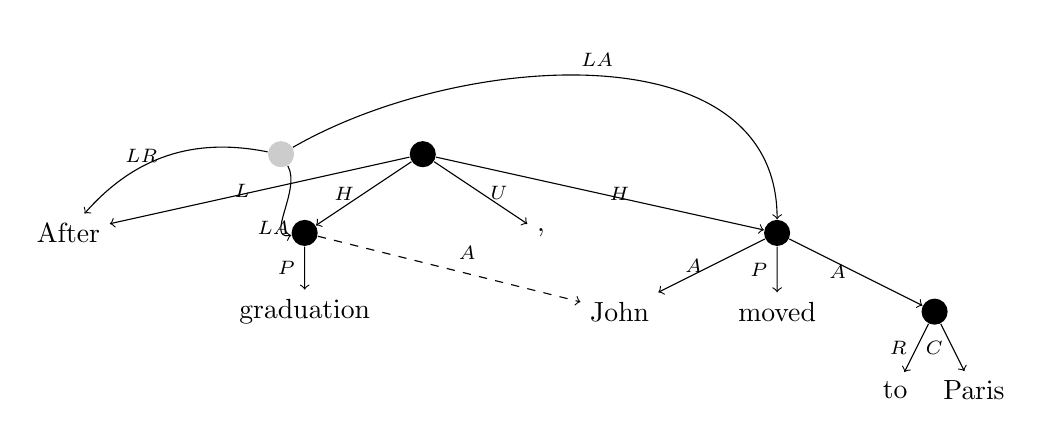
\begin{tikzpicture}[level distance=10mm, ->,
  level 1/.style={sibling distance=3cm},
  level 2/.style={sibling distance=2cm},
  level 3/.style={sibling distance=1cm}]
    \node (ROOT) [fill=black, circle] {}
      child {node (After) {After} edge from parent node[left] {\scriptsize $L$}}
      child {node (graduation) [fill=black, circle] {}
      {
        child {node {graduation} edge from parent node[left] {\scriptsize $P$}}
      } edge from parent node[left] {\scriptsize $H$} }
      child {node {,} edge from parent node[right] {\scriptsize $U$}}
      child {node (moved) [fill=black, circle] {}
      {
        child {node (John) {John} edge from parent node[left] {\scriptsize $A$}}
        child {node {moved} edge from parent node[left] {\scriptsize $P$}}
        child {node [fill=black, circle] {}
        {
          child {node {to} edge from parent node[left] {\scriptsize $R$}}
          child {node {Paris} edge from parent node[left] {\scriptsize $C$}}
        } edge from parent node[left] {\scriptsize $A$} }
      } edge from parent node[right] {\scriptsize $H$} }
      ;
    \draw[dashed,->] (graduation) to node [auto] {\scriptsize $A$} (John);
    \node (LKG) at (-1.8,0) [fill=black!20, circle] {};
          \draw[bend right] (LKG) to node [auto, left] {\scriptsize $LR$} (After);
          \draw (LKG) to[out=-60, in=190] node [below] {\scriptsize $LA\quad$} (graduation);
          \draw (LKG) to[out=30, in=90] node [above] {\scriptsize $LA$} (moved);
  \end{tikzpicture}
  \caption{UCCA example with linkage.}
  \label{fig:example_linkage}
\end{figure}

\paragraph{Implicit units.}

UCCA graphs may contain implicit units with no correspondent in the text.
\figref{fig:example_implicit} shows the annotation for the sentence
``A similar technique is almost impossible to apply to other crops, such as cotton, soybeans and rice.''.
The sentence was used by \newcite{oepen2015semeval} to compare between different semantic
dependency schemes.
It includes a single scene, whose main relation is ``apply'', a secondary relation ``almost impossible'', as well as two complex arguments: ``a similar technique'' and the coordinated argument ``such as cotton, soybeans, and rice.''
In addition, the scene includes an implicit argument, which represents the agent of the
``apply'' relation.

\begin{figure}[ht]
  \centering
  \scalebox{.5}{
  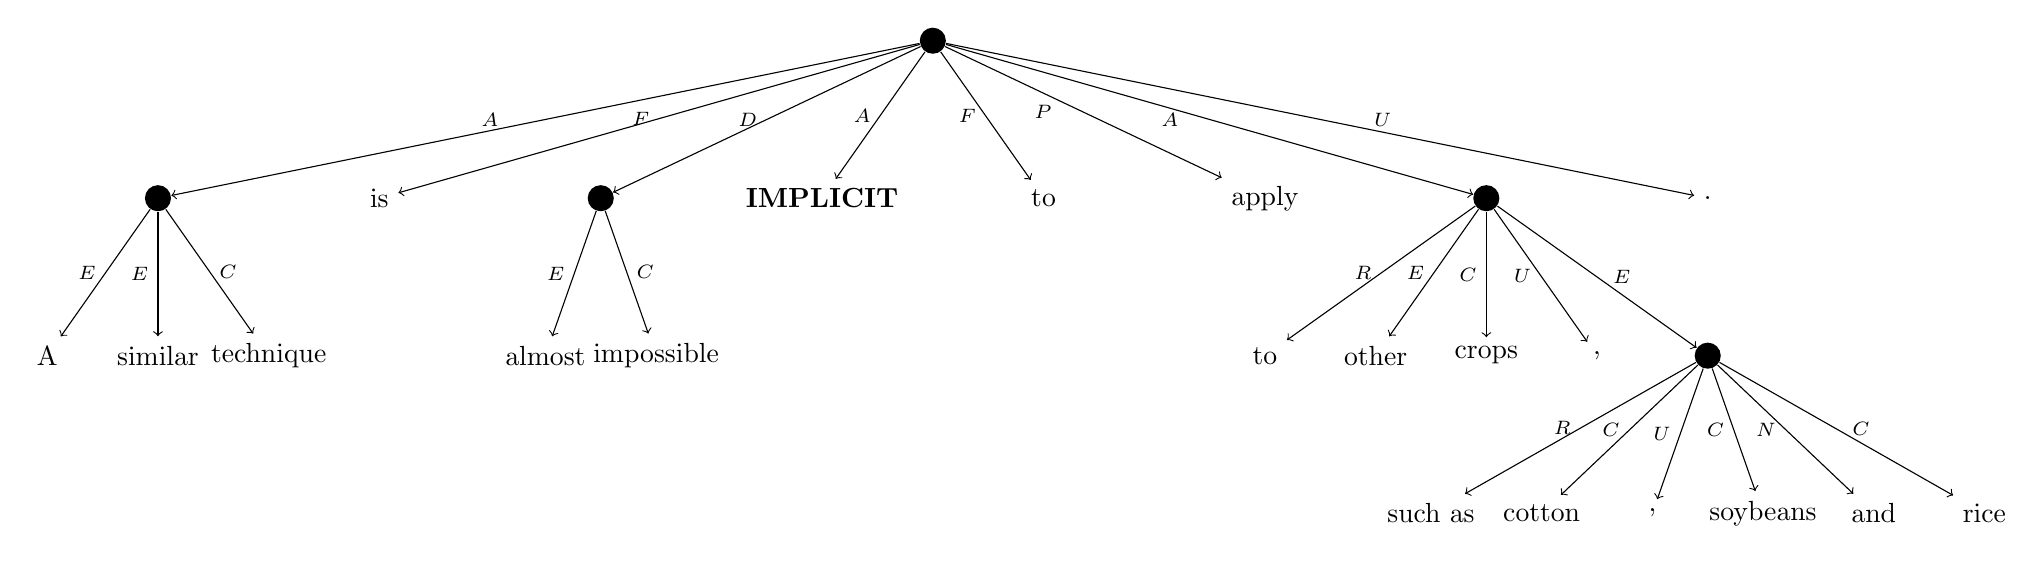
\begin{tikzpicture}[level distance=20mm, ->,
  level 1/.style={sibling distance=8em},
  level 2/.style={sibling distance=4em},
  level 3/.style={sibling distance=4em}]
    \node (ROOT) [fill=black, circle] {}
      child {node [fill=black, circle] {}
      {
        child {node {A} edge from parent node[left] {\scriptsize $E$}}
        child {node {similar} edge from parent node[left] {\scriptsize $E$}}
        child {node {technique} edge from parent node[right] {\scriptsize $C$}}
      } edge from parent node[left] {\scriptsize $A\quad$ \hspace{1mm} } }
      child {node {is} edge from parent node[left] {\scriptsize $F$}}
      child {node [fill=black, circle] {}
      {
        child {node {almost} edge from parent node[left] {\scriptsize $E$}}
        child {node {impossible} edge from parent node[right] {\scriptsize $C$}}
      } edge from parent node[left] {\scriptsize $D$} }
      child {node {\textbf{IMPLICIT}} edge from parent node[left] {\scriptsize $A$}}
      child {node {to} edge from parent node[left] {\scriptsize $F$}}
      child {node {apply} edge from parent node[left] {\scriptsize $P\quad$}}
      child {node [fill=black, circle] {}
      {
        child {node {to} edge from parent node[left] {\scriptsize $R$}}
        child {node {other} edge from parent node[left] {\scriptsize $E$}}
        child {node {crops} edge from parent node[left] {\scriptsize $C$}}
        child {node {,} edge from parent node[left] {\scriptsize $U$}}
        child {node [fill=black, circle] {}
        {
          child {node {such as} edge from parent node[left] {\scriptsize $R$}}
          child {node {cotton} edge from parent node[left] {\scriptsize $C$}}
          child {node {,} edge from parent node[left] {\scriptsize $U$}}
          child {node {soybeans} edge from parent node[left] {\scriptsize $C$}}
          child {node {and} edge from parent node[left] {\scriptsize $N$}}
          child {node {rice} edge from parent node[right] {\scriptsize $\; C$}}
        } edge from parent node[right] {\scriptsize $\; E$ \hspace{1mm} } }
      } edge from parent node[left] {\scriptsize $A\;$ \hspace{1mm} } }
      child {node {.} edge from parent node[right] {\scriptsize $\quad \quad U$}}
      ;
  \end{tikzpicture}
  }
  \caption{UCCA example with an implicit unit.}
  \label{fig:example_implicit}
\end{figure}

The parsing of these units is deferred to future work, as it is likely to require different methods
than those explored in this paper \cite{roth2015inducing}.

\section{Hyperparameter Values}
\label{appendix:hyperparameters}

\tabref{table:hyperparametersa} lists the hyperparameter values we found
for the different classifiers by tuning on the development set.
Note that learning rate decay is multiplicative and is applied at each epoch.
Mini-batch size is in number of transitions,
but a mini-batch must contain only whole sentences.

\begin{table}[ht]
\centering
\scalebox{.9}{
\begin{tabular}{l|ccc}
& Sparse & MLP & BiLSTM \\
\hline
\multicolumn{4}{l}{\footnotesize Embedding dimensions} \\
external word & & 100 & 100 \\
word & & 200 & 200 \\
POS tag & & 20 & 20 \\
syntactic dep. & & 10 & 10 \\
edge label & & 20 & 20 \\
punctuation & & 1 & 1 \\
gap & & 3 & 3 \\
action & & 3 & 3 \\\\\\\\\\
\end{tabular}
\begin{tabular}{||l|ccc}
& Sparse & MLP & BiLSTM \\
\hline
\multicolumn{4}{||l}{\footnotesize Other parameters} \\
training epochs & 19 & 28 & 59 \\
$\textsc{MinUpdate}$ & 5 \\
initial learning rate & 1 & 1 & 1 \\
learning rate decay & 0.1 & 1 & 1 \\
MLP \#layers & & 2 & 2 \\
MLP layer dim. & & 100 & 50 \\
LSTM \#layers & & & 2 \\
LSTM layer dim. & & & 500 \\
word dropout & & 0.2 & 0.2 \\
dropout & & 0.4 & 0.4 \\
weight decay & & $10^{-5}$ & $10^{-5}$ \\
mini-batch size & & 100 & 100
\end{tabular}
}
\caption{Hyperparameters used for the different classifiers.}
\label{table:hyperparametersa}
\end{table}

\section{Bilexical Graph Conversion}
\label{appendix:conversion}

Here we describe the algorithms used in the conversion referred to in \secref{sec:exp_setup}.

\paragraph{Notation.}
Let $L$ be the set of possible edge labels.
A UCCA graph over a sequence of tokens $w_1, \ldots, w_n$ is a directed acyclic graph
$G=(V,E, \ell)$, where $\ell:E\to L$ maps edges to labels.
For each token $w_i$ there exists a leaf (\emph{terminal}) $t_i \in V$.
A bilexical (dependency) graph over the same text consists of a set $A$ of
labeled dependency arcs $(t^\prime,l,t)$
between the terminals of $G$, where $t^\prime$ is the head, $t$ is the dependent and $l$ is
the edge label.

\paragraph{Conversion to bilexical graphs.}
Let $G=(V,E,\ell)$ be a UCCA graph with labels $\ell:E\rightarrow L$.
The conversion to a bilexical graph requires calculating the set $A$.
All non-terminals in $G$ are removed.

We define a linear order over possible edge labels $L$ (see \figref{fig:priority}).
The priority order generally places core-like categories before adjunct-like ones, and was decided heuristically.
For each node $u \in V$, denote by $h(u)$ its child with the highest-priority edge label.
The leftmost edge is chosen in case of a tie.
Let $h^*(u)$ be the terminal reached by recursively applying $h(\cdot)$ over $u$.
For each terminal $t$, we define
\[
N(t) = \{(u,v)\in E \;|\; t=h^*(v) \wedge t \neq h^*(u) \}
\]
For each edge $(u,v)\in N(t)$, we add $h^*(u)$ as a head of $t$ in $A$,
with the label $\ell(u,v)$.
This procedure is given in Algorithm~\ref{alg:to_bilexicala}.

\begin{figure}[H]
\begin{subfigure}{.52\textwidth}
\begin{algorithm}[H]
 \KwData{UCCA graph ${G}=(V,E,\ell)$}
 \KwResult{set $A$ of labeled bilexical arcs}
 $A \leftarrow \emptyset$\;
 \ForEach{$t \in \mathrm{Terminals}(V)$} {
  \ForEach{$(u,v)\in N(t)$} {
   $A \leftarrow A \cup \{(h^*(u), \ell(u, v), t)\}$\;
  }
 }
\end{algorithm}
 \caption{Conversion to bilexical graphs.}
 \label{alg:to_bilexicala}
\end{subfigure}\hfill
\begin{subfigure}{.49\textwidth}
\begin{multicols}{2}\scriptsize
\begin{enumerate}
\itemsep0em
\item $C$ (Center)
\item $N$ (Connector)
\item $H$ (ParallelScene)
\item $P$ (Process)
\item $S$ (State)
\item $A$ (Participant)
\item $D$ (Adverbial)
\item $T$ (Time)
\item $E$ (Elaborator)
\item $R$ (Relator)
\item $F$ (Function)
\item $L$ (Linker)
\item $LR$ (LinkRelation)
\item $LA$ (LinkArgument)
\item $G$ (Ground)
\item $\mathit{Terminal}$
\item $U$ (Punctuation)
\end{enumerate}
\end{multicols}
\caption{Priority order of edge labels used by $h(u)$.}
\label{fig:priority}
\end{subfigure}\caption{}
\end{figure}

Note that this conversion procedure
is simpler than the head percolation procedure used for converting syntactic constituency
trees to dependency trees \cite{Coll:97},
since $h(u)$ (similar to $u$'s head-containing child)
depends only on $\ell(u,h(u))$ and not on the sub-tree spanned by $u$,
because edge labels in UCCA directly express the role of the child in the parent unit, and
are thus sufficient for determining which of $u$'s children contains the head node.

\paragraph{Conversion from bilexical graphs.}
The inverse conversion introduces non-terminal nodes back into the graph.
As the distinction between low- and high-attaching nodes is lost in the
conversion, we assume that attachments are always
low-attaching.
Let $A$ be a the labeled arc set of a bilexical graph.
Iterating over the terminals in topological order according to $A$,
we add its members as terminals to graph
and create a pre-terminal parent $u_t$ for each terminal $t$,
with an edge labeled as \textit{Terminal} between them.
The parents of the pre-terminals are determined by the terminal's parent in the bilexical
graph: if $t^\prime$ is a head of $t$ in $A$, then $u_{t^\prime}$ will be a parent of $u_t$.
We add an intermediate node in between if $t$ has any dependents in $A$,
to allow adding their pre-terminals as children later.
Edge labels for the intermediate edges are determined by a rule-based function, denoted by
$\mathrm{Label}(t)$.
This procedure is given in Algorithm~\ref{alg:from_bilexical}.

\begin{algorithm}[ht]
 \KwData{list $T$ of terminals, set $A$ of labeled bilexical arcs}
 \KwResult{UCCA graph $G=(V,E,\ell)$}
 \SetKwFunction{Label}{Label}{}{}
 $V \leftarrow \emptyset$,
 $E \leftarrow \emptyset$\;
 \ForEach{$t \in \mathrm{TopologicalSort}(T, A)$} {
  $u_t \leftarrow \mathrm{Node()}$\;
  $V \leftarrow V \cup \{u_t, t\}$,
  $E \leftarrow E \cup \{(u_t, t)\}$\;
  $\ell(u_t,t)\leftarrow\mathit{Terminal}$\;
  \ForEach{$t^\prime\in T,l\in L$} {
   \If{$(t^\prime,l,t)\in A$} {
    \eIf{$\exists t^{\prime\prime}\in T,l^\prime\in L : (t,l^\prime,t^{\prime\prime}) \in A$} {
     $u \leftarrow \mathrm{Node()}$\;
     $V \leftarrow V \cup \{u\}$,
     $E \leftarrow E \cup \{(u, u_t)\}$\;
     $\ell(u, u_t) \leftarrow \Label(t)$\;
    } {
     $u \leftarrow u_t$\;
    }
    $E \leftarrow E \cup \{(u_{t^\prime}, u)\}$\;
    $\ell(u_{t^\prime}, u) \leftarrow l$\;
    }
  }
 }
 
  \SetKwProg{func}{Function}{}{}
  
  \func{\Label}{
  \KwData{node $t \in T$}
  \KwResult{label $l\in L$}

   \uIf{$\mathrm{IsPunctuation}(t)$}{
    \Return \textit{Punctuation}\;
   }
   \uElseIf{$\exists t^\prime \in T : (t,\textit{ParallelScene},t^\prime)\in A$}{
    \Return \textit{ParallelScene}\;
   }
   \uElseIf{$\exists t^\prime \in T : (t,\textit{Participant},t^\prime)\in A$}{
    \Return \textit{Process}\;
   }
   \uElse{
    \Return \textit{Center}\;
   }
  }
 \caption{Conversion from bilexical graphs.}
 \label{alg:from_bilexical}
\end{algorithm}

\section{Proof Sketch for Completeness of the \parser{} Transition Set}
\label{appendix:completeness_proof}

Here we sketch a proof for the fact that the transition set defined in \secref{sec:parser}
is capable of producing any rooted, labeled, anchored DAG.
This proves that the transition set is complete with respect to the class of graphs that
comprise UCCA.

Let $G=(V,E,\ell)$ be a graph with labels $\ell:E\rightarrow L$
over a sequence of tokens $w_1, \ldots, w_n$.
Parsing starts with $w_1, \ldots, w_n$ on the buffer,
and the root node on the stack.

First we show that every node can be created, by induction on the node height:
every terminal (height zero) already exists at the beginning of the parse
(and so does the root node).
Let $v\in V$ be of height $k$, and assume all nodes of height less than $k$ can be created.
Take any (primary) child $u$ of $v$: its height must be less than $k$.
If $u$ is a terminal, apply \textsc{Shift} until it lies at the head of the buffer.
Otherwise, by our assumption, $u$ can still be created.
Right after $u$ is created, it lies at the head of the buffer.
A \textsc{Shift} transition followed by a \textsc{Node}$_{\ell(v,u)}$ transition will
move $u$ to the stack and create $v$ on the buffer, with the correct edge label.

Next, we show that every edge can be created.
Let $(v,u) \in E$ be any edge with parent $v$ and child $u$.
Assume $v$ and $u$ have both been created (we already showed that both are created eventually).
If either $v$ or $u$ are in the buffer, apply \textsc{Shift} until both are in the stack.
If both are in the stack but neither is at the stack top, apply \textsc{Swap} transitions
until either moves to the buffer, and then apply \textsc{Shift}.
Now, assume either $v$ or $u$ is at the stack top.
If the other is not the second element on the stack, apply \textsc{Swap} transitions until it is.
Finally, $v$ and $u$ are the top two elements on the stack.
If they are in that order, apply \textsc{Right-Edge}$_{\ell(v,u)}$
(or \textsc{Right-Remote}$_{\ell(v,u)}$ if the edge between them is remote).
Otherwise, apply \textsc{Left-Edge}$_{\ell(v,u)}$
(or \textsc{Left-Remote}$_{\ell(v,u)}$ if the edge between them is remote).
This creates $(v,u)$ with the correct edge label.

Once all nodes and edges have been created, we can apply \textsc{Reduce} until only the
root node remains on the stack, and then \textsc{Finish}.
This yields exactly the graph $G$.

Note that the distinction we made between primary and remote transitions is suitable for UCCA parsing.
For general graph parsing without this distinction,
the \textsc{Remote} transitions can be removed, as well as the single-primary-parent
restriction on \textsc{Edge} transition.

%
% File acl2018_supp.tex
%
\chapter{Multitask Parsing Across Semantic Representations \\ Supplementary Notes}

\section{Features}

Table~\ref{tab:features} lists all feature used for the classifier (see \S\ref{sec:classifier}).
Numeric features are taken as they are, whereas categorical features are mapped to real-valued embedding
vectors.
For \texttt{w} features,
we concatenate randomly-initialized and pre-trained word embeddings.
For each node, we select a \textit{head terminal} by traversing the graph according to
a priority order on edge labels, taken from \citet{hershcovich2017a}.

$s_i$ refers to stack node $i$ from the top, and
$b_i$ to buffer node $i$.
$xl$ and $xr$ refer to a $x$'s leftmost and rightmost children, and
$xL$ and $xR$ to its leftmost and rightmost parents.

\texttt{w} refers to the node's head terminal text,
\texttt{t} to its POS tag, and
\texttt{d} to its dependency relation.
\texttt{h} refers to the node's height,
\texttt{e} to the tag of its first incoming edge,
\texttt{n} and \texttt{c} to the node label and category (used only for AMR),
\texttt{p} to any separator punctuation between $s_0$ and $s_1$,
\texttt{q} to the count of any separator punctuation between $s_0$ and $s_1$,
\texttt{x} to the numeric value of gap type \cite{maier-lichte:2016:DiscoNLP},
\texttt{y} to the sum of gap lengths,
\texttt{P}, \texttt{C}, \texttt{I}, \texttt{E}, and \texttt{M} to the number of
parents, children, implicit children, remote children, and remote parents,
\texttt{N} to the numeric value of the head terminal's named entity IOB indicator,
\texttt{T} to its named entity type,
\texttt{\#} to its word shape (capturing orthographic features, e.g. "Xxxx" or "dd"),
\texttt{\^{}} to its one-character prefix, and
\texttt{\$} to its three-character suffix.

$x \to y$ refers to the existing edge from $x$ to $y$.
\texttt{x} is an indicator feature, taking the value of 1 if the edge exists or 0 otherwise,
\texttt{e} refers to the edge label, and
\texttt{d} to the dependency distance between the head terminals of the nodes.

$a_i$ to the transition taken $i+1$ steps ago.
\texttt{A} refers to the action type label (e.g. \textsc{shift}/\textsc{right-edge}/\textsc{node}), and
\texttt{e} to the edge label created by the action (e.g. $C$/$E$/$P$).

\texttt{node ratio} is the ratio between non-terminals and terminals, taken from \citet{hershcovich2017a}.

\begin{table}[h]
\centering
\begin{tabular}{l|l}
\bf Nodes & \bf Features \\ 
\hline
%       w   t   d   e   n   c   p   T   #   ^   $   x   h   q   y   P   C   I   E   M   N
$s_0$ & \texttt{wtdencpT\#\^{}\$xhqyPCIEMN} \\
$s_1$ & \texttt{wtdencT\#\^{}\$xhyN} \\
$s_2$ & \texttt{wtdencT\#\^{}\$xhy} \\
$s_3$ & \texttt{wtdencT\#\^{}\$xhyN} \\
$b_0$ & \texttt{wtdncT\#\^{}\$hPCIEMN} \\
$b_1, b_2, b_3$ & \texttt{wtdncT\#\^{}\$} \\
$s_0l, s_0r, s_1l, s_1r, s_0ll, s_0lr, s_0rl, s_0rr, s_1ll, s_1lr, s_1rl, s_1rr$ &
    \texttt{wenc\#\^{}\$} \\
$s_0L, s_0R, s_1L, s_1R, b_0L, b_0R$ & \texttt{wen\#\^{}\$} \\
\hline
\bf Edges & \\
$s_0 \to s_1, s_0 \to b_0$ & \texttt{xd} \\
$s_1 \to s_0, b_0 \to s_0$ & \texttt{x} \\
$s_0 \to b_0, b_0 \to s_0$ & \texttt{e} \\
\hline
\bf Past actions \\
$a_0, a_1$ & \texttt{eA} \\
\hline
\bf Misc. & \texttt{node ratio}
\end{tabular}
\caption{Transition classifier features.\label{tab:features}}
\end{table}


\section{Conversion to and from Unified DAG Format}

Although all experiments reported in the paper with the auxiliary tasks
(AMR, DM and UD) are using unlabeled parsing for these schemes,
our conversion code supports full conversion to and from these formats,
and is publicly available at \url{http://github.com/danielhers/semstr/tree/master/semstr/conversion}.

Conversion from AMR to the unifid DAG format and back
results in 95\% Smatch $F_1$ \cite{cai2013smatch} when averaged over the
LDC2017T10 test set.
On SDP, the conversion is lossless and results in identical graphs
when converted to UCCA and back.
For UD, and conversion results in 98.5\% LAS $F_1$ on the UD English test set,
due to multi-word tokens, not supported in the unified DAG format.

\section{Qualitative evaluation}

Figure~\ref{fig:qualitative} shows an example sentence from the English 20K test set,
with the outputs of both our single-task model and our best MTL model (using all auxiliaries).
While the single-task model obtains an $F_1$ score of 67.9\% on this sentence, the MTL model's output
matches the gold-annotates graph perfectly.
This example demonstrates how
the parser's ability to identify syntactic constituents,
which is important for all tasks we tackled, is improved with MTL.


\begin{sidewaysfigure}
    \centering
\scalebox{.6}{
\begin{tikzpicture}[->,level distance=26mm,
  level 1/.style={sibling distance=16cm},
  level 2/.style={sibling distance=7cm},
  level 3/.style={sibling distance=2cm},
  every circle node/.append style={fill=black}]
  \tikzstyle{word} = [font=\rmfamily,color=black]
  \node (1_1) [circle] {}
  {
  child {node (1_2) [circle] {}
    {
    child {node (1_5) [circle] {}
      {
      child {node (1_10) [word] {No} edge from parent node[auto] {\scriptsize $E$}}
      child {node (1_11) [word] {transoceanic} edge from parent node[auto] {\scriptsize $E$}}
      child {node (1_12) [word] {navigational} edge from parent node[auto] {\scriptsize $E$}}
      child {node (1_13) [word] {undertaking} edge from parent node[auto] {\scriptsize $C$}} }edge from parent node[auto] {\scriptsize $A$}}
    child {node (1_6) [circle] {}
      {
      child {node (1_14) [word] {has} edge from parent node[auto] {\scriptsize $F$}}
      child {node (1_15) [word] {been} edge from parent node[auto] {\scriptsize $E$}}
      child {node (1_16) [word] {conducted} edge from parent node[auto] {\scriptsize $C$}} }edge from parent node[auto] {\scriptsize $P$}}
    child {node (1_7) [circle] {}
      {
      child {node (1_17) [word] {with} edge from parent node[auto] {\scriptsize $R$}}
      child {node (1_18) [circle] {}
        {
        child {node (1_25) [circle] {}
          {
          child {node (1_28) [word] {more} edge from parent node[auto] {\scriptsize $E$}}
          child {node (1_29) [word] {ability} edge from parent node[auto] {\scriptsize $C$}} }edge from parent node[auto] {\scriptsize $C$}}
        child {node (1_26) [word] {,} edge from parent node[auto] {\scriptsize $U$}}
        child {node (1_27) [circle] {}
          {
          child {node (1_30) [word] {no} edge from parent node[auto] {\scriptsize $E$}}
          child {node (1_31) [circle] {}
            {
            child {node (1_32) [word] {business} edge from parent node[auto] {\scriptsize $E$}}
            child {node (1_33) [word] {dealings} edge from parent node[auto] {\scriptsize $C$}} }edge from parent node[auto] {\scriptsize $C$}} }edge from parent node[auto] {\scriptsize $C$}} }edge from parent node[auto] {\scriptsize $C$}} }edge from parent node[auto] {\scriptsize $A$}} }edge from parent node[auto] {\scriptsize $H$}}
  child {node (1_3) [circle] {}
    {
    child {node (1_8) [circle] {}
      {
      child {node (1_19) [word] {have} edge from parent node[auto] {\scriptsize $F$}}
      child {node (1_20) [word] {been} edge from parent node[auto] {\scriptsize $E$}}
      child {node (1_21) [word] {crowned} edge from parent node[auto] {\scriptsize $C$}} }edge from parent node[auto] {\scriptsize $P$}}
    child {node (1_9) [circle] {}
      {
      child {node (1_22) [word] {with} edge from parent node[auto] {\scriptsize $R$}}
      child {node (1_23) [word] {greater} edge from parent node[auto] {\scriptsize $D$}}
      child {node (1_24) [word] {success} edge from parent node[auto] {\scriptsize $P$}} }edge from parent node[auto] {\scriptsize $A$}} }edge from parent node[auto] {\scriptsize $H$}}
  child {node (1_4) [word] {.} edge from parent node[auto] {\scriptsize $U$}} }
;
\end{tikzpicture}}
\scalebox{.6}{
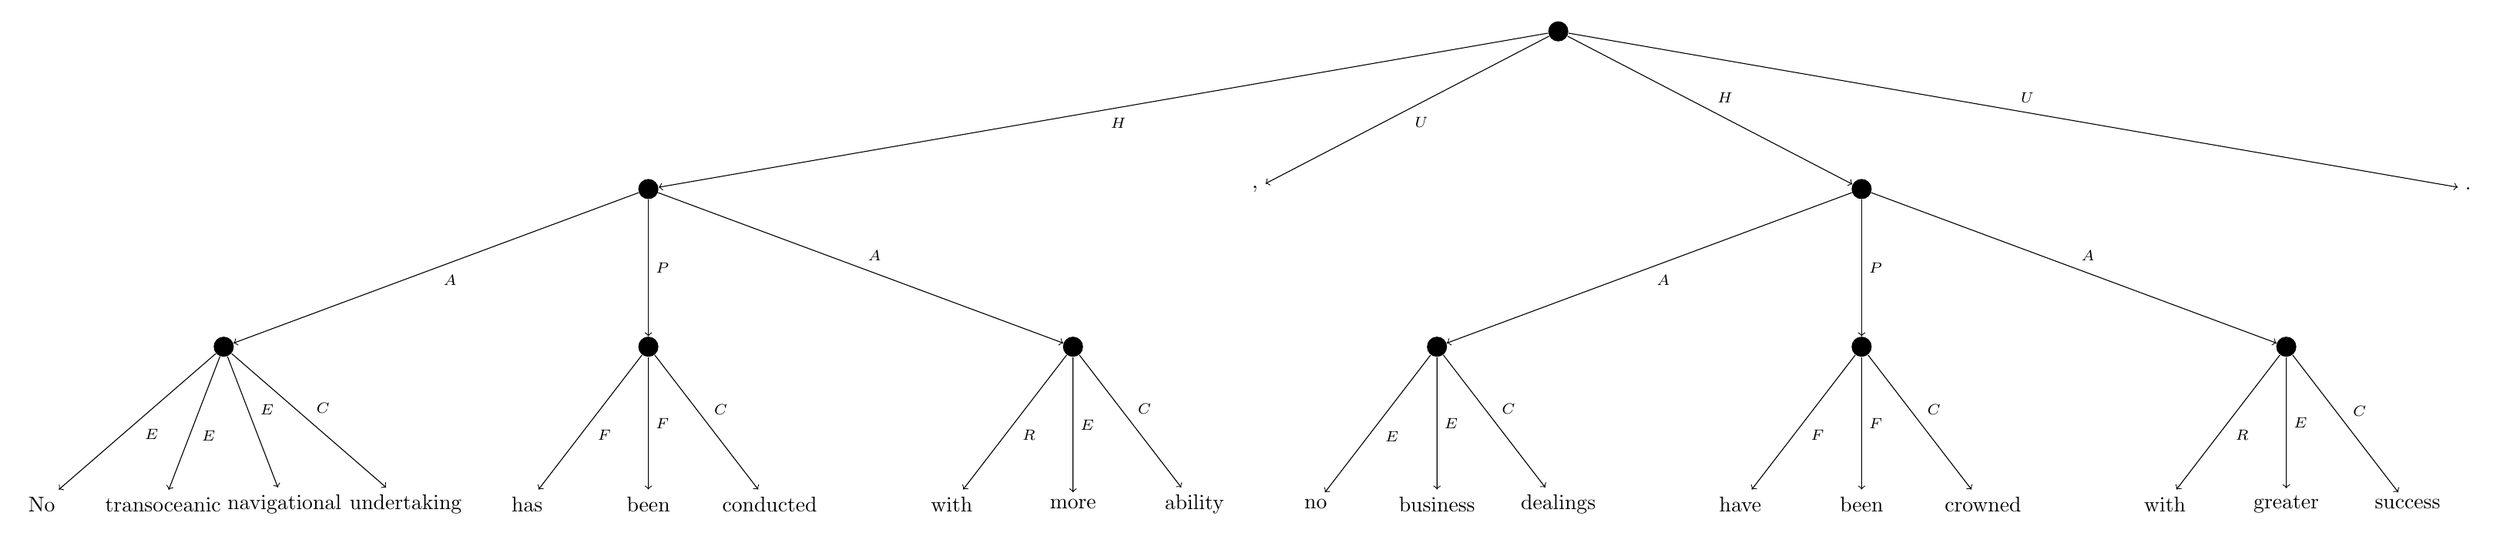
\begin{tikzpicture}[->,level distance=26mm,
      level 1/.style={sibling distance=10cm},
      level 2/.style={sibling distance=7cm},
      level 3/.style={sibling distance=2cm},
  every circle node/.append style={fill=black}]
  \tikzstyle{word} = [font=\rmfamily,color=black]
  \node (1_1) [circle] {}
  {
  child {node (1_2) [circle] {}
    {
    child {node (1_6) [circle] {}
      {
      child {node (1_12) [word] {No} edge from parent node[auto] {\scriptsize $E$}}
      child {node (1_13) [word] {transoceanic} edge from parent node[auto] {\scriptsize $E$}}
      child {node (1_14) [word] {navigational} edge from parent node[auto] {\scriptsize $E$}}
      child {node (1_15) [word] {undertaking} edge from parent node[auto] {\scriptsize $C$}} }edge from parent node[auto] {\scriptsize $A$}}
    child {node (1_7) [circle] {}
      {
      child {node (1_16) [word] {has} edge from parent node[auto] {\scriptsize $F$}}
      child {node (1_17) [word] {been} edge from parent node[auto] {\scriptsize $F$}}
      child {node (1_18) [word] {conducted} edge from parent node[auto] {\scriptsize $C$}} }edge from parent node[auto] {\scriptsize $P$}}
    child {node (1_8) [circle] {}
      {
      child {node (1_19) [word] {with} edge from parent node[auto] {\scriptsize $R$}}
      child {node (1_20) [word] {more} edge from parent node[auto] {\scriptsize $E$}}
      child {node (1_21) [word] {ability} edge from parent node[auto] {\scriptsize $C$}} }edge from parent node[auto] {\scriptsize $A$}} }edge from parent node[auto] {\scriptsize $H$}}
  child {node (1_3) [word] {,} edge from parent node[auto] {\scriptsize $U$}}
  child {node (1_4) [circle] {}
    {
    child {node (1_9) [circle] {}
      {
      child {node (1_22) [word] {no} edge from parent node[auto] {\scriptsize $E$}}
      child {node (1_23) [word] {business} edge from parent node[auto] {\scriptsize $E$}}
      child {node (1_24) [word] {dealings} edge from parent node[auto] {\scriptsize $C$}} }edge from parent node[auto] {\scriptsize $A$}}
    child {node (1_10) [circle] {}
      {
      child {node (1_25) [word] {have} edge from parent node[auto] {\scriptsize $F$}}
      child {node (1_26) [word] {been} edge from parent node[auto] {\scriptsize $F$}}
      child {node (1_27) [word] {crowned} edge from parent node[auto] {\scriptsize $C$}} }edge from parent node[auto] {\scriptsize $P$}}
    child {node (1_11) [circle] {}
      {
      child {node (1_28) [word] {with} edge from parent node[auto] {\scriptsize $R$}}
      child {node (1_29) [word] {greater} edge from parent node[auto] {\scriptsize $E$}}
      child {node (1_30) [word] {success} edge from parent node[auto] {\scriptsize $C$}} }edge from parent node[auto] {\scriptsize $A$}} }edge from parent node[auto] {\scriptsize $H$}}
  child {node (1_5) [word] {.} edge from parent node[auto] {\scriptsize $U$}} }
;
\end{tikzpicture}}
\caption{Output of single-task model on sentence 53001 from the English 20K test set (top),
and of MTL model using all of AMR, DM and UD$^{++}$ as auxiliaries on the same sentence (bottom).
\label{fig:qualitative}}
\end{sidewaysfigure}


%
% File divergences_supp.tex

\chapter{Content Differences in Syntactic and Semantic Representation \\ Supplementary Material}

\section{UCCA Category Definitions}\label{sec:definitions}

Table~\ref{tab:ucca} provides a concise description of the
categories used by the UCCA foundational layer.

\begin{table}[H]
\centering
\footnotesize
\begin{tabular}{cp{2cm}p{12.5cm}}
\multicolumn{3}{c}{\bf Scene Elements}\\
P & {\bf Process} & The main relation of a Scene that evolves in time (usually an action or movement).\\
S & {\bf State} & The main relation of a Scene that does not evolve in time.\\
A & {\bf Participant} & A participant in a Scene in a broad sense (including locations, abstract entities and Scenes serving as arguments).\\
D & {\bf Adverbial} & A secondary relation in a Scene.\\
T & {\bf Time} & A temporal relation in a Scene.\\
\multicolumn{3}{c}{{\bf Elements of Non-Scene Units}}\\
C & {\bf Center} & Necessary for the conceptualization of the parent unit.\\
E & {\bf Elaborator} & A non-Scene relation which applies to a single Center.\\
N & {\bf Connector} & A non-Scene relation which applies to two or more Centers, highlighting a common feature.\\
R & {\bf Relator} & All other types of non-Scene relations. Two varieties: (1) Rs that relate a C to some super-ordinate relation, and
(2) Rs that relate two Cs pertaining to different aspects of the parent unit. \\
Q & {\bf Quantifier} & Describing the quantity or magnitude of something, or defines an entity as a group or a set (e.g., ``two'' or ``a group of'').\\
\multicolumn{3}{c}{\bf Inter-Scene Relations}\\
H & {\bf Parallel Scene} & A Scene linked to other Scenes by regular linkage (e.g., temporal, logical, purposive).\\
L & {\bf Linker} & A relation between two or more Hs (e.g., ``when'', ``if'', ``in order to'').\\
G & {\bf Ground} & A relation between the speech event and the uttered Scene (e.g., ``surprisingly'', ``in my opinion'').\\
\multicolumn{3}{c}{\bf Other}\\
F & {\bf Function} & Does not introduce a relation or participant. Required by the structural pattern it appears in.
\end{tabular}
\caption{The complete set of categories in UCCA's foundational layer.\label{tab:ucca}}
\end{table}

\section{Universal Dependencies Category Definitions}

Table~\ref{tab:ud} lists the full names of the
relation labels used by Universal Dependencies v2.

\begin{table}[H]
\footnotesize
\begin{multicols}{2}
\texttt{acl} clausal modifier of noun (adjectival clause) \\
\texttt{advcl} adverbial clause modifier \\
\texttt{advmod} adverbial modifier \\
\texttt{amod} adjectival modifier \\
\texttt{appos} appositional modifier \\
\texttt{aux} auxiliary \\
\texttt{case} case marking \\
\texttt{cc} coordinating conjunction \\
\texttt{ccomp} clausal complement \\
\texttt{clf} classifier \\
\texttt{compound} compound \\
\texttt{conj} conjunct \\
\texttt{cop} copula \\
\texttt{csubj} clausal subject \\
\texttt{dep} unspecified dependency \\
\texttt{det} determiner \\
\texttt{discourse} discourse element \\
\texttt{dislocated} dislocated elements \\
\texttt{expl} expletive \\
\texttt{fixed} fixed multiword expression \\
\texttt{flat} flat multiword expression \\
\texttt{goeswith} goes with \\
\texttt{iobj} indirect object \\
\texttt{list} list \\
\texttt{mark} marker \\
\texttt{nmod} nominal modifier \\
\texttt{nsubj} nominal subject \\
\texttt{nummod} numeric modifier \\
\texttt{obj} object \\
\texttt{obl} oblique nominal \\
\texttt{orphan} orphan \\
\texttt{parataxis} parataxis \\
\texttt{punct} punctuation \\
\texttt{reparandum} overridden disfluency \\
\texttt{root} root \\
\texttt{vocative} vocative \\
\texttt{xcomp} open clausal complement
\end{multicols}
\caption{UD v2 relations.\label{tab:ud}}
\end{table}



\pagebreak

\section*{\flushright{\heb{תקציר}}}

\begin{flushright}
\heb{מאמץ רב בעיבוד שפה טבעית מוקדש להבנת שפה טבעית, תחום אשר שם לעצמו כמטרה להיות מסוגל להבין טקסט,
להקיש ממנו היסקים, ולפעול על פיו באופן מלומד. בעוד לשימושים מסויימים ניתן להשתמש בשיטות פשוטות יחסית,
אשר מתעלמות לחלוטין מסדר המלים )מודלים מסוג שק מלים( או מתייחסות אליו כשרשרת פשוטה
)כמו שיטת הרצף-לרצף הנפוצה, המאפשרת לרשתות נוירונים ללמוד משימות באופן כולל(, הבנת טקסט באופן כללי דורשת
ייצוג היררכי של משמעות. בניית ייצוג זה מהטקסט היא מטרתה של סדרת עבודות רחבה בתחום הניתוח הסמנטי.
בעוד ייצוגים סמנטיים רבים הוצעו עד כה, יש ביניהם הרבה מן המשותף בנוגע לאבחנות הבסיסיות, כמו למשל בין
פרדיקטים )יחסים, מצבים ואירועים( ובין ארגומנטים )משתתפים(.}

\heb{תזה זו מתמקדת בייצוג סמנטי מסויים בשם ACCU, אשר העקרונות המנחים העיקריים שלו הם
תמיכה בכל התופעות הלשוניות הסמנטיות, תמיכה ויציבות בין שפות, קלות התיוג )אפילו בידי מי שאינו מומחה בבלשנות(,
וארכיטקטורה מודולרית התומכת בשכבות שונות של אנוטציה סמנטית.
מנתח אוטומטי לחלוטין מוצע במסגרת התזה, ומוערך על פני מספר שפות )אנגלית, צרפתית וגרמנית(.
המנתח, אשר שמו APUT, מסוגל ללמוד מבנים גרפיים כללים ביותר: גרפים מכוונים חסרי מעגלים על-פני
סדרות של מלים עם צמתים פנימיים עבור יחידות מורכבות, אשר יכולים לכסות סדרות לא רצופות של מלים.
המחלקה הכללית הזו של גרפים מכסה את המבנים אשר מתוייגים ב-ACCU, וגם ייצוגים אחרים.
APUT ממומש כמנתח מבוסס מעברים, אשר מערכת המעברים שלו תומכת בתכונות המבניות הללו.
מסווג המעברים של APUT הוא רשת נוירונים בעלת רכיב MTSLiB לחישוב ייצוגים עבור הקלט.
בהשוואה נרחבת לעומת שיטות המבוססות על המרה למבנים פשוטים יותר, וגם בהשוואה למימושים אחרים של המסווג,
נמצא ש-APUT מסוגל לנתח בדיוק רב יותר טקסט למבני ACCU, גם במצב שבו אוסף הבדיקה דומה לאוסף האימון
וגם כאשר הוא נלקח ממקור שונה. תוצאות אלו מודגמות בשלוש שפות.}

\heb{יכולתו של המנתח מודגמת גם לשתי שיטות אחרות לניתוח סמנטי, MD ו-RMA,
וגם לניתוח תחבירי בשיטת DU. ניסוי זה מדגים את גמישותו של המנתח, ואת יכולתו להתמודד
עם משימות נוספות מלבד ACCU. בנוסף, כאשר מאמנים את APUT על מספר משימות בעת ובעונה אחת,
ביצועיו משתפרים על ACCU. שיפור זה נעשה באמצעות למידה של הכללות הנוגעות לכל המשימות וחשובות להן.}

\heb{לבסוף, בהשוואה אמפירית של התוכן בייצוגים סמנטיים ותחביריים, אנו מגלים פנים שונים של הבדל ביניהם.
להבדלים אלו יש משמעות רבה בנוגע לתרומה של תחביר לניתוח סמנטי, ועל השימושיות של כל אחת מהשיטות למשימות
סמנטיות בעיבוד שפה טבעית.}

\heb{אני רואה בניתוח סמנטי אמצעי עבור מחשבים ללמוד שפה אנושית.
בעוד ייצוגים שונים מתמקדים באבחנות שונות באמצעות מבנים פורמליים שונים,
הם חולקים מטרה משותפת, לתמוך ביישומים של עיבוד שפה טבעית, כמו למשל
סיווג טקסט לקטגוריות, תיוג לפי תכונות בלשניות,
הסקת מסקנות,
וייצור טקסט חדש לפי אילוצים מסויימים )כמו בתרגום מכונה(.
מאגרי המידע המתויגים בכל הייצוגים הם משאב יקר-ערך,
אשר ניתן להשתמש בו להשגת שיפור ניכר בעיבוד והבנה של שפה טבעית.}
\end{flushright}

\pagebreak

\clearpage

\title{}
\author{
\heb{עבודה זו נעשתה בהדרכתם של} \\
\heb{פרופ' ארי רפופורט וד"ר עמרי אבנד}}
\date{}

\maketitle
\clearpage

\title{
\textbf{\heb{ניתוח סמנטי אוניברסלי באמצעות רשתות נוירונים}} \\
\vspace{2cm}
{\large\heb{חיבור לשם קבלת תואר דוקטור לפילוסופיה}}
}
\author{
\heb{מאת}\\
\heb{דניאל הרשקוביץ}
\vspace{2cm}
}
\date{
\heb{הוגש לסנט האוניברסיטה העברית בירושלים} \\
\heb{פברואר 9102}
}

\maketitle
\maketitle

\end{document}
